\PassOptionsToPackage{naturalnames}{hyperref}
\PassOptionsToPackage{dvipsnames,table,xcdraw}{xcolor}
\documentclass[8pt]{beamer}
\geometry{paperwidth=160mm,paperheight=90mm}
% loaded by beamer
% \usepackage[dvipsnames,table,xcdraw]{xcolor}
\usetheme[numbering=fraction]{metropolis}
\usecolortheme{beaver}
\setbeamercolor{background canvas}{bg=white}
% If you have more than one page of references, you want to tell beamer
% to put the continuation section label from the second slide onwards
\setbeamertemplate{frametitle continuation}[from second]
\setbeamertemplate{footline}{\begin{beamercolorbox}[wd=\textwidth,sep=3ex]{footline}\usebeamerfont{page number in head/foot}%
    \usebeamertemplate*{frame footer}
    \hfill%
    \textcolor{gray}{\insertsection}\space    
    \usebeamertemplate*{frame numbering}
  \end{beamercolorbox}%
}

% text encoding
\usepackage[utf8]{inputenc}
\usepackage[english]{babel}
\usepackage[T1]{fontenc}
\usepackage{lmodern}


% Greek letters in text
\usepackage{textgreek}

% quotations
\usepackage{fvextra} % to avoid warning in the next package
\usepackage{csquotes}


\usepackage{amsmath}
\usepackage{amsfonts}
\usepackage{amssymb}
\usepackage{physics}
\usepackage{siunitx}
\usepackage{gensymb}

\sisetup{per-mode=fraction}
% molar unit is added
\DeclareSIUnit\molar{M}

\DeclareMathOperator{\cov}{\text{cov}}
\DeclareMathOperator{\E}{\text{E}}
\DeclareMathOperator{\sign}{sgn}

% transpose version of T
\newcommand{\trans}{\intercal}

% environment to write descriptions of variables
\newenvironment{conditions}
  {\par\vspace{\abovedisplayskip}\noindent\begin{tabular}{>{$}l<{$} @{${}={}$} l}}
  {\end{tabular}\par\vspace{\belowdisplayskip}}


\usepackage{float} % better positioning of images
\usepackage{graphicx}
\usepackage[font={small,it}]{caption}
\usepackage{subcaption}
% to wrap text around figure so it can be displayed next to text
\usepackage{wrapfig}
\usepackage{sidecap}


% add figure list
\graphicspath{{./fig/}}
\usepackage{listings}


\usepackage{tabularx}
% define Y column type that is X with centering
\newcolumntype{Y}{>{\centering\arraybackslash}X}
% creates a type R to specify right adjustment instead of left
\newcolumntype{R}{>{\raggedleft\arraybackslash}X}
\usepackage{wrapfig}
\usepackage{booktabs}
% make it possible to make tables span more than one page
\usepackage{ltxtable}
% add boxes functionality to force line break in table cell
\usepackage{pbox}

% make a good looking tilde
\newcommand{\realtilde}{\raisebox{0.5ex}{\texttildelow}}


% appendix
% \usepackage[toc,page]{appendix}
% appendix is not defined implicitly
% \newcommand*{\Appendixautorefname}{Appendix}


% makes sure figures and tables stay in their section
\usepackage[section]{placeins}

% justification is raggedright (i.e. left aligned)
% singlelinecheck=off means that the justification setting is used even when the caption is only a single line long. 
% if singlelinecheck=on, then caption is always centered when the caption is only one line.
\captionsetup[subfigure]{singlelinecheck=off,justification=raggedright}

% % if you want to add numbering on parapraphs
% \usepackage{titlesec}
% % \setcounter{secnumdepth}{4}
% \titleformat{\paragraph}
% {\normalfont\normalsize\bfseries}{\theparagraph}{1em}{}
% \titlespacing*{\paragraph}
% {0pt}{3.25ex plus 1ex minus .2ex}{1.5ex plus .2ex}

\usepackage{array} % don't know what is used for

% nomenclature
% \usepackage{nomencl}

% bibliography. Maybe use bibtex instead of biber as backend
\usepackage[backend=biber,sorting=none,style=numeric]{biblatex}
\AtEveryBibitem{%
  \clearfield{issn} % Remove issn
  \clearfield{isbn} % Remove issn
  \clearfield{doi} % Remove doi

  \ifentrytype{misc}{}{% Remove url except for @misc
    \clearfield{url}
  }
}
\addbibresource{references.bib}
% import after adding bibliography in main in order to unescape _ and ~ in urls
\DeclareSourcemap{
\maps{
% Replaces '{\_}', '{_}' or '\_' with just '_'
    \map{
        \step[fieldsource=url,
            match=\regexp{\{\\\_\}|\{\_\}|\\\_},replace=\regexp{\_}]
        }
    \map{
        \step[fieldsource=doi,
            match=\regexp{\{\\\_\}|\{\_\}|\\\_},replace=\regexp{\_}]
        }
% Replaces '{'$\sim$'}', '$\sim$' or '{~}' with just '~'
    \map{ 
        \step[fieldsource=url,
            match=\regexp{\{\$\\sim\$\}|\{\~\}|\$\\sim\$},replace=\regexp{\~}]
        }
    \map{ 
        \step[fieldsource=doi,
            match=\regexp{\{\$\\sim\$\}|\{\~\}|\$\\sim\$},replace=\regexp{\~}]
        }
    }
}

% make bibliography entries smaller
\renewcommand\bibfont{\tiny}
% replace weird icon with numbering
\setbeamertemplate{bibliography item}{\insertbiblabel}


% header
\usepackage{fancyhdr}
\setlength{\headheight}{15.2pt}
% paragraphs of text start with no indent
\setlength{\parindent}{0pt}
% paragraphs of text start with a little skip from last text
\setlength{\parskip}{1ex plus 0.5ex minus 0.2ex}

% this package gives us minted to show code and Verbatim to set verbatim font size
\usepackage{minted}
\usepackage{parskip}
\definecolor{LightGray}{gray}{0.97}
\setminted[python]{baselinestretch=1.2,tabsize=4,bgcolor=LightGray,fontsize=\footnotesize,linenos}
\setminted[bash]{baselinestretch=1.2,bgcolor=LightGray,fontsize=\footnotesize,linenos}


% hyperref uses xcolor 
\usepackage{hyperref}
\hypersetup{
  linkcolor  = violet,
  citecolor  = YellowOrange,
  urlcolor   = Aquamarine,
  colorlinks = true,
}
% alt to hyperref's autoref
\usepackage{cleveref}

% insert image in title page or other difficult place
\usepackage{tikz}
\usetikzlibrary{positioning}




\definecolor{tf}{RGB}{119, 135, 68}
\definecolor{gene}{RGB}{155, 143, 76}
\definecolor{pk}{RGB}{102, 80, 127}

\makeatletter
\def\pk_#1{\textcolor{pk}{
\text{PK}_{#1}\@ifnextchar[{\pkbrac}{\relax}}}
\def\pkbrac[#1]{#1}
\def\tf_#1{\textcolor{tf}{
\text{TF}_{#1}\@ifnextchar[{\tfbrac}{\relax}}}
\def\tfbrac[#1]{#1}
\def\gene_#1{\textcolor{gene}{
\text{gene}_{#1}\@ifnextchar[{\genebrac}{\relax}}}
\def\genebrac[#1]{#1}
\makeatother


\begin{document}

% center titles

\setbeamertemplate{title}{
  \centering
  \linespread{1.0}%
  \inserttitle%
  \par%
  \vspace*{0.5em}
}
\setbeamertemplate{subtitle}{
  \centering
  \insertsubtitle%
  \par%
  \vspace*{0.5em}
}


% fill out fields

\subtitle{Regulatory pathway inference using gene expression from knockout studies}
\title[Regulatory Pathway Inference]{Master's Thesis Defense}
\author[Christian Degnbol Madsen]{
\centering
Christian Degnbol Madsen (s134801@student.dtu.dk)}
\date[August 29, 2019]{
\centering
Master's Thesis in Bioinformatics and Systems Biology \\
August 29, 2019}

% define supervisors
\institute[] {
\begin{tabularx}{\textwidth}{YY}
Christopher Workman & Jotun Hein \\
\parbox{7cm}{\linespread{0.5}\selectfont\centering Department of Biotechnology\\and\phantom{g}Biomedicine} & Department of Statistics \\
Technical University of Denmark & University of Oxford
\end{tabularx}
}

% add DTU logo
\titlegraphic{\hfill
\includegraphics[width=0.8cm]{titlepage/fig/DTU_reg_RGB.pdf}}

\begin{frame}
\maketitle

% add DTU Health Tech float
\begin{tikzpicture}[overlay, remember picture]
\node[above right=0.25cm and .8cm of current page.south west] {
\includegraphics[width=4cm]{titlepage/fig/DTU_health_tech.pdf}};
\end{tikzpicture}

\end{frame}


\begin{frame}{Outline}
\tableofcontents
\end{frame}
\section{Introduction}
\begin{frame}{Introduction}
\begin{columns}
\begin{column}{0.5\textwidth}
Motivation
\begin{itemize}
    \item \textit{S. cerevisiae}
    \item Systems biology approach
% Understanding the complexities of life has shown to be challenging. Gene regulation and protein interaction is at the core of shaping the function of any living cell. The interaction networks of proteins and metabolites inside a single cell are complex and ever changing, and it is not always trivial to understand how changes to one or more parts of the network will affect the overall. 
\end{itemize}

The problem
\begin{itemize}
    \item ORFs: 5178 verified, 737 uncharacterized, 689 dubious~\cite{YeastOverview}
    \item TFs: $\sim209$~\cite{Hughes2013}, PKs: $\sim129$~\cite{Rubenstein2007}, PPs: $\sim30$~\cite{Breitkreutz2010}
% Numbers of genes, transcription factors, and protein kinases are still not exactly defined. \textit{S. cerevisiae} currently has 5178 verified open reading frames~(ORFs), 737 uncharacterized ones, and 689 dubious ones~\cite{YeastOverview}.
% Estimated numbers of transcription factors vary from 141 to 251. If we define a transcription factor protein as a protein that binds DNA with sequence-specificity and regulates transcription nearby, then one estimate puts the number of known and putative TFs at 209~\cite{Hughes2013}. Putative refers to proteins that encode DNA-binding domains, and where their regulatory role is not unproven. A count of 127~protein kinases have been studied by Rubenstein~et~al.~\cite{Rubenstein2007}, while 129~protein kinases and 30~phosphatases were characterized by Breitkreutz~et~al.~\cite{Breitkreutz2010}.

    \item Graph learning combining different data types
% to model a cell as a graph to predict how it behaves under different conditions, we first need to infer the graph.
% Studying the abundance of interaction in a cell requires high throughput measurements which still come with the cost of high noise levels. High throughput RNA measurements has become cheaper at an increasing rate and can help in understanding direct protein interactions, as a supplement to directly assaying protein-protein and protein-DNA interaction.
% Since some data types such as RNA measurements are not direct assays of protein-protein and protein-DNA interactions, researchers in the field of systems biology study mathematical models, graph theory, and machine learning to develop ways to take advantage of all the different types of biological data available.
% Inferring graph structure has been examined extensively, each method with different assumptions and limitations. Here, we will try to examine graph structure inference specifically for the case of regulatory networks, and by using data from knockout studies.
\end{itemize}
\end{column}

\begin{column}{0.5\textwidth}
\begin{figure}[ht]
  \centering
  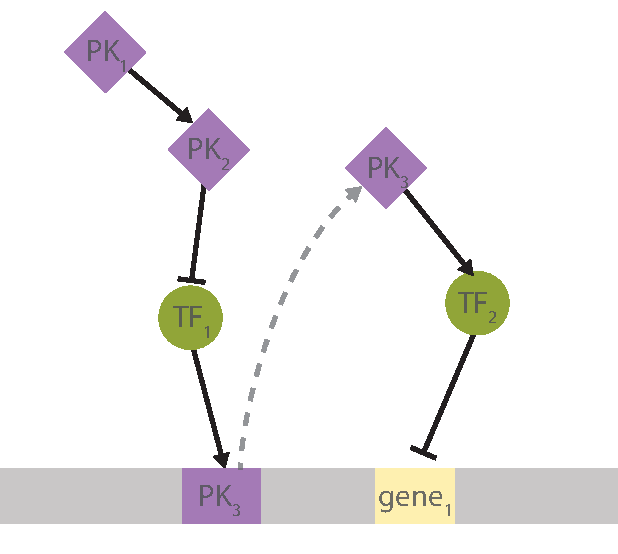
\includegraphics[width=0.7\textwidth]{introduction/fig/problem.pdf}
  \caption{\textbf{Gene regulation.}
  $\pk_1$ regulating $\gene_1$ indirectly through a cascade.}
  \label{fig:problem}
\end{figure}
\end{column}
\end{columns}
\end{frame}


\begin{frame}{Theoretical background}
\begin{columns}
\begin{column}{0.5\textwidth}
% In this section theory and models of gene regulation are discussed, with models used for different types of inference goals and varying assumptions. Relevant previous work leading to the analysis are covered.
Signal transduction
\begin{itemize}
    \item Phosphorylation
% Signal transduction inside the cell is mostly performed through the addition or removal of phosphates as phosphorylation or dephosphorylation of proteins, although there are many other types of signal transduction and protein regulation such as G-protein coupled receptors mediating trans-membrane signals, second messengers such as calcium ions and lipid messengers. 
    \item TF, $\text{KP} = \text{PK} \cup \text{PP}$, V (any genes)
% For intracellular signals leading to gene regulation, gene regulatory proteins can broadly be categorizes as either transcription factors, kinases or phosphatases, where the TFs have direct effects on the gene transcription and kinases and phosphatases regulates the activity of TFs as well as each other. TFs and their regulons, which are the set of genes regulated by a TF, are largely known, while kinase regulation is not as well documented.

% There are about a factor of 10 less phosphatases of yeast than kinases. They have a much smaller specificity in regulation targets and can, to some extent, be seen as serving a general clean-up role by removing phosphates from regulated proteins in order to let cellular signals decay.
% Phosphorylation can generally be seen as a on/off switch for a specific site on the protein, with one state of phosphorylation inducing an active conformation while the other stabilizes a more inactive conformation. It is atypical that a transcription factor will regulate one set of genes while phosphorylated and another while dephosphorylated. It can both be a phosphorylation that activates a proteins function or deactivates it, however since kinases have more specificity, kinase chains will often send a cellular signal when phosphorylated and have the signal decay with dephosphorylation mediated by phosphatases. Proteins are often modeled as either being on or off, but multiple post-translational modifications can have combined effects leading to multiple levels of protein activity for a given protein.
\end{itemize}

Mutant RNA measurements
\begin{itemize}
    \item Gene deletions reveal indirect insight
% indirect insight
    % Gene deletion, or knockouts, can reveal insight into gene regulation even through RNA expression measurements are not a direct assay for protein-DNA or protein-protein interactions.
% figure
    % If the gene expression levels are observed relative to wildtype we can observe how a gene's expression is affected by the presence or absence of a regulator~(\autoref{fig:gene_deletion}). The direct regulation effects of transcription factors are more straightforward than the indirect effects of a protein kinase. Both edges cannot be inferred from any single knockout experiment even for this simple regulation example. By combining the observation in both an experiment with PK deleted and another with the TF deleted the signs of both edges can be determined, where +1 symbolizes activation and -1 repression. In this manner we can infer edges based on gene expression levels observed to be significantly up- or downregulated compared to wildtype in each of these four patters. The example here is simplified to not include any other regulators which can complicate the edge inference, e.g. if there is another regulation pathway that works as a backup for transcription of the regulated gene, so a robust inference method cannot be basing inference on individual regulation paths in isolation.
    
    \item Vital genes
% A protein chosen to be knocked out might be vital to the functioning of the cell, making it impossible to have any mutant cells to observe. When this is the case a researcher can apply a conditional knockout where the gene can be down-regulated in a time-dependent manner so the measurements can be gathered at a specific time after inducing the knockout and before the death of all cells.

% genes where the mutant is not visibly different than wildtype due to low expression of the gene under the tested conditions
% \textbf{Low wildtype expression at tested conditions}

% There can be issues with genes expressed at low levels in the wildtype under the experimental conditions. If the expression is already low for the wildtype it can be difficult to tell the level apart in a knockout mutant given the noise of microarray measurements. For this reason it has been argued~\cite{ChuaPNAS2006} that overexpression of transcription factors is better than knockouts for transcription factors that might not be expressed at the tested environmental conditions. According to their tests overexpression is good enough to produce noticeable changes even for some transcription factors that would normally not be active under the tested environmental conditions.
% A counterpoint can be made with Savageau’s rule of demand~(\autoref{sec:demand_rule}).

    \item Savageau's rule of demand~\cite{Shinar2006}
\label{sec:demand_rule}
% We consider Savageau’s rule of demand which states that high demand genes are generally induced, and low demand genes repressed under typical conditions. Another way of phrasing it is that genes are bound by their regulators at most times. The rule is established empirically as well as from the evolutionary intuition that it creates the highest selection pressure against unfavorable mutations~\cite{Shinar2006}. If it was the opposite case, where genes were generally not bound by their regulators under typical conditions, a mutation of a regulator could have a less noticeable effect. 
\begin{itemize}
    \item KOs are noticeable
% If Savageau's rule of demand holds, a transcription factor will most likely not be expressed at a near undetectable level under typical conditions, so we would expect a knockout of said TF to have a noticeable effect. In the case of overexpression experiments the expression levels will be noticeably different from wildtype if the transcription is not already saturating the target gene promotor. That will typically not be the case for activating TFs where there would be a 2 to 4 fold increase in expression, but in the case of repressors the promotor can be close to saturated and the effect of TF overexpression can be harder to detect.

% If Savageau's rule of demand does \textit{not} hold, so the promotor of a gene is more often bound by a TF under atypical conditions, it will be harder to detect deviation from wildtype expression levels when the TF is under- or overexpressed. TFs responding to stress and alternative carbon sources and their regulons appear to often violate Savageau’s demand rule so their regulation could be missed if not studied under the appropriate conditions.
\end{itemize}
\end{itemize}



\end{column}
\begin{column}{0.5\textwidth}
\begin{figure}[ht]
    \centering
    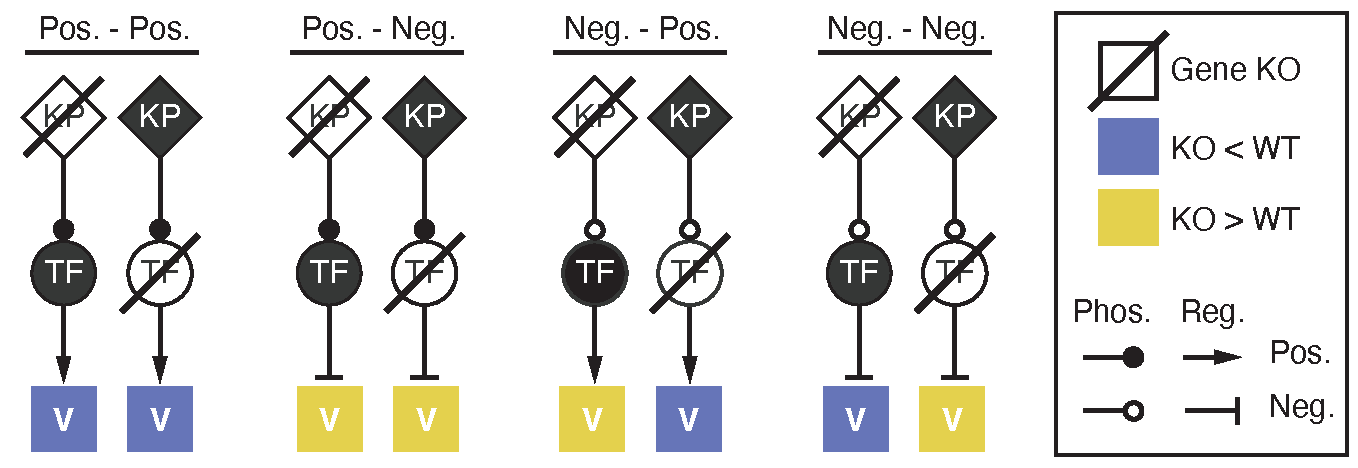
\includegraphics[width=\textwidth]{introduction/fig/Fig1.pdf}
    \caption{\textbf{Effects of gene deletion on gene expression.} Schematic of gene expression levels for a target gene ’V’ relative to wildtype when a gene for either a PK or TF is deleted. All combinations of positive (activating) and negative (repressing) regulation (Pos. or Neg. respectively) are shown. Activating or repressing phosphorylation (Phos.) are indicated with closed or open circles and regulation by TFs (Reg.) are indicated with pointed and flat arrowheads.}
    \label{fig:gene_deletion}
\end{figure}
\end{column}
\end{columns}
\end{frame}





\section{Simulation}
\subsection{Modelling gene expression with differential equations}
\begin{frame}{Modelling gene expression with differential equations}
% Transcription and translation kinetics are often modelled using differential equations~\cite{Chen99}. We can model the dynamic as~\autoref{eq:Chen99}, if we assume the process of transcription and translation takes a negligible amount of time, so the effect of regulation becomes instantly apparent in the rates of molecule production.
Chen et al.~\cite{Chen99}
\begin{subequations}
\label{eq:Chen99}
\begin{align}
\dv{\boldsymbol{r}}{t} &=
f(\boldsymbol{p}) - \Lambda_\text{RNA} \boldsymbol{r}
\\
\dv{\boldsymbol{p}}{t} &=
M \boldsymbol{r} - \Lambda_\text{Prot} \boldsymbol{p}
\end{align}
\end{subequations}
% Here, $\boldsymbol{r}$ is a vector of mRNA concentrations $r_i$ for each gene $i$, $\boldsymbol{p}$ is similarly a vector of protein concentrations for each gene $i$. $\Lambda_\text{RNA}$ and $\Lambda_\text{Prot}$ are diagonal matrices holding decay rates for each mRNA or protein, $M$ is a matrix with values for linear rates of protein production from the relevant coding mRNA, and $f$ is some function for how mRNA rates are influenced by each of the protein concentrations. Chen~et~al. argues for the application of using $f(\boldsymbol{p}) = C \boldsymbol{p}$ with a Taylor approximation and defines the solution to the ordinary linear system of differential equations. 

% Differential models describing time-dependent kinetics of transcription and translation regulation can be readily applied to time series data. It can be done by assuming that the intervals between measurements are short enough that the differential can be approximated with the differences between measurements at each time step, however real-time measurements are collected at a lower rate than the time scale of biological interaction.

% Differential equations has been used for modelling gene regulation with multiple transcription factors with both linear and nonlinear gene regulation, for instance by Anderson~et~al.~\cite{Anderson2009}, who modeled transcription factor concentrations as Gaussian Processes which are stochastic processes, purely defined by a mean and covariance term~(\autoref{eq:gaussian_process}).
Gaussian Processes~\cite{Anderson2009}
\begin{subequations}
\label{eq:gaussian_process}
\begin{align}
\dv{\boldsymbol{r}}{t} &=
\boldsymbol{r}_0 + C \boldsymbol{p} - \Lambda_\text{RNA} \boldsymbol{r}
\\
p_i &= f_i(t) =
\mathcal{GP}\left(0, \exp(-\frac{(t-t')^2}{l_i^2})\right)
\end{align}
\end{subequations}
\begin{itemize}
% Here, $\boldsymbol{r}_0$ is a vector with basal transcriptional concentrations for each gene, $p_i$ is the $i$-th element of the protein concentration vector $\boldsymbol{p}$ which describes the concentrations of transcription factors as a Gaussian Process $\mathcal{GP}$ with mean 0 and covariance as an exponential function. $l_i$ is a hyperparameter of the model, which was chosen to be 0.1 for one example of simulation. Modelling the transcription factors as a Gaussian Process leaves out regulatory effects onto transcription factors, so the model was further extended to describe a cascade of transcription factors, each regulating the gene of the next transcription factor in the cascade. The models were not extended to protein kinases. 
    \item \textcolor{darkgray!50!gray}{models for time series gene expression $\rightarrow$ GP parameters}
% The models are in this case used for inferring the parameters defining the underlying Gaussian Processes for the transcription factor concentrations, that were giving rise to the observed gene transcription levels. It assumes adequate amounts of time series data for the gene transcripts, and does not directly infer which transcription factors regulate which genes, but rather assumes it is known.
    \item \textcolor{darkgray!50!gray}{intentions of generalization, using TF concentration $\rightarrow$ TF interactions}
% If the model could be generalized to describing any combination of transcription factors and designed to utilize TF concentrations, it might be possible to infer which transcription factor interactions are present. 
\end{itemize}
\end{frame}

% \subsubsection{GeneNetWeaver}
\begin{frame}<1>[label=gnw]
\label{sec:dream}
\begin{columns}
\begin{column}{0.53\textwidth}
\alt<1>{
\frametitle{GeneNetWeaver}
\begin{itemize}
    \item Simulating gene expression in Java
    \item Used in DREAM challenge for benchmarking inference
    \item Regulation model:
\end{itemize}
% Modelling gene expression with differential equations has been applied to benchmark different attempts at inferring which transcription factors regulate which genes. The DREAM~(Dialogue for Reverse Engineering Assessments and Methods) challenges are organised by a variety of researchers from multiple organizations putting forward a challenge open to the public and assessing attempts at a solution. "DREAM4" was a challenge in reverse-engineering an in silico gene regulation network from gene expression levels. Gene expression levels were simulated, instead of collected experimentally, in order for the true underlying interactions to be definitively known.
% The simulation was intended to be biologically realistic and was simulated using the Java software GeneNetWeaver applying a nondimensionalized model defined as the differential equations in~\autoref{eq:gnw_main}, which are clearly similar to the differential equations in~\autoref{eq:Chen99}.
\begin{subequations}
\label{eq:gnw_main}
\begin{align}
\label{eq:gnw_main.a}
\dv{r_i}{t} &=  m_i^{(\text{RNA})} f_i(\boldsymbol{p}) - \lambda_i^{(\text{RNA})} r_i \\
\dv{p_i}{t} &=  m_i^{(\text{Prot})} r_i -  \lambda_i^{(\text{Prot})} p_i
\end{align}
\end{subequations}
% The values $m_i^{(\text{RNA})}$ and $m_i^{(\text{Prot})}$ are the maximum transcription and translation levels for the $i$-th protein. The function $f_i$ describes the expected fraction of maximum transcription for gene $i$ given nondimensionalized protein concentrations $\boldsymbol{p}$, so it holds $f_i(\boldsymbol{p}) \in [0,1]$.
% $f_i$ is mentioned in supplementary material of~\cite{Marbach2010} and based on the work in~\cite{GeneNetWeaverModel}. It takes into account different types of gene regulation, both regulator interactions and cooperation for any combination of activators and repressors~(\autoref{fig:gnw_regulation}).
% A gene has a set of binding sites, each affecting its transcription level. Each of the TFs regulating gene $i$ can bind to only one binding site in the GeneNetWeaver model. The TF can bind to the binding site with dynamics built on Hill equations~(\autoref{eq:Hill}). The effect of a bound site on gene transcription rate can be flipped in the model, indicated for site $m=2$ in~\autoref{fig:gnw_regulation}, where TFs binding the site using dynamics inspired by activator Hill equations~(\autoref{eq:Hill_activator}) has a repressing effect on the transcription rate of gene $i$.
}{
\stepcounter{equation}
}
\only<2>{
\frametitle{GeneNetWeaver - Example}
% The terms defined in~\autoref{eq:gnw_f} are calculated using the example shown in~\autoref{fig:gnw_regulation} for illustrative purposes:
\begin{subequations}
\begin{align*}
N &= 3
\,,\,
C = \{3\}
\\
A_1 &= \{1\}
\,,\,
A_2 = \{4\}
\,,\,
A_3 = \{5,6\}
\\
R_1 &= \emptyset
\,,\,
R_2 = \{2,3\}
\,,\,
R_3 = \emptyset
\\
\mu_1 &= \frac{\chi_1}{1 + \chi_1}
\\
\mu_2 &= \frac{\chi_4}{1 + \chi_4 + \chi_2 \chi_3 \chi_4}
\\
\mu_3 &= \frac{\chi_5}{1 + \chi_5} \frac{\chi_6}{1 + \chi_6}
\\
\sigma_1 &= \emptyset
\,,\,
\sigma_2 = \{1\}
\,,\,
\sigma_3 = \{2\}
\,,\,
\sigma_4 = \{1,2\}
\\
\sigma_5 &= \{3\}
\,,\,
\sigma_6 = \{1,3\}
\,,\,
\sigma_7 = \{2,3\}
\,,\,
\sigma_8 = \{1,2,3\}
\\
P\{\sigma_1 | \boldsymbol{p}\} &= (1 - \mu_1) (1 - \mu_2) (1 - \mu_3)
\\
P\{\sigma_2 | \boldsymbol{p}\} &= \mu_1 (1 - \mu_2) (1 - \mu_3)
\\
P\{\sigma_3 | \boldsymbol{p}\} &= (1 - \mu_1) \mu_2 (1 - \mu_3)
\\
...
\\
P\{\sigma_8 | \boldsymbol{p}\} &= \mu_1 \mu_2 \mu_3
\end{align*}
\end{subequations}

}
\end{column}
\begin{column}{0.47\textwidth}

\begin{figure}[ht]
  \centering
  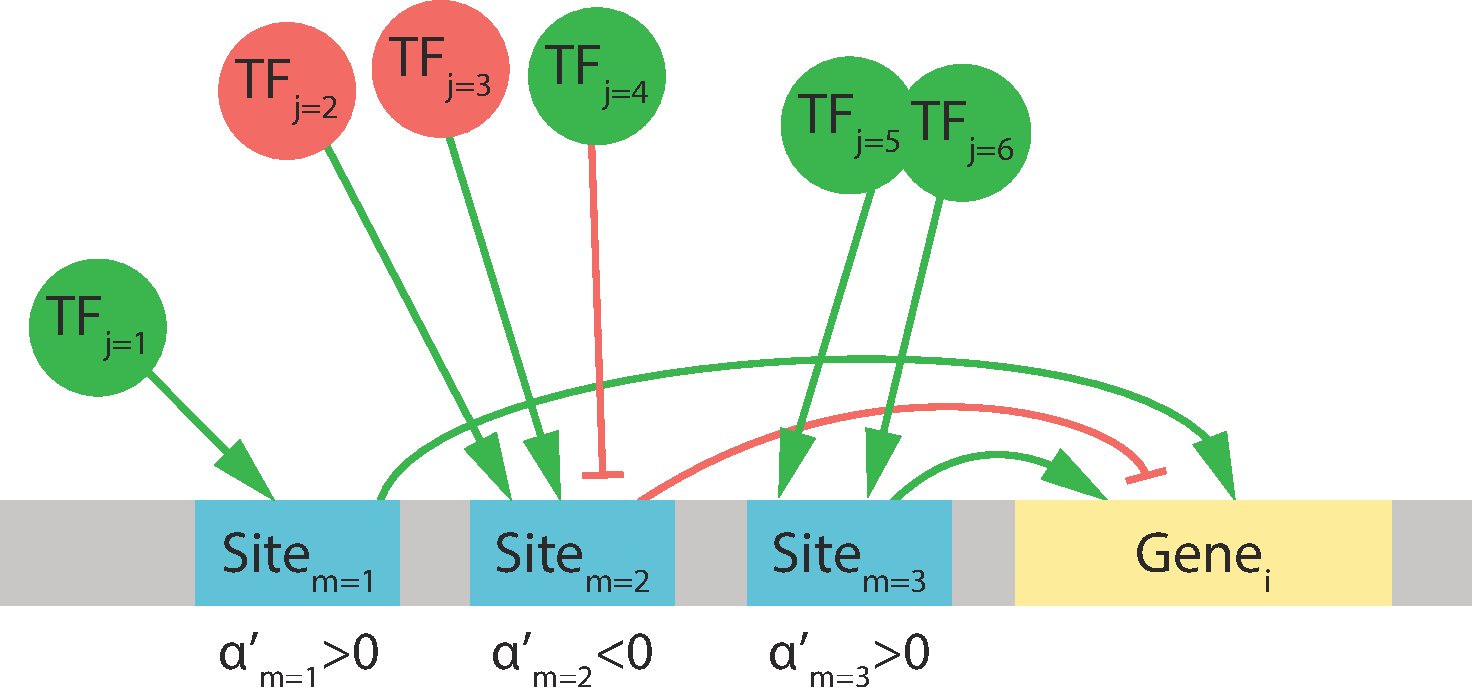
\includegraphics[width=\textwidth]{theory/fig/GeneWeaverRegulation.pdf}
   \caption{\textbf{Example of transcriptional regulation in simulation.}
    A gene regulated by $N=3$ regulatory modules, where module 1 is regulated by a single activator TF, module 2 is bound by a complex of two TFs, which both have to be present for activation of the module, and activating and repressing TFs compete to bind the third module. \textcolor{OliveGreen}{Green}: activation, \textcolor{red}{red}: repression.} 
  \label{fig:gnw_regulation}
\end{figure}



\end{column}
\end{columns}
\end{frame}


\begin{frame}{Modelling cooperativity}
\begin{columns}
\begin{column}{0.4\textwidth}
% For the simple case of a single transcription factor regulating the transcription rate of a single gene, the number of protein molecules produced of the regulated gene per unit time is a function of the concentration of the transcription factor in its active form~\cite{Alon2006}.
% The Hill equations~(\autoref{eq:Hill}) describe the cooperativity of binding for ligands to a receptor or for a similar binding event, for instance the binding of TFs to a regulatory region of DNA. The Hill equation is given here for the case of a single activator~(\autoref{eq:Hill_activator}) and a single repressor~(\autoref{eq:Hill_repressor}).
Single transcription factor regulating a single gene~\cite{Alon2006}
\begin{subequations}
\label{eq:Hill}
\begin{align}
\label{eq:Hill_activator}
\theta_{\text{activator}} &= \frac{p_j^{\nu_j}}{k_j^{\nu_j} + p_j^{\nu_j}} = \frac{\chi_j}{1 + \chi_j}
\\
\label{eq:Hill_repressor}
\theta_{\text{repressor}} &= \frac{1}{1 + \left(\frac{p_j}{k_j} \right)^{\nu_j}} = \frac{1}{1 + \chi_j}
\\
\chi_j &=
\left( \frac{p_j}{k_j} \right) ^ {\nu_j}
\end{align}
\end{subequations}
% Here $p_j$ is the ligand concentration (concentration of the $j$-th protein), $k_j$ and $\nu_j$ are model parameters. Different values for $k_j$ and the Hill coefficient $\nu_j$ determines $\theta$, which is the fraction of maximum transcription if regulated by either a single activator or repressor. If the concentration of ligand is $p_j = k_j$ then there will be half occupancy of the receptor. The basic assumption is that we use the fraction of occupancy of bound receptor~(the promotor of a gene), to describe transcription rate. The equations are sometimes multiplied by a constant $r_\text{max}$, which holds the maximum transcription rate unique to a given gene. This way $\theta$ will be the absolute instead of relative transcription rate, and have the dimension of $r_\text{max}$ instead of being dimensionless.


\end{column}
\begin{column}{0.6\textwidth}
\begin{figure}[ht]
\centering
\begin{subfigure}[b]{0.49\textwidth}\centering\caption{}
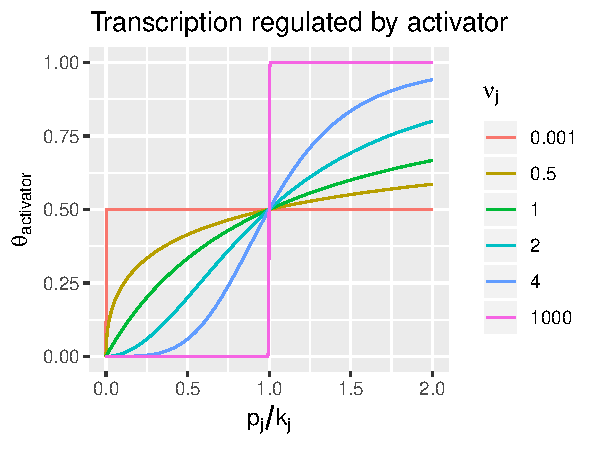
\includegraphics[width=\textwidth]{theory/fig/hill_activator.pdf}
\end{subfigure}
% \vskip\baselineskip
\begin{subfigure}[b]{0.49\textwidth}\centering\caption{}
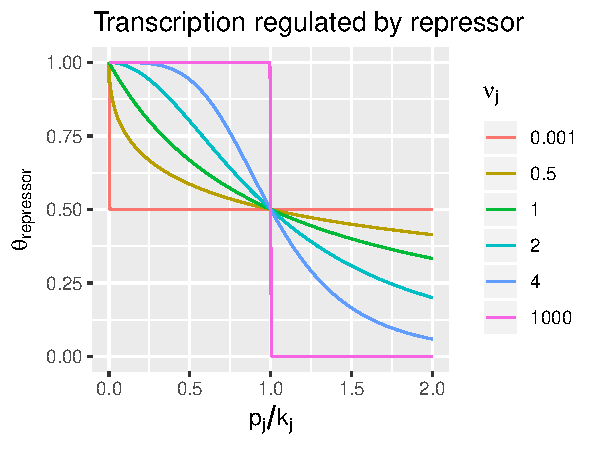
\includegraphics[width=\textwidth]{theory/fig/hill_repressor.pdf}
\end{subfigure}
\caption{\textbf{Hill equation models of gene regulation.} Single activator~(a), and repressor~(b).
% Unique curves result from using different model parameters $\nu_j$. 
}
\label{fig:Hill}
\end{figure}
% The equations are designed to capture cooperation in ligand binding as well as a receptor becoming saturated with increased ligand concentration~(\autoref{fig:Hill}).
% $\nu_j=1$ means that the receptor gets saturated linearly, $\nu_j<1$ means negative cooperation where it is more resistant to binding of ligand if some is already bound, and $\nu_j>1$ is positive cooperation. 
\end{column}
\end{columns}
\end{frame}



\begin{frame}{GeneNetWeaver - Defining gene regulation}
\begin{columns}
\begin{column}{0.5\textwidth}
% The exact equation for $f$ is unpublished but defined in the source code, and written here in~\autoref{eq:gnw_f}, focusing on the function $f_i$ for a single gene $i$. Each binding site can either be bound by transcription factor(s) or unbound. For $N$ binding sites this creates $2^N$ unique combinations~(\autoref{eq:gnw_f.a}), which we refer to as "states". Each state~$\sigma_s$ for $s \in \{1,2,3,...,2^N\}$ are each defined as a unique combination of bound and unbound binding sites.
\small
Based on Marbach~et~al.~\cite{Marbach2010}, Dassow~et~al.~\cite{GeneNetWeaverModel}
\normalsize
\begin{subequations}
\label{eq:gnw_f}
\begin{align}
\label{eq:gnw_f.a}
f_i(\boldsymbol{p}) &=
\sum_{s=1}^{2^N} \alpha_s P\{S = s | \boldsymbol{p} \}
\\
\label{eq:gnw_f.b}
\alpha_s &=
\alpha_0' + \sum_{m \in \sigma_s} \alpha_m'
\\
\label{eq:gnw_f.c}
P\{S = s | \boldsymbol{p} \} &=
\prod_{m \in \sigma_s} P\{\beta_m=1|\boldsymbol{p}\} \cdot \prod_{m \notin \sigma_s} \left( P\{\beta_m=0|\boldsymbol{p}\} \right)
\\
\label{eq:gnw_f.d}
&=
\prod_{m \in \sigma_s} \mu_m \cdot \prod_{m \notin \sigma_s} \left( 1 - \mu_m \right)
\end{align}
\end{subequations}
$\beta_m$ = module $m$ under activating binding conditions
\end{column}

\begin{column}{0.5\textwidth}
\begin{subequations}
\begin{align}
\label{eq:gnw_f.e}
\mu_m &=
\begin{cases}
  \frac{\prod_{j \in A_m} \chi_j}{\prod_{j \in A_m \cup R_m} 1 + \chi_j},
  & \text{if}\ m \notin C \\
  \frac{\prod_{j \in A_m} \chi_j}{1 + \prod_{j \in A_m} \chi_j},
  & \begin{aligned}
      &\text{if}\ m \in C \\ &\wedge R_m = \emptyset
  \end{aligned} \\
  \frac{\prod_{j \in A_m} \chi_j}{1 + \prod_{j \in A_m} \chi_j + \prod_{j \in A_m \cup R_m} \chi_j},
  & \text{otherwise}
\end{cases}
\\
\label{eq:gnw_f.f}
\chi_j &=
\left( \frac{p_j}{k_j} \right) ^ {\nu_j}
\end{align}
\end{subequations}
% Here, $P\{\sigma_s | \boldsymbol{p}\}$ is the probability that a gene is in regulation state $\sigma_s$ given the current protein concentrations $\boldsymbol{p}$. $\alpha_s$ is the fraction of maximum gene transcription for state~$\sigma_s$, and is computed from the sum of baseline activation and relative activation for each binding site that are bound in the given state $\sigma_s$~(\autoref{eq:gnw_f.b}). It holds $\alpha_s \in [0,1]$.
% If we consider state $\sigma_s$ a set of all binding sites bound when a gene is in said state, then the probability that gene $i$ is in state $\sigma_s$ is defined by the probability of sites in set $\sigma_s$ bound and sites not in $\sigma_s$ unbound~(\autoref{eq:gnw_f.c}). The Boolean $\beta_m$ indicates if site $m$ is bound or not. The probabilities are equivalent to the expected fraction of binding sites bound~(\autoref{eq:gnw_f.d}), which is defined in three different ways in~\autoref{eq:gnw_f.d} depending on whether the binding site is regulated by a TF binding complex~($m \in C$), and if some of the TFs for a binding site are repressors~($\exists j \in R_m$) or if all are activators~($\forall j \in A_m$).
% \autoref{eq:gnw_f.e} is based on Hill equations~(\autoref{eq:Hill}). It can be seen that if a binding site $m$ is only regulated by a single activating TF, then we get $\mu_m = \theta_{\text{activator}}$ from \autoref{eq:Hill_activator} and if only regulated by a single repressing TF, we get $\mu_m = \theta_{\text{repressor}}$ for \autoref{eq:Hill_repressor}. This is the case regardless if $m \in C$ or not, although it does not make sense to describe a lone transcription factor as regulating in a complex.
% \pagebreak
\end{column}
\end{columns}
\end{frame}

\againframe<2>{gnw}

\begin{frame}{GeneNetWeaver - Initial conditions}
% To prepare for the simulation, the GeneNetWeaver software is given an adjacency matrix~(\autoref{sec:graph}) with values indicating which genes each protein regulates. Model parameters are then set randomly, for instance setting random mRNA and protein decay rates. Rate parameters are assigned random values using~\autoref{eq:gnw_param_initial} which describes random decay rates.

\begin{subequations}
\label{eq:gnw_param_initial}
\begin{align}
m_i^{(\text{RNA})} &= \lambda_i^{(\text{RNA})} \sim \frac{\log (2)}{\mathcal{T}(a=5, b=50)} \\
m_i^{(\text{Prot})} &= \lambda_i^{(\text{Prot})} \sim \frac{\log (2)}{\mathcal{T}(a=5, b=50)}
\end{align}
\end{subequations}

$\mathcal{T}(a,b)$ = normal distribution truncated to $[a,b]$. $a$ and $b$ selected from~\cite{GeneNetWeaverModel}


$\mathcal{T}(a,b)$ has $\mu=\frac{a+b}{2}$, $\sigma=\frac{b-a}{6}$



% Here, $\mathcal{T}(a,b)$ is a normal distribution truncated to the interval $[a,b]$ with $\mu=\frac{a+b}{2}$ and $\sigma=\frac{b-a}{6}$. It serves as descriptor of mRNA and protein half-life. Its range parameters are selected based on~\cite{GeneNetWeaverModel}.


% Gene expression and protein levels are initialized at time zero by letting gradients equal zero as described in~\autoref{eq:initial_gnw}.

\begin{subequations}
\label{eq:initial_gnw}
\begin{align}
\dv{r_i}{t} = 0 &\implies r_i = \frac{m_i^{(\text{RNA})}}{\lambda_i^{(\text{RNA})}}  f_i(\boldsymbol{p})  \\
\dv{p_i}{t} = 0 &\implies p_i = \frac{m_i^{(\text{Prot})}}{\lambda_i^{(\text{Prot})}} r_i
\end{align}
\end{subequations}

% Gene expressions $r_i$ for each gene $i$ are initially set without protein regulation, which means $r_i$ is evaluated here using $\boldsymbol{p} = \boldsymbol{0}$. More initialization code is also run in order to set $\alpha_s$ for each state.


\end{frame}

\begin{frame}{Kinase regulation model}
\label{sec:Heinrich}

\begin{columns}
\begin{column}{0.5\textwidth}


% Protein phosphorylation is a ubiquitous means of regulating protein activity controlled by protein kinases and phosphatases. Kinase cascades allows a signal from outside the cell to propagate into the nucleus via phosphorylation events as modelled by Heinrich~et~al.~\cite{Heinrich2002kinase}.

% The signal can be described as a single activated receptor sending a signal that decays with rate~$\lambda^{(\text{Receptor})}$, and where each protein kinase has a single protein kinase input~(\autoref{fig:kinase_cascade}). The change in phosphorylation of a kinase $i$ is modelled as follows:
Kinase cascade, each protein with single input~\cite{Heinrich2002kinase}
\begin{subequations}
\label{eq:kinase_cascade}
\begin{align}
\dv{\phi_i}{t} &=
    \tilde{w}_i \phi_{i-1} \tilde{\phi}_i - \lambda_i^{(\text{Phos})} \phi_i
\\
    &=
    w_i \phi_{i-1} \left(1 - \frac{\phi_i}{p_i}\right) - \lambda_i^{(\text{Phos})} \phi_i
\\
p_i &= \phi_i + \tilde{\phi}_i
\,,\,
w_i = \tilde{w}_i p_i
\end{align}
\end{subequations}

% Here, $\phi_i$ is the amount of phosphorylated protein $i$ and $\tilde{\phi}_i$ is the unphosphorylated amount. $w_i$ is the kinase rate of phosphorylation by phosphorylated protein $i-1$ on unphosphorylated protein $i$, and $\lambda_i^\text{Phos}$ is the decay rate of the phosphate group on protein $i$, which is controlled by the reaction of all the phosphatases in the cell with protein $i$. 
% It is assumed that a phosphorylation event is always an unphosphorylated kinase being phosphorylated by another kinase which itself is phosphorylated.

% The regulation generalizes to include the possibility of multiple inputs of regulation onto each protein kinase, which can be written with vector notations~(\autoref{eq:kinase_general}).

Generalized, any protein can affect any protein
\begin{subequations}
\label{eq:kinase_general}
\begin{align}
\dv{\phi_i}{t} &=
    \left( \sum_j w_{ij} \phi_j \right) \left(1 - \frac{\phi_i}{p_i}\right) - \lambda_i^{(\text{Phos})} \phi_i
\\
\label{eq:matrix_kinase}
\dv{\boldsymbol{\phi}}{t} &= (W \boldsymbol{\phi}) \left(1 - \frac{\boldsymbol{\phi}}{\boldsymbol{p}}\right) - \Lambda_\text{Phos} \boldsymbol{\phi}
\end{align}
\end{subequations}

% Here $w_{ij}$ is the regulation effect from node $j$ to $i$, which is a positive value. The division in~\autoref{eq:matrix_kinase} is an elementwise division.


\end{column}
% \begin{column}{0.5\textwidth}
% \begin{figure}
% \begin{minipage}[c]{0.42\textwidth}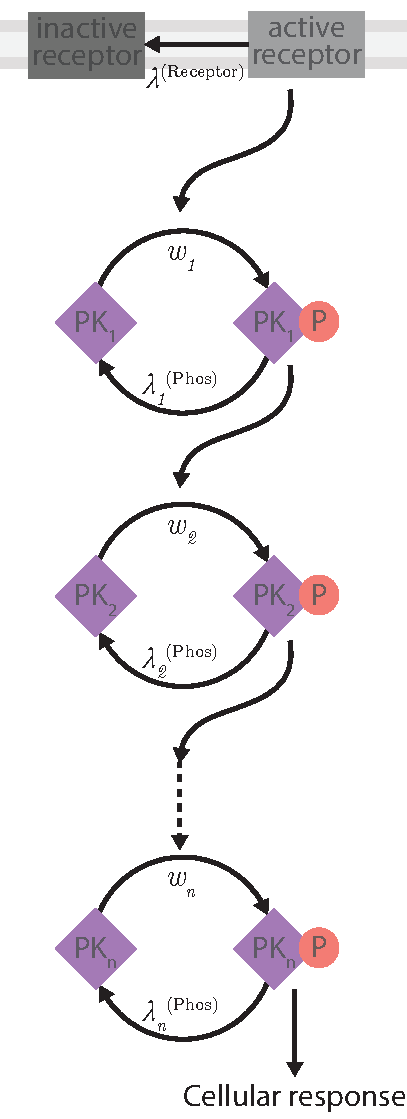
\includegraphics[width=\textwidth]{theory/fig/kinase_cascade.pdf}\end{minipage}
% \begin{minipage}[t]{0.54\textwidth}\caption{\textbf{Kinase cascade with single inputs.} A protein kinase cascade transmitting a signal from a cell membrane receptor.}\end{minipage}
% \label{fig:kinase_cascade}
% \end{figure}
% \end{column}

\begin{column}{0.5\textwidth}
\begin{figure}
\begin{minipage}[t]{0.4\textwidth}
\caption{\textbf{Kinase cascade with single inputs.} Transmitting signal from a membrane receptor.}
\end{minipage}
\begin{minipage}[c]{0.37\textwidth}
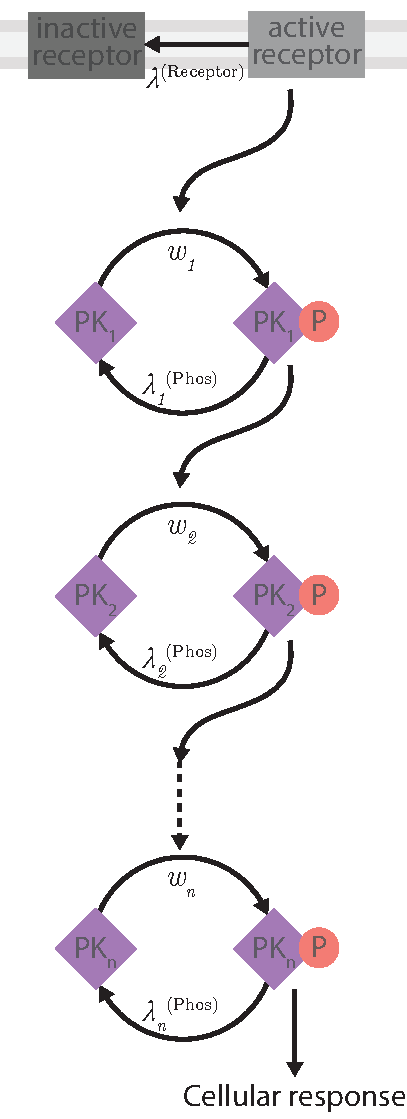
\includegraphics[width=\textwidth]{theory/fig/kinase_cascade.pdf}
\end{minipage}
\label{fig:kinase_cascade}
\end{figure}
\end{column}
\end{columns}
\end{frame}



\subsection{GeneNetWeaverPhos}
\begin{frame}{GeneNetWeaverPhos}
\label{sec:gnw_extension}
Java program GeneNetWeaver extended in Julia as GeneNetWeaverPhos. Added activated protein concentration, in some cases equal to phosphorylated concentration.
% GeneNetWeaver simulates gene expression levels for biological networks so network inference methods can systematically be benchmarked and compared.
% The software is not sufficient to benchmark a network inference method for indirect protein kinase interactions since the underlying simulation method is a gene regulation model only taking transcription factors into account.
% The program was extended to take indirect kinase effects into account in simulating the gene expression levels.
% The software is an open source Java program with a vast amount of features and built-in datasets. The core code was rewritten in Python to make the process of extending it as easy as possible.
% Code from \texttt{HillGene.java} was used for gene regulation, and initial conditions are described in \texttt{SteadyStateExperiment.java}. 
% The effects from kinases are added to the model with the differential equations in~\autoref{eq:gnw_kinase}, that based on the equations described in \autoref{sec:Heinrich}.
% The model described in \autoref{sec:dream} is extended by replacing the protein level terms $p_i$ with $y_i \cdot p_i$ describing the effective level of each protein instead of the total amount.
% The model of GeneNetWeaver is nondimensionalized, $p_i$ does not describe an absolute concentration but is relative to a maximum concentration. $y_i \cdot p_i$ is also nondimensionalized, since $y_i$ is unitless~(\autoref{eq:y_i}).
\begin{subequations}
\label{eq:gnw_kinase}
\begin{align}
\label{eq:dydt}
\dv{\boldsymbol{\psi}}{t} &= \left(W_{\text{KP}+} \boldsymbol{\psi}_\text{KP} + \boldsymbol{\lambda}_+\right) \left( \boldsymbol{p}_\text{TFKP} - \boldsymbol{\psi} \right) - \left(W_{\text{KP}-} \boldsymbol{\psi}_\text{KP} + \boldsymbol{\lambda}_- \right) \boldsymbol{\psi}
\end{align}
\end{subequations}
% Here, $\dv{\phi_i}{t}$ is found using \autoref{eq:kinase_general}.
% The values $y_i$ describe the phosphorylated fraction of protein $i$, so in this model it is assumed that the phosphorylated version of any protein is the active version. This is a simplification, but enough of an extension as a starting point to include effect of the kinases in the simulation.
% The differential equation \autoref{eq:dydt} is used as well as the already mentioned ones~(\autoref{eq:gnw_main}) for simulation of system until approximate convergence.
% The initial conditions is the same as for GeneNetWeaver with the addition of using $y_i = 0.5$ for all $i$. 
% RNA log fold-change measurements used as node values are simulated by solving the ODE at different times $t$ using the function \texttt{integrate.odeint} from the Python package \texttt{SciPy}. 
% Individual simulations are run using a wildtype network, as well as networks lacking nodes based on each of the experimental knockout conditions. For knockouts, a node $i$ is removed from the graph by setting the maximum transcription rate of gene $i$ to zero, which is $m_i^{(RNA)} = 0$~(\autoref{eq:gnw_main.a}).
% Log fold-change values are calculated for each of the modified networks relative to the wildtype measurements, after simulation completion. The last and second-to-last measurements are checked for approximate convergence with \autoref{eq:convergence} using threshold $\epsilon_{tol} = 0.005$. Warnings from the \texttt{odeint} call are also used in determination of successful convergence. The ODE is first solved for times $t \in \{0,1,...,9\}$, if this fails to converge it is solved for $t \in \{0,10,...,90\}$ and lastly for $t \in \{0,100,...,900\}$. If all fails the regulation modules are setup anew, as well as setting model parameters with new random values.
GeneNetWeaver $f$ changed from using $\boldsymbol{p}$ to $\boldsymbol{\psi}$.
\begin{subequations}
\begin{align}
\dv{r_i}{t} &=
m_i^{(\text{RNA})} f_i(\textcolor{red}{\boldsymbol{\psi}}) - \lambda_i^{(\text{RNA})} r_i
\end{align}
\end{subequations}
% $\odot$ = element-wise multiplication
\end{frame}


\begin{frame}{Small example network}
\begin{columns}
\begin{column}{0.4\linewidth}

(A) True network.\\
(B-F) Red = KO. Node value = Simulated mRNA logFC. Edge value = true weight.\\
(G) Total effects.\\
(H) Inferred edge weights.\\


\end{column}
\begin{column}{0.6\linewidth}
\begin{figure}[ht]
\centering
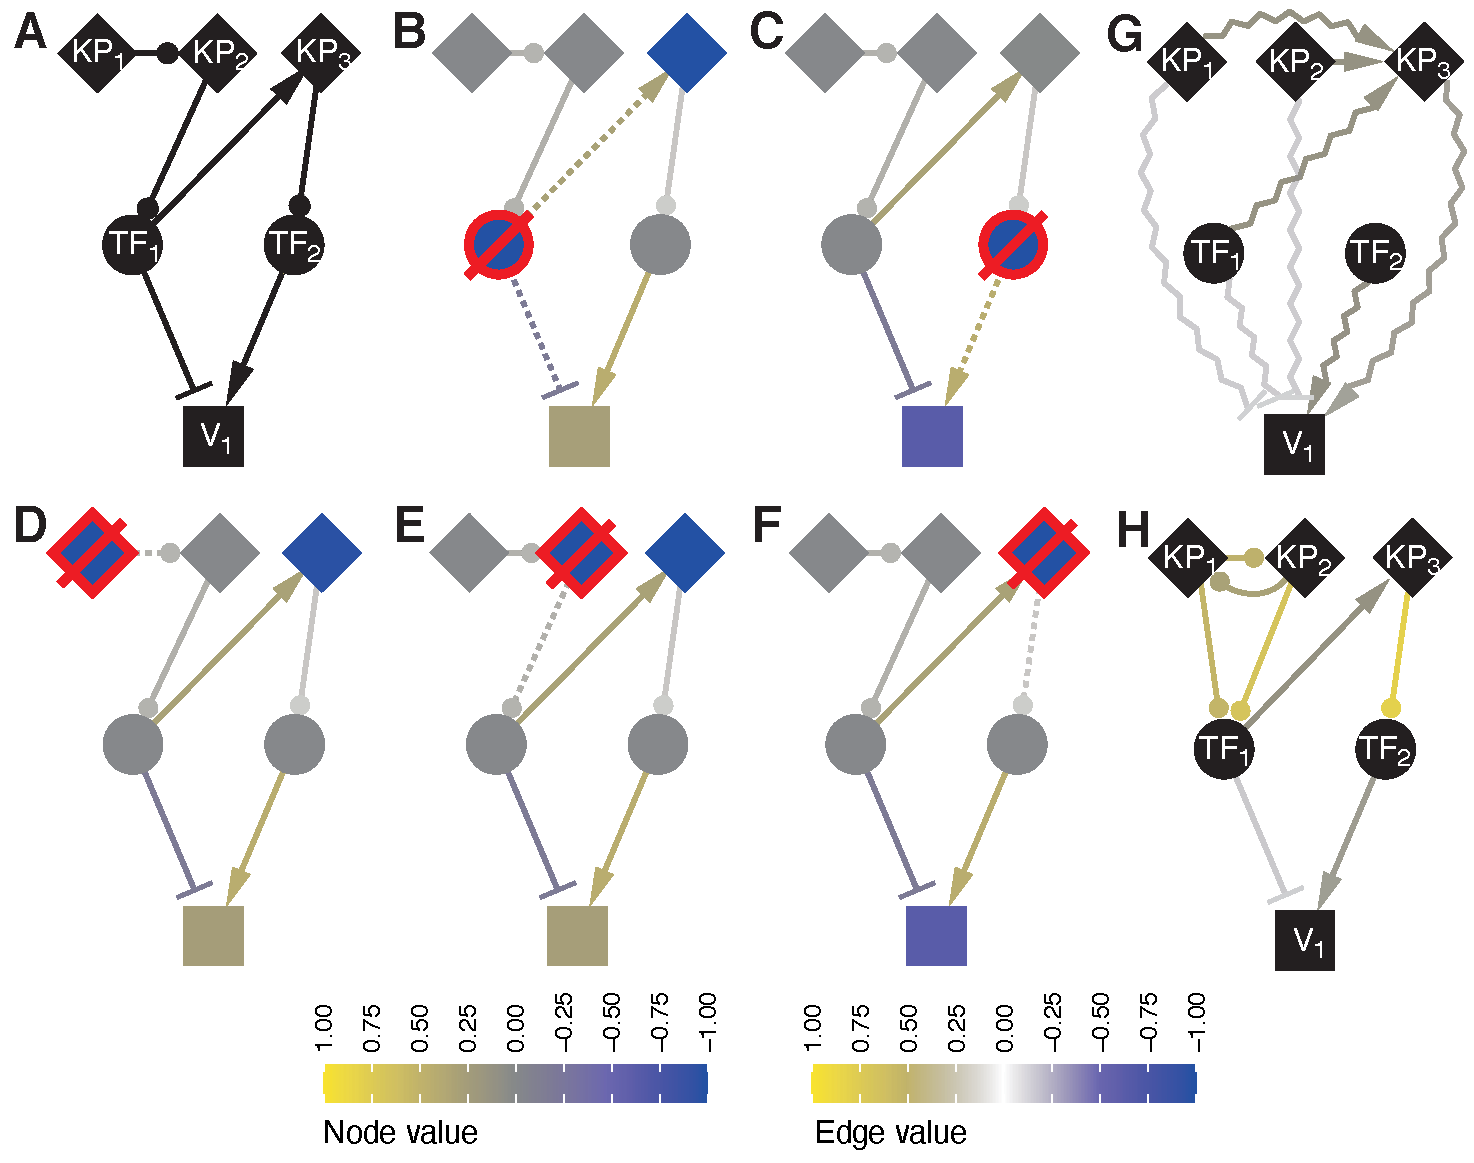
\includegraphics[width=\linewidth]{theory/fig/Fig2.pdf}
\caption{\textbf{Small example network with unresolvable ambiguity.}}
\label{fig:small}
\end{figure}
\end{column}
\end{columns}
\end{frame}


\begin{frame}{GeneNetWeaverPhos example}

\begin{columns}
\begin{column}{0.3\textwidth}
\end{column}
\begin{column}{0.7\textwidth}
\begin{figure}[ht]
    \centering
    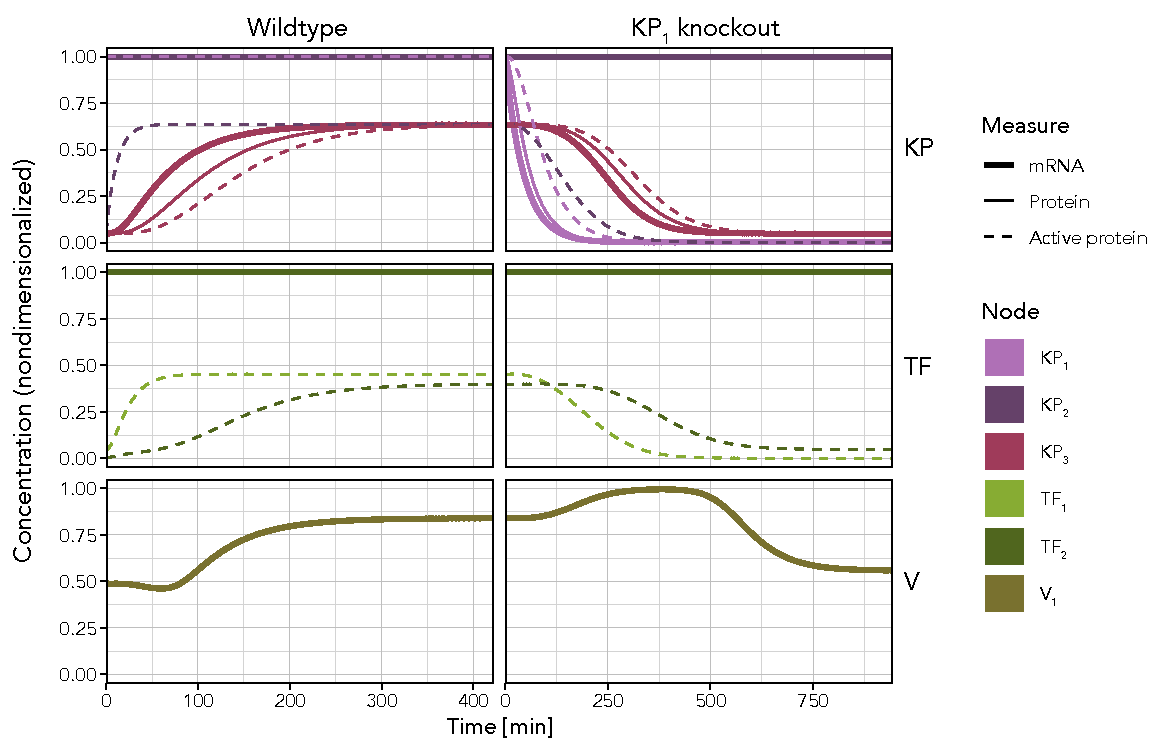
\includegraphics[width=\linewidth]{methods/fig/simulation_KP1_v4.pdf}
    \caption{{\bf Simulation until steady state.}
    Simulation of network in Fig~\ref{fig:small} in the main~text until convergence. 
    Comparing wildtype and a mutant where $\text{KP}_1$ has been knocked out. The values at convergence are seen in Fig~\ref{fig:small}D.
    }
     \label{fig:simulation}
\end{figure}
\end{column}
\end{columns}

\end{frame}


\subsection{DREAM challenge networks}
\begin{frame}<1-2>{DREAM challenge networks}
\label{sec:dream_data}
\begin{columns}
\begin{column}{0.4\textwidth}
% From DREAM challenge "DREAM4" 5 networks were available of 10 nodes each~(\autoref{fig:dream4_nets10}) as well as 5 networks of 100 nodes~(\autoref{fig:dream4_nets100})~\cite{dream4}. Networks with 10 nodes are referred to as 10.x and with 100 nodes named 100.x where x is in range~$[1,5]$.
DREAM4 simulated data~\cite{dream4}:
\begin{itemize}
    \item RNA expression at equilibrium for WT, single knockouts and knockdowns
    \item RNA expression at equilibrium for dual knockouts, and indexes of the knocked out genes
    \item time-series of RNA expression for single knockouts
    \item "gold standard" true edges
\end{itemize}
\end{column}

\begin{column}{0.6\textwidth}
\alt<1| handout:1>{
\begin{figure}[ht]
    \centering
    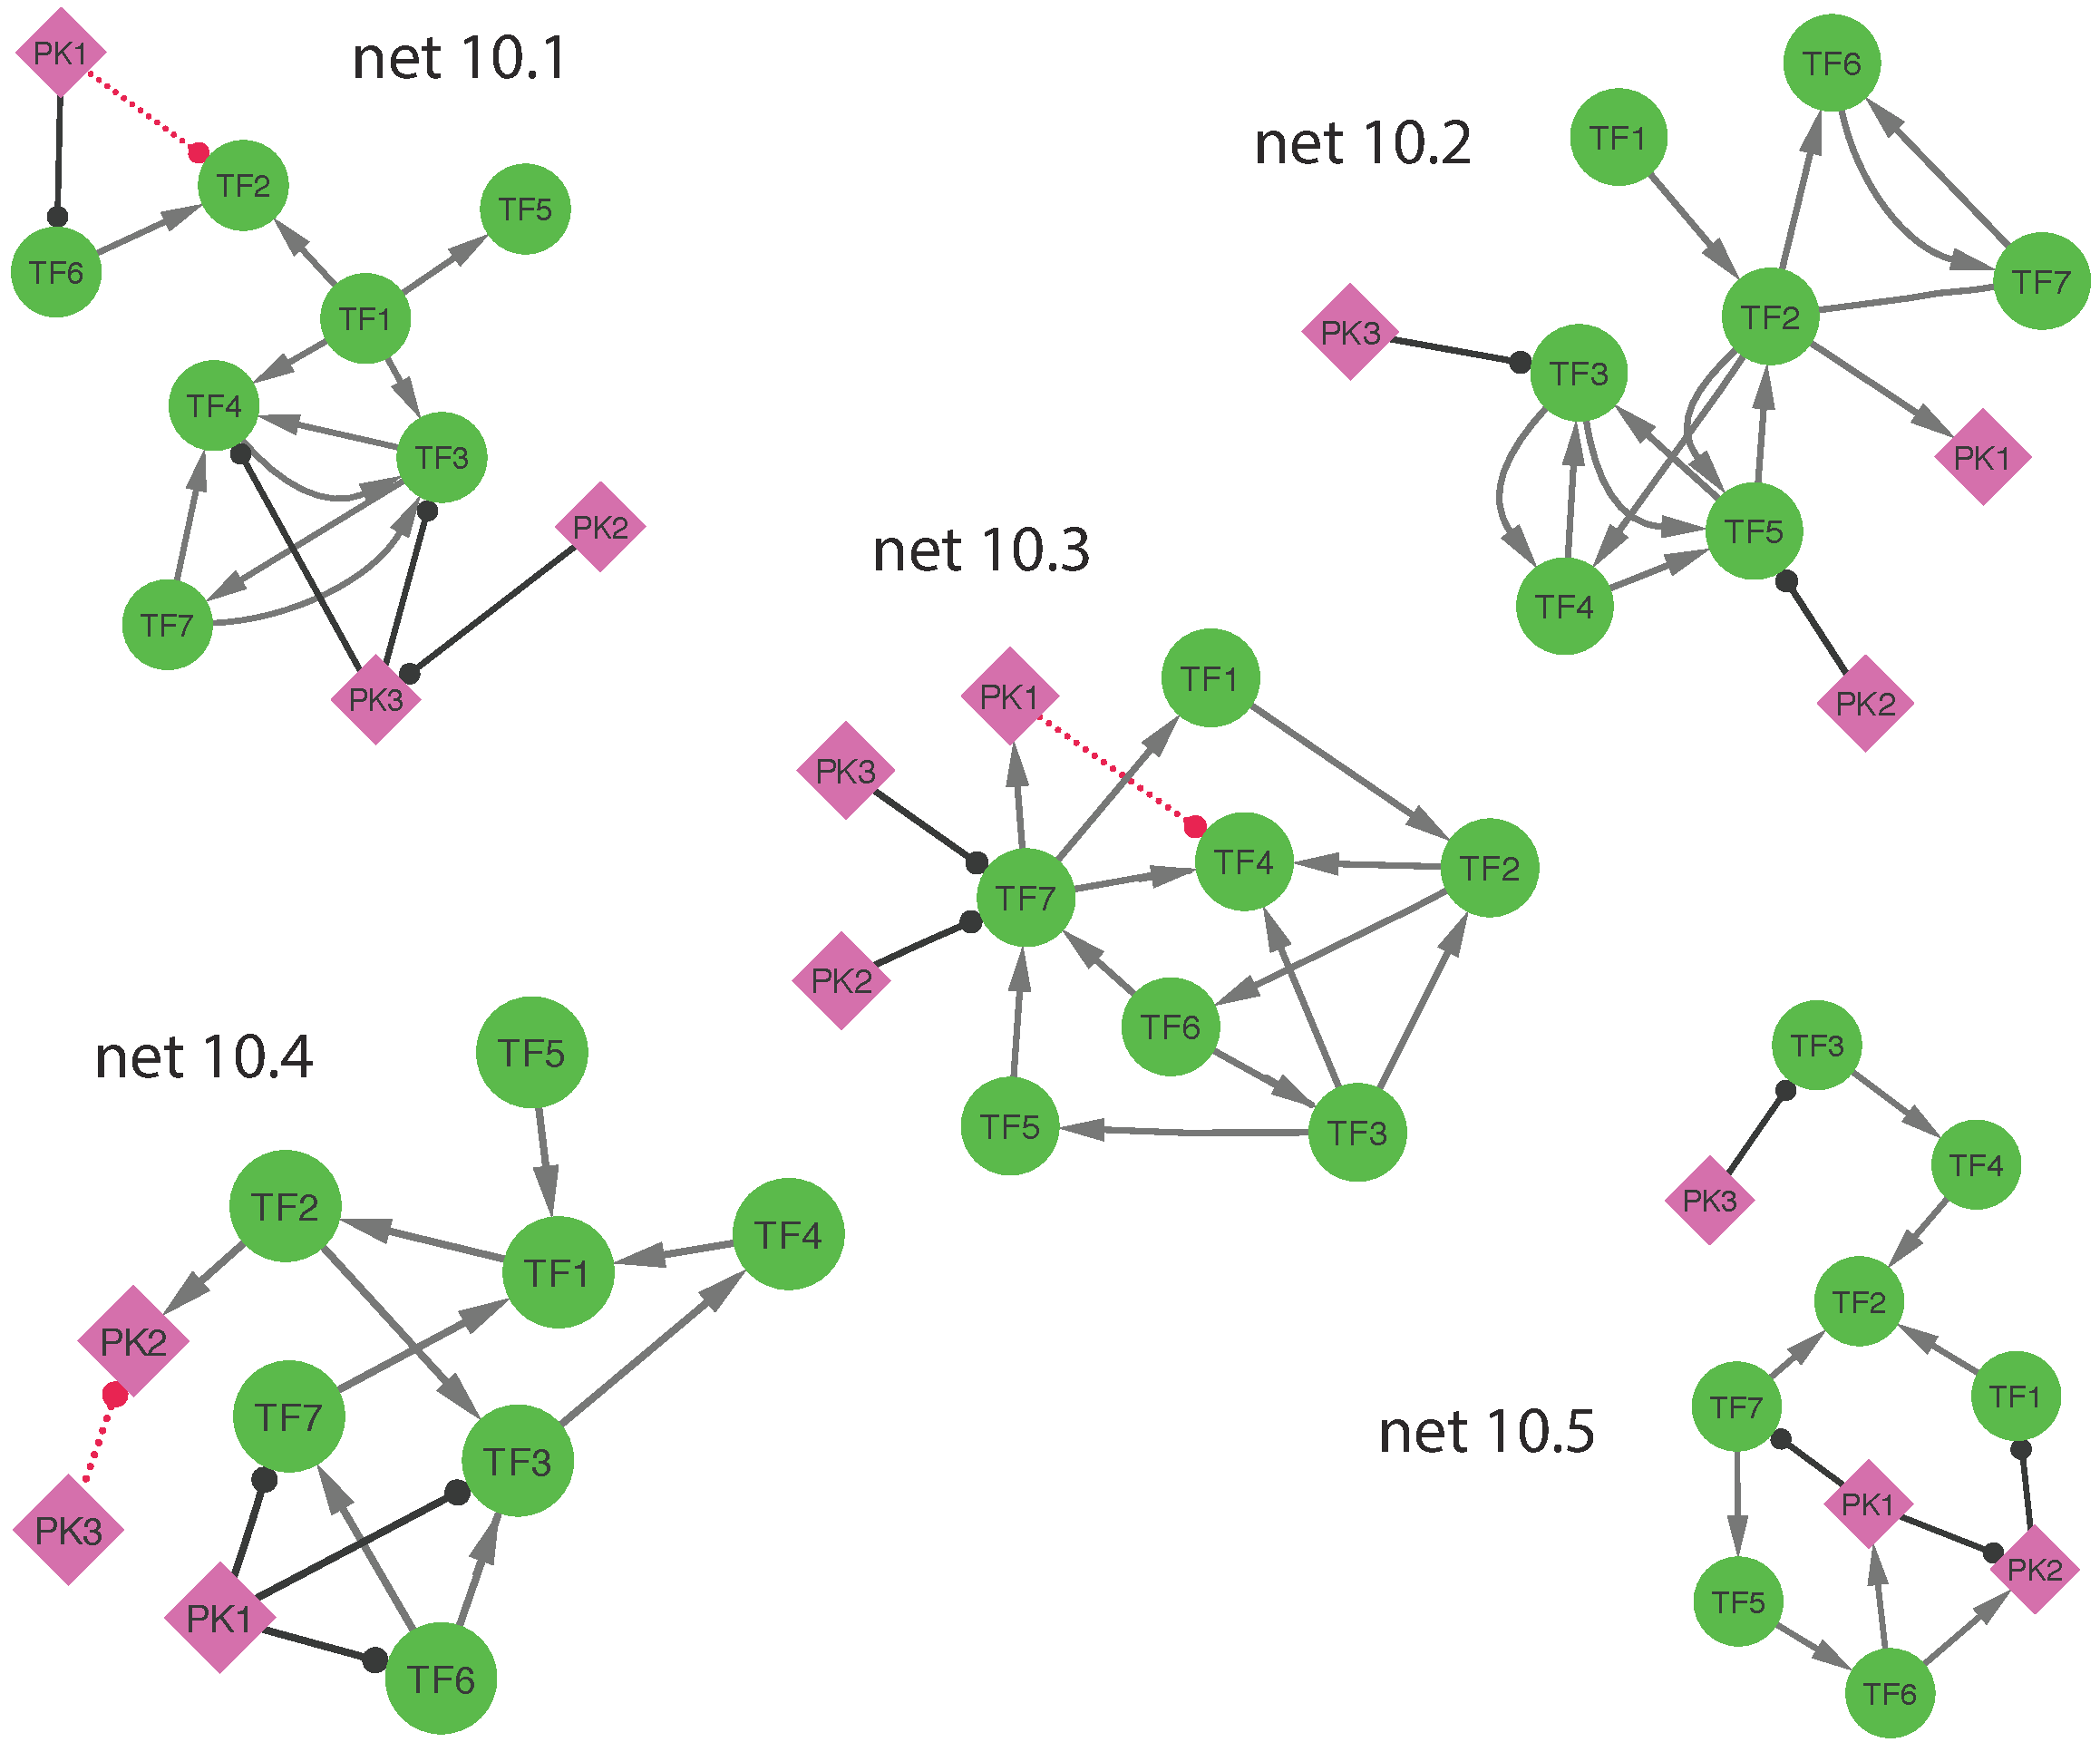
\includegraphics[height=0.85\textheight]{data/fig/nets_10.pdf}
    \caption{\textbf{Networks with 10 nodes.} \textcolor{gray}{Gray} = TF edge, \textcolor{black}{black} = detectable PK edge, \textcolor{red}{red} = silent PK edges. }
    \label{fig:dream4_nets10}
\end{figure}}
{\stepcounter{figure}
\begin{figure}[ht]
    \centering
    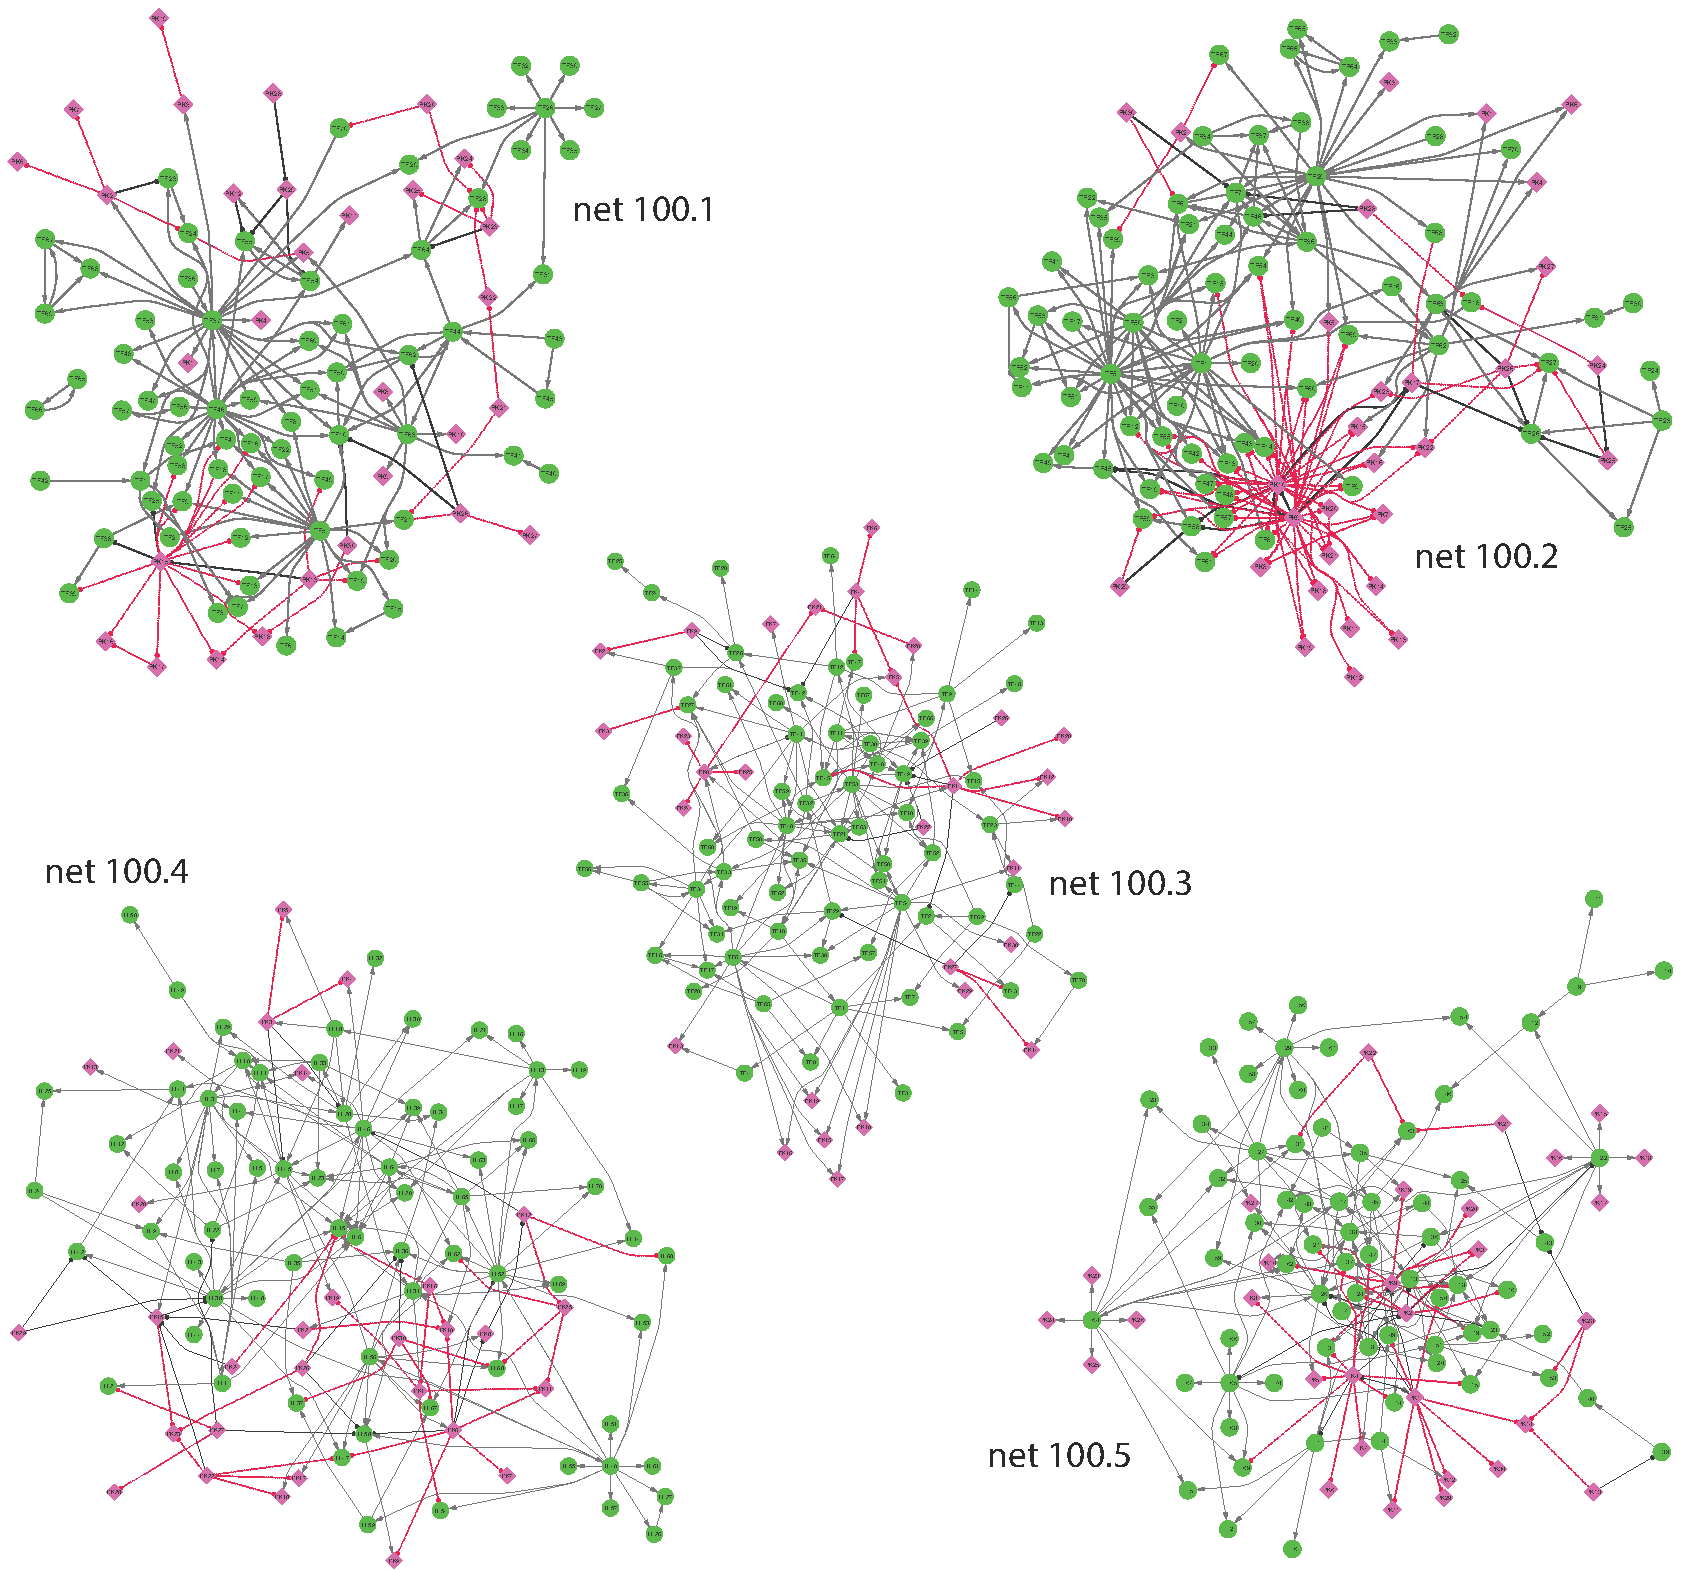
\includegraphics[height=0.85\textheight]{data/fig/nets_100.pdf}
    \caption{\textbf{Networks with 100 nodes.} \textcolor{gray}{Gray} = TF edge, \textcolor{black}{black} = detectable PK edge, \textcolor{red}{red} = silent PK edges. }
    \label{fig:dream4_nets100}
\end{figure}}
% The simulated RNA expression levels are not used since they are simulated using GeneNetWeaver which does not use kinase effects in its gene regulation model. The gold standard true edges are used here. They are given as a list of all pairs of nodes with a 1 or 0 to indicate presence or absence of a directed edge. This was formatted as an adjacency matrix of ones and zeros with edge source nodes as column names and edge target nodes as row names.
% The first~70\% of nodes are used as transcription factors and the remaining~30\% as kinase/phosphatases to roughly match the proportions observed in the yeast data~(\autoref{sec:yeast_data}). So, for 10 node networks there are 7 nodes assigned as TFs and 3 assigned as PKs, for 100 node networks there are 70 assigned as TFs and 30 as PKs.
% The graphs are shown for networks of 10 nodes~(\autoref{fig:dream4_nets10}), for networks of 100 nodes~(\autoref{fig:dream4_nets100}), as well as larger versions of 100 node networks~(\autoref{app:dream_nets}). Each graph are plotted with unsigned edges between TFs and PKs. As discussed in~\autoref{sec:unobservable}, there are certain circumstances where a PK to TF edge will be silent in RNA knockout measurements. These edges are here referred to as undetectable or silent edges.
\end{column}
\end{columns}
\end{frame}

% \begin{frame}{DREAM challenge networks}
% \begin{table}[ht]
% \caption{\textbf{Gold standard networks.} "detectable PK edge" = has effect on gene expression. "detectable PK nodes" = $\ge1$ detectable in- or outgoing edge. "nonsilent PK nodes" = $\ge1$ detectable outgoing edge. }
% \begin{tabularx}{\textwidth}{@{}XXXXXX@{}}
%     \toprule
%     & TF edges & PK edges & \pbox[t]{4cm}{detectable \\ PK edges} & \pbox[t]{4cm}{detectable \\ PK nodes} & \pbox[t]{4cm}{nonsilent \\ PK nodes} \\
%     \midrule
%     net 10.1 & 10 & 5 & 4 & 3 & 3 \\
%     net 10.2 & 14 & 2 & 2 & 3 & 2 \\
%     net 10.3 & 12 & 3 & 3 & 3 & 2 \\
%     net 10.4 & 9 & 4 & 3 & 2 & 1 \\
%     net 10.5 & 8 & 4 & 4 & 3 & 3 \\
%     net 100.1 & 176 & 48 & 13 & 19 & 9 \\
%     net 100.2 & 249 & 101 & 17 & 20 & 9 \\
%     net 100.3 & 195 & 28 & 11 & 23 & 7 \\
%     net 100.4 & 211 & 51 & 19 & 24 & 12 \\
%     net 100.5 & 193 & 52 & 15 & 23 & 7 \\
%     \bottomrule
% \end{tabularx}
% \label{tab:dream_data}
% \end{table}
% % Counts of nodes and edges are summarized in~\autoref{tab:dream_data}. Undetectable edges will not be considered for performance since they will not be detected regardless of inference method. This reduces the effective sizes of the graphs to having the number of PKs listed in column "detectable PK nodes" and to have the PK edges listed in "detectable PK edges".
% % To simulate node values, the gold standard edges are randomly signed and given a random strength. This is generally done by providing a random uniform number in range $[-1,1]$ for each nonzero entry in the gold standard adjacency matrix. It was also tested with standard Gaussian random values.
% % Gene expression levels as log fold-change RNA values are simulated using each of these networks for performance testing of edge inference. Simulation is performed using simple iteration discussed in~\autoref{sec:prim}, or using the GeneNetWeaver extension discussed in~\autoref{sec:gnw_extension}.
% \end{frame}

\subsection{Silent edges}
\begin{frame}{Silent edges}
\label{sec:unobservable}
\begin{columns}
\begin{column}{0.5\textwidth}

\only<1| handout:1>{
Edges silent in RNA logFC data simulated on arbitrary graph

% When inferring a protein-protein or protein-DNA interaction using RNA log fold-change values it is a basic assumption that the RNA values will be affected by the presence or absence of said interaction. In a graph model a TF edge will be observable if the target of the edge is a gene directly measured in the RNA log fold-change data.

% The protein kinases can have outgoing edges with TFs or other PKs as target~(\autoref{fig:unobservable}). If the target of their edge is a TF, then the PK edge will only be detectable if the same can be said for at least one edge from the TF to a measured gene. If the target of the PK edge is another PK, then in order to be detectable, the target will have to have at least one detectable outgoing edge. 


% For real data we will assume that enough genes are recorded that any direct protein-protein or protein-DNA interaction should have some level of effect on gene expression, however small, and that kinase regulation has an effect on gene expression. It is more relevant to consider undetectability for graphs designed artificially from more-or-less random adjacency matrices where it can occur that edges lead to nodes having no outgoing edges themselves.

% A nonsilent node is a node with at least one nonsilent outgoing edge. From a graph with known adjacency matrix $W$ we calculate which nodes are nonsilent with

\begin{equation}
\label{eq:detectable}
\boldsymbol{\omega} =
\sign \sum_{k=0}^K {|W|^\trans}^k
I_T |W|^\trans \boldsymbol{1} 
\end{equation}
\begin{conditions}
|W| & element-wise absolute of $W$ \\
\boldsymbol{1} & vector of 1s
\end{conditions}
% Here $\boldsymbol{\omega}$ is a vector where entry $\omega_i$ will be 1 if node $i$ is detectable and 0 otherwise. The superscript $\trans$ refers to transposing. $W$ has to be square, which it is in all cases where this equation has been applied. $\sign$ is the sign function, $|W|$ is the absolute of $W$, $\boldsymbol{1}$ is a vector of 1s with length $N_T + N_P$. $K$ is the length of the longest cascade of protein kinases, which is found through iterative calculation of $\boldsymbol{\omega}(K)$ as the smallest $K$ for which it holds that $\boldsymbol{\omega}(K) = \boldsymbol{\omega}(K + 1)$.


% \autoref{eq:detectable} can be read as starting with finding all TFs with at least one outgoing edges~($W^\trans \boldsymbol{1} I_T$), and iteratively follow all kinase cascades backwards for each iteration $k$.
}

\only<2| handout:2>{

% The simple network in~\autoref{fig:unobservable} can be used as an example, where we assign some random positive and negative values to each edge. Columns and rows in $W$ are sorted with TF first and PK second, so the order is $\text{TF}_1,\text{TF}_2,\text{TF}_3,\text{PK}_1,\text{PK}_2,\text{PK}_3$.

\begin{subequations}
\begin{align*}
\label{eq:detectable_example}
W &=
\begin{bmatrix} 
0 & 0 & 0 & 0 & 0 & -0.8 \\
0 & 0 & 0 & 0 & 0 & 0.7 \\
0 & 0 & 0 & 0 & -0.1 & 0.3 \\
1.1 & 0 & 0 & 0 & 0 & -0.4 \\
0 & 0 & 0 & 0 & 0 & 0 \\
0 & 0 & 0 & 0 & 0.5 & 0 \\
\end{bmatrix}
\\
|W|^\trans &=
\begin{bmatrix} 
0 & 0 & 0 & 1.1 & 0 & 0 \\
0 & 0 & 0 & 0 & 0 & 0 \\
0 & 0 & 0 & 0 & 0 & 0 \\
0 & 0 & 0 & 0 & 0 & 0 \\
0 & 0 & 0.1 & 0 & 0 & 0.5 \\
0.8 & 0.7 & 0.3 & 0.4 & 0 & 0 \\
\end{bmatrix}
\end{align*}
\end{subequations}

}


\only<3| handout:3>{

\begin{subequations}
\begin{align*}
I_T |W|^\trans \boldsymbol{1}
=
\sum_{k=0}^0 {|W|^\trans}^k
I_T |W|^\trans \boldsymbol{1}
&=
\begin{bmatrix} 
1.1 \\
0 \\
0 \\
0 \\
0 \\
0 \\
\end{bmatrix}
\\
\sum_{k=0}^1 {|W|^\trans}^k
I_T |W|^\trans \boldsymbol{1}
&=
\begin{bmatrix} 
1.1 \\
0 \\
0 \\
0 \\
0 \\
0.88 \\
\end{bmatrix}
\end{align*}
\end{subequations}

}

\only<4| handout:4>{

\begin{subequations}
\begin{align*}
\sum_{k=0}^2 {|W|^\trans}^k
I_T |W|^\trans \boldsymbol{1}
&=
\begin{bmatrix} 
1.1 \\
0 \\
0 \\
0 \\
0.44 \\
0.88 \\
\end{bmatrix}
\\
\sum_{k=0}^3 {|W|^\trans}^k
I_T |W|^\trans \boldsymbol{1}
&=
\begin{bmatrix} 
1.1 \\
0 \\
0 \\
0 \\
0.44 \\
0.88 \\
\end{bmatrix}
\end{align*}
\end{subequations}
}
\only<5| handout:5>{
% There is no change in the calculation from $K=2$ to $K=3$ so we set $K$ equal to 2 and get
\begin{equation*}
\label{eq:silent_example}
\boldsymbol{\omega} = \begin{bmatrix} 
1 \\
0 \\
0 \\
0 \\
1 \\
1 \\
\end{bmatrix}
\quad,\quad
M_s =
\begin{bmatrix} 
1 & 1 & 1 & 1 & 1 & 1 \\
1 & 1 & 1 & 0 & 0 & 0 \\
1 & 1 & 1 & 0 & 0 & 0 \\
1 & 1 & 1 & 0 & 0 & 0 \\
1 & 1 & 1 & 1 & 1 & 1 \\
1 & 1 & 1 & 1 & 1 & 1 \\
\end{bmatrix}
\end{equation*}
% This means that $\text{TF}_2,\text{TF}_3,\text{PK}_1$ are silent nodes. From $\boldsymbol{\omega}$ we can find the set of silent edges, which are all activity regulating edges onto any of the silent nodes. These entries in $W$ of silent edge is shown as zeros in $M_S$~(\autoref{eq:silent_example}), which is the masking matrix that indicates the edges to consider for a performance evaluation on an edge inference attempt. It is clear to spot the four edges in $W$ that are too be ignored if we were to infer edges for this network.
}
\stepcounter{equation}
\end{column}
\begin{column}{0.5\textwidth}
\begin{figure}[ht]
    \centering
    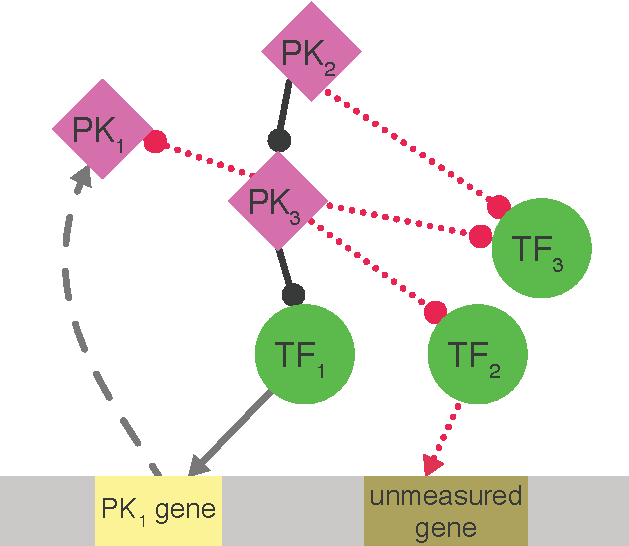
\includegraphics[width=0.6\textwidth]{theory/fig/unobservable.pdf}
    \caption{\textbf{Silent edges.} \textcolor{red}{red} = silent, \textcolor{black}{black} = detectable PK edge, dashed = transcription/translation, \textcolor{darkgray}{dark gray} = TF edge. }
    \label{fig:unobservable}
\end{figure}

\end{column}
\end{columns}
\end{frame}

\begin{frame}{Silent edges - removing $K$}
% As mentioned, $K$ in~\autoref{eq:detectable} is the length of the longest kinase cascade, or more precisely, the iteration where, if we computed further iterations of the sum, it would not change $\boldsymbol{\omega}$. We can simplify by letting $K$ tend to infinity.
for $K\rightarrow\infty$
\begin{equation}
\boldsymbol{\omega} =
\sign \sum_{k=0}^\infty {|W|^\trans}^k
I_T |W|^\trans \boldsymbol{1}
=
\sign \left( \left( \sum_{k=0}^\infty {|W|^\trans}^k \right)
I_T |W|^\trans \boldsymbol{1} \right)
\end{equation}
% If $I-|W|^\trans$ is invertible we can simplify the sum, using the same rule applied by Eberhardt~et~al.~(\autoref{eq:eber_converge.b}). We assume this holds since our system~(\autoref{eq:basic_eberhardt_extension}) is meant to reach equilibrium. It will not be assumed to hold for "gold standard" matrices discussed later~(\autoref{sec:dream_data}), since these does not hold edge values before preprocessing, and would diverge if used as such.
Simplify using same rule applied by Eberhardt~et~al.~(eq.~\ref{eq:eber_converge})
\begin{equation}
\label{eq:detectable_no_K}
\boldsymbol{\omega} =
\sign \left( \left( I - {|W|^\trans} \right)^{-1}
I_T |W|^\trans \boldsymbol{1} \right)
\end{equation}
% \autoref{eq:detectable_no_K} was tested on $W$ given in \autoref{eq:detectable_example}, which as expected produced $\boldsymbol{\omega}$ from \autoref{eq:silent_example} (a tolerance of $>\num{1e-14}$ was used instead of $\sign$ due to the imperfect nature of floating-point computation).
\end{frame}


% \section{Methods}
\section{Inference}
% \begin{frame}{Graphs}
\label{sec:graph}
Signal transduction network
\begin{itemize}
% graph representation
    \item $\mathcal{G} = \left< \mathcal{V}, \mathcal{E} \right>$
% A signal transduction network in a cell can be represented as a graph $\mathcal{G} = \left< \mathcal{V}, \mathcal{E} \right>$, defined as a set of vertices $\mathcal{V}$ and edges $\mathcal{E}$, where each can be assigned attributes, which often are a single scalar. Typically, an edge connects two vertices (nodes) in a graph and can be either undirected or directed, giving it a source and target node. In a hypergraph an edge can connect more than two nodes, which can be useful for metabolic networks where an edge can represent a reaction, for which there can be multiple input and output metabolites represented as the vertices connected to the edge.
% Edges in a graph representing a protein interaction network can represent the physical binding of proteins or binding of proteins to promotors of genes while nodes represent proteins and genes. Edge attributes can represent regulation strength from TFs to genes, while the node attribute can represent gene product concentration. Genes and their protein products can also be represented as a single node. Separate gene and protein representations are useful if it is not assumed to be known which proteins are coded by which genes. When gene and protein product is a single node ambiguity as to whether an edge is regulating the gene~(transcriptional regulation) or the protein~(protein-protein interaction), can be avoided either with an explicit edge attribute signifying its type of interaction, or by basing the type of interaction on the source node of the edge. The latter can be done if a protein is either strictly classified as a transcription regulator or as a protein regulator. Genes and proteins as separate or combined node representations has both been used in this project. A gene and its protein product were separate in~\autoref{sec:convergence_model}, but otherwise considered a single node.
    \item adjacency matrix
% A Graph can be represented as an adjacency matrix where element $i,j$ is the edge from node $j$ to node $i$. The matrix can be symmetrical, which is used to represent an undirected graph where each element represents the connection between two nodes, without influence from choice in $j$ and $i$. Examples of matrices that can be used as a adjacency matrix representation of an undirected graph are covariance, correlation, and partial correlation matrices.

% If the values are restricted to the Boolean case, for instance ones and zeros, it is used for indication of the presence and absence of an edge. Edges with values -1, 0, and 1 can be used to indicate repression, no effect, and activation, respectively. Real value numbers can encode the strength of activation or repression as well. Positive real value numbers can also be used to indicate weighted edges, for instance representing some concept of attraction forces.
\end{itemize}
DAG
\begin{itemize}
    \item paths can be followed to completion
% Directed Acyclic Graphs (DAGs) are a well studied type of graph, used in fields such as machine learning. When a graph is acyclic and directed there exists no path from a node back to itself, that follows the direction of edges. For this reason it is possible to follow any path to completion. Machine learning networks, such as a feedforward network, will be DAGs with a natural progression layer by layer without infinite loops occurring. This makes it possible to define gradients fully describing how each parameter of a model has influence on the value of network outputs in the last layer of the network.
    \item gene regulation is cyclic
% A biological network modelling transcription and translation relies heavily on feedback loops through the transcription and translation of proteins that regulate other iterations of transcription and translation themselves.
% The cycles complicates many aspects of studying the graph, such as describing conditional independence among the nodes~\cite{Tillman2014}.
\end{itemize}
Network inference
% node inference
% Inferring attributes for the vertices of a biological network can be difficult since attributes such as protein or mRNA concentration generally vary a lot depending on cell cycle and environmental factors. Vertex attributes of interest can be the production level or potential production level of a compound for which we are trying to optimize production.
% edge inference
% Inferring the edges of a biological network is an attempt to understand which protein-protein and protein-DNA interactions are taking place, which should be more static than vertex attributes and is what is usually the focus of biological network inference.
% Wanting to find the edges in the network is to say that we are interested in causal connections. As opposed to typical machine learning training of prediction networks we are not interested in finding a nonlinear function mapping from an input to an output as well as possible with a black-box method, but instead to use biological data to shape the causal edges in a network. Predictive performance can however be a secondary objective.
\begin{itemize}
    \item Likelihood based
% Graph learning has been explored using methods maximizing likelihood. Functions are described for the probability of a set of graph edges given observed attributes of the network, and the optimal graph is selected. There are many benefits to a likelihood based approach to edge inference, where the model will describe the basis for inferences and the confidence in them, compared to for instance a "black box" machine learning approach.
% There are also issues with the complexity of likelihood approaches, where graphs with different edges can have equal likelihood of fitting a given dataset, edges might not indicate causality, the amount of data required for a convergent solution grows exponentially with the number of parameters to infer, and heuristics are usually applied to find suboptimal solutions as discussed by Yeang~\cite{Yeang2004}. Yeang goes on to describe and test a model for graph inference where edges are inferred to be present or absent, and if present, inferred to have positive or negative effects of target nodes. The edge strength is used as a p-value to evaluate certainty of predictions. The model is based on log likelihood ratios for hypothesis testing on graph parameters. Knockout data are applied, and the model constrained by protein-protein interaction data and protein-DNA interactions.
\cite{Yeang2004}
% We will combine similar data here, and also use the absolute sizes of predicted edge weights as a score for our belief in the presence in an edge in the graph.
\end{itemize}
\end{frame}


\subsection{Causality and cyclic graphs}
\begin{frame}{Causality and cyclic graphs}
\label{sec:eberhardt}
\begin{columns}
\begin{column}{0.65\textwidth}
% Causal structure learning, where causal edges are inferred on graphs representing real systems, is often performed on DAGs, as described in a review by Heinze-Deml~et~al.~\cite{CausalLearningReview}. DAGs are too simple to use for biological networks where gene transcription products are taken into account. The only model in the review that is designed for cyclic graphs is BackShift, which is an extension of LLC~(Linear, Latents, Cyclic) described by Eberhardt~et~al.~\cite{EberhardtLLC}. Both methods are designed in pursuit of inferring network edges from node attributes observed under different interventions. The interventions are changes to nodes in the graph, which breaks all ingoing edges. In LLC it is assumed to be known which nodes have been intervened on, which is not assumed with BackShift. For knockout studies we know which nodes (genes) have been knocked out, so LLC is discussed here.
% We first assume a system of node values that are controlled linearly by the values from all parent nodes through discreet time steps~(\autoref{eq:eber_linear}).
Eberhardt et al.~\cite{CausalLearningReview}
\begin{subequations}
\label{eq:eber_linear}
\begin{align}
x_i (t) &=
    \sum_j b_{ij} x_j (t - 1) + e_i
\\
\label{eq:eber_linear.b}
\boldsymbol{x}(t) &=
    B \boldsymbol{x} (t - 1) + \boldsymbol{e}
=
    B \left( B \boldsymbol{x} (t - 2) + \boldsymbol{e} \right) + \boldsymbol{e} = ...
\\
&=
    B^t \boldsymbol{x}(0) + \sum_{i=0}^{t-1} B^i \boldsymbol{e}
\label{eq:eber_time.b}
\\
\lim_{t \rightarrow \infty} B^t &= 0
\quad,\quad
\lim_{t \rightarrow \infty} \sum_{i=0}^{t-1} B^i = \left( I - B \right)^{-1}
\qquad\qquad\qquad\text{\cite{Fisher1970}}
\label{eq:eber_converge}
\end{align}
\end{subequations}
% $e_i$ is added as a term to describe latent variables and noise. Latent variables are any hidden variables in the network not included in $\boldsymbol{x}(t)$.
% We can imagine how this generalizes to any time $t$ relative to the start time $t=0$~(\autoref{eq:eber_time}).
% Having cycles in the model means there can be infinite loops of regulation so to capture all regulation effect for cycles in the model $t$ has to tend to infinity. We first have to assume that $\boldsymbol{x}(t)$ converges for $t\rightarrow \infty$. A realistic system is not expected to diverge. Microorganism have exponential growth hindered only by outside factors that we are not considering in the model, but the growth is exponential due to unhindered cell division, but we assume that there is no exponentially increasing level of synthesis inside the cell, and we only model the workings inside a single cell. There is of course another option which is that $\boldsymbol{x}(t)$ fluctuates or in another way neither converges to an equilibrium nor diverges to infinity. Eberhardt~et~al. also considers this and proofs that the conditions for the model can be extended to accept semi-stable systems.
% Each of the two terms defining $\boldsymbol{x}(t)$~(\autoref{eq:eber_time.b}) are found without restriction on $\boldsymbol{x}(0)$ and $\boldsymbol{e}$ when $t$ tends to infinity~(\autoref{eq:eber_converge}):
% The equations hold when all eigenvalues $\lambda_k$ of $B$ satisfies $|\lambda_k| < 1$~\cite{Fisher1970}. The notation with indication of time is dropped when equilibrium is reached:
Equilibrium
\begin{subequations}
\label{eq:eber_simple}
\begin{align}
\lim_{t \rightarrow \infty} \boldsymbol{x}(t) = \boldsymbol{x} &=
    \left( I - B \right)^{-1} \boldsymbol{e}
\\
\left( I - B \right) \boldsymbol{x} &=
    \boldsymbol{e}
\\
\boldsymbol{x} &=
    B \boldsymbol{x} + \boldsymbol{e}
\end{align}
\end{subequations}
\end{column}
\begin{column}{0.35\textwidth}
\begin{figure}[ht]
    \centering
    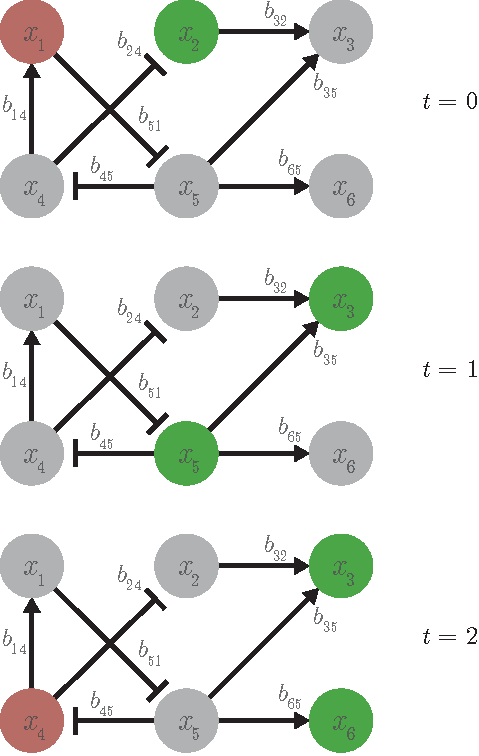
\includegraphics[width=.8\textwidth]{theory/fig/eberhardt.pdf}
    \caption{\textbf{Graph with constant edges.} \\ \textcolor{gray}{Gray} = 0, \textcolor{red!60!black}{red} < 0, \textcolor{green!45!black}{green} > 0.}
    \label{fig:eberhardt}
\end{figure}
\end{column}
\end{columns}
\end{frame}
\begin{frame}{Causality and cyclic graphs - Intervention}
\begin{columns}
\begin{column}{0.65\textwidth}
% We see that the convergence values are defined without referencing the node values at $t=0$ and the expression otherwise exactly matches~\autoref{eq:eber_linear.b}, except that taking a step forward or backward in time does not change the node values anymore.

% The diagonal of $B$ describes edges from nodes onto themselves, self-loops. These are unidentifiable from equilibrium data, since it is impossible to tell the difference between an node with a strong activator and a node with a weaker activator but a strong self-loop only based on steady-state gene expression levels. For this reason the diagonal of $B$ is always set to zeros. 

% The model is then expanded to include a concept of intervention of variables which in the context of biological network experiments is the equivalent of a knockout experiment of one or more genes. The intervention is the replacement of a node with a new value that follows standard Gaussian noise independent of the other variables in the network~(\autoref{eq:eber_intervention}).
Intervention
\begin{subequations}
\label{eq:eber_intervention}
\begin{align}
\boldsymbol{x}_k(t) &=
    U_k B \boldsymbol{x}_k(t-1) + U_k \boldsymbol{e} + \boldsymbol{c}_k
\\
\lim_{t \rightarrow \infty} \boldsymbol{x}_k(t) = \boldsymbol{x}_k &=
    (I - U_k B)^{-1} (U_k \boldsymbol{e} + \boldsymbol{c}_k)
\\
(I - U_k B) \boldsymbol{x}_k &=
    U_k \boldsymbol{e} + \boldsymbol{c}_k
\\
\label{eq:eber_intervention.d}
\boldsymbol{x}_k &=
    U_k B \boldsymbol{x}_k + U_k \boldsymbol{e} + \boldsymbol{c}_k
\end{align}
\end{subequations}
\end{column}
\begin{column}{0.35\textwidth}
\begin{figure}
    \centering
    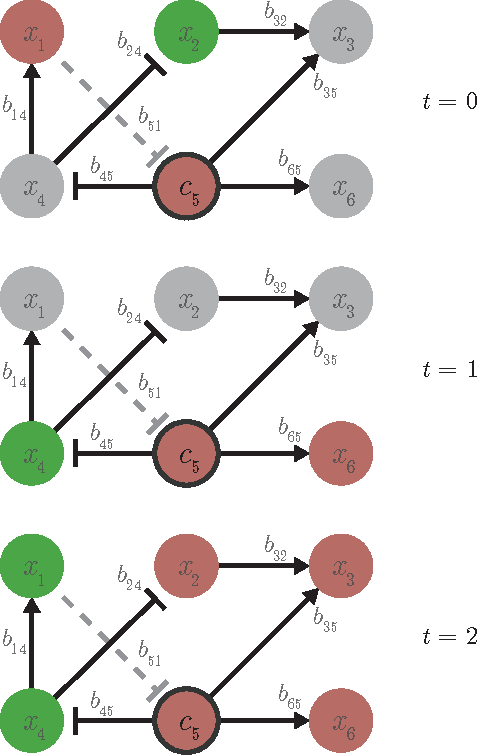
\includegraphics[width=.8\textwidth]{theory/fig/eberhardt_intervention.pdf}
    \caption{\textbf{Intervention on $x_5$.} \\ \textcolor{gray}{Gray} = 0, \textcolor{red!60!black}{red} < 0, \textcolor{green!45!black}{green} > 0.}
    \label{fig:intervention}
\end{figure}
\end{column}
\end{columns}
\end{frame}

\begin{frame}{Causality and cyclic graphs - $E[\boldsymbol{x}_k]$, covariance, and variable separation}
% The noise is given in $\boldsymbol{c}_k$ for the $k$-th experimental setup, where every value is zero except at the indexes of intervened nodes in experimental setup $k$. We refer to $k$ as an experimental setup rather than simply as an experiment to make it clear that the $k$-th experimental setup can be repeated multiple times, creating multiple observations of $\boldsymbol{x}_k$. The effect of other nodes onto the intervened variable is completely removed. 
% This makes sense in terms of a knockout where a removed gene will no longer be regulated by TFs. This is modelled using $U_k$ which is a diagonal matrix of ones, except at the indexes of intervened variables in experiment~$k$, where it has a value of zero. The result is the complete removal of the corresponding rows of $B$ and elements of $\boldsymbol{e}$. 
% A covariance matrix can be estimated if there are multiple observations for each experiment setup~$k$~(\autoref{eq:eber_cov}).
Expectation and covariance
\begin{subequations}
\label{eq:eber_cov}
\begin{align}
E[\boldsymbol{x}_k] &= (I-U_kB) ^{-1} \mu_{\boldsymbol{c}_k}
\\
\Sigma_{\boldsymbol{x}_k}
&=
\E \left[(\boldsymbol{x}_k - \E[\boldsymbol{x}_k] )(\boldsymbol{x}_k - \E[\boldsymbol{x}_k])^\trans \right]
\\
&= (I-U_kB)^{-1} E\left[ (U_k\boldsymbol{e}_k + \boldsymbol{c}_k - \mu_{\boldsymbol{c}_k})(U_k\boldsymbol{e}_k + \boldsymbol{c}_k - \mu_{\boldsymbol{c}_k})^\trans \right] (I-U_kB)^{-\trans}
\\
&= (I-U_kB)^{-1} (\Sigma_{\boldsymbol{c}_k} + U_k\Sigma_{\boldsymbol{e}} U_k) (I-U_kB)^{-\trans}
\end{align}
\end{subequations}
% Where $\mu_{\boldsymbol{c}_k}$ is the expected value of $\boldsymbol{c}_k$, and $\Sigma_{\boldsymbol{x}_k}$ is the covariance matrix of $\boldsymbol{x}_k$. The interesting parts of the covariance matrix are the entries describing covariance between the intervened variables and the passively observed variables. Since it is assumed that no variable has an effect onto intervened variables it can be possible to describe the observed covariance as more than just an undirected covariance edge between the two nodes but instead as a directed edge of causality from the intervened to the non-intervened.
% We denote the elements of vectors and matrices with subscript $\mathcal{J}_k$, $\mathcal{U}_k$, and $\mathcal{V}$ to refer to indexes for nodes intervened on in experimental setup $k$, passively observed in experimental setup $k$ and indexes of all nodes, respectively. We split our expression for $\boldsymbol{x}_k$ from \autoref{eq:eber_intervention.d} into expressions for intervened and non-intervened variables~(\autoref{eq:JU}).
Separating intervened ($\boldsymbol{x}_{\mathcal{J}_k}$) and passively observed ($\boldsymbol{x}_{\mathcal{U}_k}$) variables
\begin{subequations}
\label{eq:JU}
\begin{align}
\boldsymbol{x}_{\mathcal{J}_k} &= \boldsymbol{c}_{\mathcal{J}_k}
\\
\boldsymbol{x}_{\mathcal{U}_k} &= B_{\mathcal{U}_k\mathcal{V}} \boldsymbol{x}_k + \boldsymbol{e}_{\mathcal{U}_k}
\\
&= B_{\mathcal{U}_k\mathcal{U}_k} \boldsymbol{x}_{\mathcal{U}_k} + B_{\mathcal{U}_k\mathcal{J}_k} \boldsymbol{x}_{\mathcal{J}_k} + \boldsymbol{e}_{\mathcal{U}_k}
\\
(I - B_{\mathcal{U}_k\mathcal{U}_k}) \boldsymbol{x}_{\mathcal{U}_k} &=
B_{\mathcal{U}_k\mathcal{J}_k}\boldsymbol{x}_{\mathcal{J}_k} + \boldsymbol{e}_{\mathcal{U}_k}
\\
\boldsymbol{x}_{\mathcal{U}_k} &=
(I - B_{\mathcal{U}_k\mathcal{U}_k})^{-1}(B_{\mathcal{U}_k\mathcal{J}_k}\boldsymbol{x}_{\mathcal{J}_k} + \boldsymbol{e}_{\mathcal{U}_k})
\end{align}
\end{subequations}
\end{frame}

\begin{frame}{Causality and cyclic graphs - Covariance between $\boldsymbol{x}_{\mathcal{J}_k}$ and $\boldsymbol{x}_{\mathcal{U}_k}$}
% The covariance between $\boldsymbol{x}_{\mathcal{J}_k}$ and $\boldsymbol{x}_{\mathcal{U}_k}$ can then be described~(\autoref{eq:causal_cov}).
Covariance between intervened ($\boldsymbol{x}_{\mathcal{J}_k}$) and passively observed ($\boldsymbol{x}_{\mathcal{U}_k}$) variables
\begin{subequations}
\label{eq:causal_cov}
\begin{align}
(\Sigma_{\boldsymbol{x}_k})_{\mathcal{J}_k\mathcal{U}_k} &=
\E \left[ (\boldsymbol{x}_{\mathcal{J}_k} - \E[\boldsymbol{x}_{\mathcal{J}_k}])
(\boldsymbol{x}_{\mathcal{U}_k} - \E[\boldsymbol{x}_{\mathcal{U}_k}])^\trans \right]
\\
&= \E \left[
(\boldsymbol{x}_{\mathcal{J}_k} - \E[\boldsymbol{x}_{\mathcal{J}_k}])
(B_{\mathcal{U}_k\mathcal{J}_k} (\boldsymbol{x}_{\mathcal{J}_k} - \E[\boldsymbol{x}_{\mathcal{J}_k}]))^\trans
\right]
(I - B_{\mathcal{U}_k\mathcal{U}_k})^{-\trans}
\\
&= (\Sigma_{\boldsymbol{c}_k})_{\mathcal{J}_k\mathcal{J}_k} B^\trans_{\mathcal{U}_k\mathcal{J}_k} (I - B_{\mathcal{U}_k\mathcal{U}_k})^{-\trans}
\end{align}
\end{subequations}
% Eberhardt~et~al. deals with what they call canonical experiments to simplify notation where each element in $\boldsymbol{c}_k$ is uncorrelated with zero mean and unit variance. From this and the symmetry of covariance matrices we get expression for covariance between intervened and passively observed that only depend on entries of $B$~(\autoref{eq:eberhardt_cov}). Matrix $T_{\boldsymbol{x}_k}$ is also introduced here.
Using i.i.d. interventions $\boldsymbol{c}_k$
\begin{subequations}
\label{eq:eberhardt_cov}
\begin{align}
(\Sigma_{\boldsymbol{c}_k})_{\mathcal{J}_k\mathcal{J}_k} &= I
\\
(\Sigma_{\boldsymbol{x}_k})_{\mathcal{J}_k\mathcal{U}_k} &= B^\trans_{\mathcal{U}_k\mathcal{J}_k} (I - B_{\mathcal{U}_k\mathcal{U}_k})^{-\trans}
= T_{\boldsymbol{x}_k}^\trans
\\
(\Sigma_{\boldsymbol{x}_k})_{\mathcal{U}_k\mathcal{J}_k} &=
T_{\boldsymbol{x}_k} =
(I - B_{\mathcal{U}_k\mathcal{U}_k})^{-1} 
B_{\mathcal{U}_k\mathcal{J}_k} 
\end{align}
\end{subequations}
\end{frame}

\begin{frame}{Causality and cyclic graphs - Experimental effect}
% A concept of the overall effect from node $x_i$ to $x_u$, referred to as "experimental effect", is introduced~(\autoref{eq:experimental_effect}). It should be read as the total experimental effect from $x_i$ on $x_u$ given the conditions where $\mathcal{J}_k$ refers to the indexes of intervened variables in experimental setup $k$.
Total effect from $x_i$ to $x_u$ is sum of all directed paths
\begin{subequations}
\label{eq:experimental_effect}
\begin{align}
t(x_i \rightsquigarrow x_u || \mathcal{J}_k) &= \sum_{p \in \mathcal{P}(x_i \rightsquigarrow x_u || \mathcal{J}_k)} \prod_{(x_l \rightarrow x_m) \in p} b_{ml}
\\
\label{eq:t_to_b}
&= b_{ui} + \sum_{x_j \in \mathcal{U}_k \setminus \{x_u\}} t(x_i \rightsquigarrow x_j || \mathcal{J}_k) b_{uj}
\end{align}
\end{subequations}

% It is defined as summing the effects from each path from $x_i$ to $x_u$, where the effect along a given path is simply the product over all edge values $b_{ml}$ along that path. Since the graph has cycles there can be an infinite number of paths connecting $x_i$ and $x_u$. 

% In appendix C of 
Eberhardt~et~al.~\cite{EberhardtLLCdetail} proves
\begin{equation}
    t(x_i \rightsquigarrow x_u || \mathcal{J}_k) = (T_{\boldsymbol{x}_k})_{\{x_u\}\{x_i\}}
\end{equation}

%, which means that the experimental effect is equal to the element $u,i$ of the covariance matrix in the case where $x_i$ is intervened upon and $x_u$ is not. The empirical covariance matrix of observed variables can be used as an approximation of the true covariance matrix and thereby used for finding $t(x_i \rightsquigarrow x_u || \mathcal{J}_k)$ for different indexes of $i$ and $u$. As formulated in \autoref{eq:t_to_b} the values of $t(x_i \rightsquigarrow x_u || \mathcal{J}_k)$ are related to the values of $B$ where multiple observations can form a linear system of equations to solve for $B$.
% The resulting LLC algorithm does exactly this.
LLC (Linear, Latent, Cyclic) algorithm overview
\begin{equation}
\Sigma_{\boldsymbol{x}_k}
\rightarrow
T_{\boldsymbol{x}_k}
\rightarrow
t(x_i \rightsquigarrow x_u || \mathcal{J}_k)
\rightarrow
B
\end{equation}
% An issue arises when the covariance matrix cannot be estimated as is the case if there is only a single observation of $\boldsymbol{x}_k$ for each experimental setup $k$. $t(x_i \rightsquigarrow x_u || \mathcal{J}_k)$ is considered a regression coefficient when regressing $x_u$ over the only manipulated variable $x_i$, which means it is calculated as a linear regression coefficient where each observation is treated as the expected value~(\autoref{eq:t_regress}).
If covariance is unknown
\begin{equation}
\label{eq:t_regress}
t(x_i \rightsquigarrow x_u || \{x_i\}) \cdot x_i = x_u
\implies
t(x_i \rightsquigarrow x_u || \{x_i\}) = \frac{x_u}{x_i}
\end{equation}

% LLC is available as \texttt{R}-code, which was used for the $B$-method introduced in~\autoref{sec:equilibrium_inference}.


\end{frame}


\begin{frame}<0>{Inference helped by evolution}
\label{sec:evolution}
% The one you were supposed to have used is "Improving gene network inference by comparing expression time-series across species, developmental stages or tissues" by Guillaume Bourque and David Sankoff from Canada.
Interspecies data
\begin{itemize}
    \item protein interactions
    \item sequence data~\cite{KEGG}
% Interspecies data and other data sources can be included in the effort of protein interaction and gene regulation inference. Protein interaction data from other species can be used on the expectation that if a protein interaction exists in one species, the orthologous proteins are likely to interact in a different species. Genetic and amino acid sequence data can also be exploited by studying the genetic or amino acid similarities to that of another species, and basing expectations of similarity in protein interaction properties on similarity observed in the orthologous proteins' sequences. Gene and amino acid sequences can be obtained from the KEGG GENES database~\cite{KEGG}.
\end{itemize}
Metabolic networks by Kashima~et~al.~\cite{Kashima2009}
\begin{itemize}
    \item Incomplete protein interactions ($\text{A}^{(k)}$)
    \item interspecies protein similarity ($\text{W}^{(k,l)}, k \ne l$)
    \item intraspecies gene expression similarity ($\text{W}^{(k,l)}, k = l$)
\end{itemize}
% Inference of metabolic networks has been studied, where the metabolic networks were treated as a graph for each species~\cite{Kashima2009}. Nodes are enzymes and edges are undirected, representing enzyme reactions in a metabolic pathway.
% Incomplete adjacency matrices $\text{A}^{(k)}$ were obtained for each species $k$, where values indicate presence, absence, or unknown status of enzyme interactions. Sequence similarities for all pairs of proteins were used for calculation of protein similarity scores as symmetrical positive matrices $\text{W}^{(k,l)}$ comparing species $k$ and $l$, where $k\ne l$. Gene expression profiles from DNA microarray hybridization measurements were used for intraspecies similarity matrices $\text{W}^{(k,l)}$, where $k=l$. 
% The idea is to find pairs of orthologous enzymes in different species where their presence or absence of interaction is known for one species but not for the other, and then score the interaction accordingly for the species with incomplete edge information. This is done with $\Tilde{\text{W}}^{(k,l)} = \text{W}^{(k,l)} \otimes \text{W}^{(k,l)}$, where $\otimes$ is the Kronecker product. $\Tilde{\text{W}}^{(k,l)}$ holds the product of each combination of elements of $\text{W}^{(k,l)}$, thereby scoring each enzyme interactions based on how likely it is that the two enzymes involved are orthologous.
% Edge scoring matrices were then inferred by minimizing a loss function that depends on each~$\Tilde{\text{W}}^{(k,l)}$, and~$\text{A}^{(k)}$. Naturally, edges are only inferred for incomplete entries in the adjacency matrices.
% Sequence similarity data could similarly be applied in combination with knockout data for more comprehensive graph inference for signal transduction networks.
\end{frame}

% A few different methods of edge inference on regulatory networks were tested. Most of the code is available at the Bitbucket repository~(\url{https://bitbucket.org/Degnbol/knocknet/}). \texttt{Knocknet} is an interactive command-line environment providing access to most of the functions used in this work, such as basic array operations, simulation of gene regulation and inference of network structures. Some code used is provided in the same repository as independent command-line scripts, such as for plotting and computing which nodes have detectable outgoing edges~(\autoref{sec:unobservable}).

\subsection{Equilibrium model}
\begin{frame}{Equilibrium model}
\label{sec:equilibrium_model}

\begin{columns}
\begin{column}{0.5\textwidth}

LLC works for TF\\
extend to PK with second node attribute

% The LLC model~(\autoref{sec:eberhardt}) attempts to describe causal effects from node value to another through unknown edges. The natural application to gene regulation would be to have each node represent both a gene and its protein product, node values $\boldsymbol{x}$ would represent gene expression levels, and edges would represent protein regulation. The node values can be absolute or relative protein concentrations, in our case log fold-change mRNA measurements~(\autoref{sec:yeast_data}).

% The direct causal effects from one protein to the expression of another makes sense when describing transcription factors that directly regulate gene expression, but is unsuitable when including protein kinases and other protein regulators, since their regulation are on another protein attribute that concentration, for instance the protein's level of phosphorylation. Their influence on the observed gene expression levels is only indirect, which would make them latent variables in LLC, where their effects will have to be described with $\boldsymbol{e}$ as linear effects.
% LLC can be extended to better model indirect regulation effect. Since many proteins can be assumed to be either transcription factors, kinases or phosphatases, it is possible to separate them in the model.

% In order to capture this indirectness, LLC is extended here by adding a second node attribute: "activity". Activity of a protein is meant to describe its state of phosphorylation but since it is unknown if a given protein is in its active form when phosphorylated or dephosphorylated, we generalize the concept of phosphorylation as protein activity.

% A graph in this model is therefore fully defined by a set of edges and nodes, where each edge are directed, so has source and target node attribute, has a signed edge value, and is either categorized as a transcription or activity regulating edge. Each node has three attributes: observed node value indicating relative concentration, unobserved activity attribute, and is category as either TF or PK. The "node value" refers to the observed node value if not explicitly referring to any of the three attributes. We use the simple assumption that a protein cannot be both a transcription regulator and an protein activity regulator, which means that edge types are implicitly known from the type of the edge source.

% The simplest case of regulation between node values is linear effects from node value to node value which can be described as by Eberhardt~et~al. The transcription factors will then have a linear regulation for directly observed node values, while the kinases have linear regulation on the activity attribute of nodes~(\autoref{eq:basic_eberhardt_extension}).


\begin{subequations}
\label{eq:basic_eberhardt_extension}
\begin{align}
x_i(t) &= \sum_{j \in T} w_{ij} a_j(t-1) + e_i^{(x)}
\\
y_i(t) &= \sum_{j \in P} w_{ij} a_j(t-1) + e_i^{(y)}
\\
\boldsymbol{x}(t) &= W I_T \boldsymbol{a}(t-1) + \boldsymbol{e}_x
\\
\boldsymbol{y}(t) &= W I_P \boldsymbol{a}(t-1) + \boldsymbol{e}_y
\end{align}
\end{subequations}
Node attributes:
\begin{conditions}
\boldsymbol{x}(t) & observed in data \\
\boldsymbol{y}(t) & hidden (PK regulated activity) \\
\boldsymbol{a}(t) & effective
\end{conditions}
% Here, $x_i(t)$ is the $i$-th directly observed node value, $y_i(t)$ the activity node attribute, each at discrete timestep $t$. $w_{ij}$ is the edge weight from protein $j$ to $i$, and $a_j(t-1)$ the effective amount of the $j$-th protein at time $t-1$. $e_i^{(x)}$ and $e_i^{(y)}$ are the error terms capturing latent, overlooked variables, and noise. The set $T$ and $P$ are the node indexes for transcription factors and protein kinases, so in matrix/vector notation we can combine all edges in a matrix $W$ where $I_T$ and $I_P$ are diagonal matrices where $I_T$ has 1s in the diagonal corresponding to indexes for TF nodes in $\boldsymbol{x}$, and similarly for $I_P$ in regard to PK node indexes. We sort the proteins with TFs first, followed by PKs~(\autoref{fig:W}).
% The matrix $W$ has zeros in its diagonal for the same reason as why this is enforced for $B$ in LLC~(\autoref{sec:eberhardt}).
\end{column}

\begin{column}{0.5\textwidth}
\begin{figure}[ht]
    \centering
    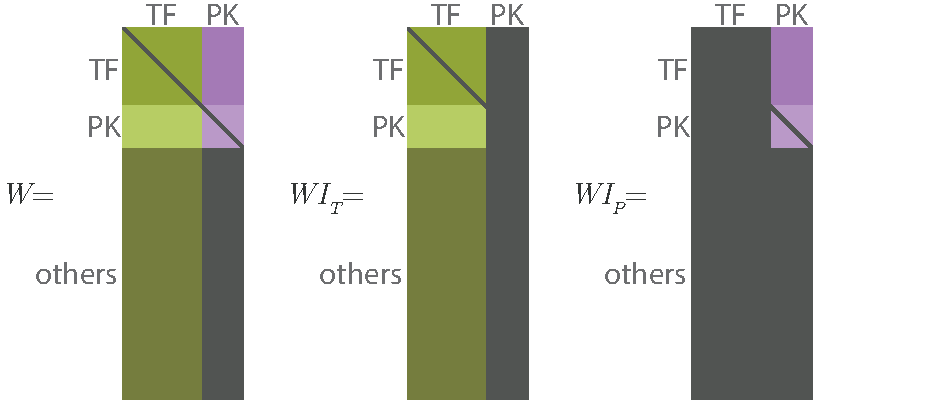
\includegraphics[width=\textwidth]{methods/fig/W.pdf}
    \caption{\textbf{\textit{W}.} Column = edge source, row = target. \\ \textcolor{darkgray}{Dark gray} = 0. Dimensions = $N \times (N_T + N_P)$. }
    \label{fig:W}
\end{figure}
\end{column}
\end{columns}
\end{frame}

\begin{frame}{Equilibrium model}
% Since we are only observing~$\boldsymbol{x}$ we wish to have all other terms for hidden node values disappear which is possible since the model is linear~(\autoref{eq:first_equilibrium_final}).

% If we describe each of the terms as log fold-change versions of absolute measurements for knockout and wildtype experimental conditions, we can get the following~(\autoref{eq:second_equilibrium_def}).
$(t)$ omitted:
\begin{subequations}
\label{eq:second_equilibrium_def}
\begin{equation}
a_i^{(\text{ko})} = y_i^{(\text{ko})} \cdot x_i^{(\text{ko})}
\quad,\quad
a_i^{(\text{wt})} = y_i^{(\text{wt})} \cdot x_i^{(\text{wt})}
\end{equation}\begin{equation}
x_i = \log \frac{x_i^{(\text{ko})}}{x_i^{(\text{wt})}}
\quad,\quad
y_i = \log \frac{y_i^{(\text{ko})}}{y_i^{(\text{wt})}}
\quad,\quad
a_i = \log \frac{a_i^{(\text{ko})}}{a_i^{(\text{wt})}}
= \log \frac{y_i^{(\text{ko})} x_i^{(\text{ko})}}{y_i^{(\text{wt})} x_i^{(\text{wt})}}
= y_i + x_i    
\end{equation}\begin{equation}
\boldsymbol{a}(t) = \boldsymbol{y}(t) + \boldsymbol{x}(t)
\end{equation}
\end{subequations}

% Here $y_i^{(\text{ko})}$ and $y_i^{(\text{wt})}$ are absolute node values, which are typically unmeasured, describing the effective fraction of each protein.

% Owing to the simplicity of a linear model we can cancel out hidden node values as before~(\autoref{eq:second_equilibrium_final}).
Can be shown to converge for $t\rightarrow\infty$
\begin{subequations}
\label{eq:second_equilibrium_final}
\begin{align}
\boldsymbol{a} &= 
    \left(WI_P\boldsymbol{a} + \boldsymbol{e}_y\right) + \boldsymbol{x}
\\
\left(I-WI_P\right) \boldsymbol{a} &=
    \boldsymbol{e}_y + \boldsymbol{x}
\\
\boldsymbol{a} &=
    \left(I-WI_P\right)^{-1} \left(\boldsymbol{e}_y + \boldsymbol{x}\right)
\\
\boldsymbol{x} &=
    WI_T \left(I-WI_P\right)^{-1} \left(\boldsymbol{e}_y + \boldsymbol{x}\right) + \boldsymbol{e}_x
\\
&= WI_T \left(I-WI_P\right)^{-1} \boldsymbol{x} + \boldsymbol{e}
\\
\label{eq:second_equilibrium_final.f}
&= B\boldsymbol{x} + \boldsymbol{e}
\enspace,\enspace B = WI_T \left(I-WI_P\right)^{-1}
\end{align}
\end{subequations}


% Again, the resulting description of observed node values $\boldsymbol{x}$ at equilibrium as a function of itself, can be written as by Eberhardt~et~al. with an extension to $B$. The extension of $B$ is identical to the one at \autoref{eq:first_equilibrium_final.e} with the exception of the 2.
% This model was chosen as the main method going forward based on better intuition in its design, as well as through tests showing little performance difference. 
\end{frame}


\begin{frame}{Equilibrium model - simulation}
\label{sec:prim}

Initial conditions (fig.~\ref{fig:KO_RNA_hist}):
\begin{subequations}
\begin{align}
\boldsymbol{x}_{\mathcal{U}_k} &= 0
\\
\boldsymbol{x}_{\mathcal{J}_k} &\sim \mathcal{N}(\mu=-4, \sigma=1)
\end{align}
\end{subequations}

Simple iteration of eq. \ref{eq:second_equilibrium_final.f} \\
% , where the parameters are chosen based on the observations in . $\boldsymbol{x}(t)$ is then calculated iteratively with \autoref{eq:second_equilibrium_final.f} until approximate convergence is reached, otherwise it will be stopped after 10,000 iterations. Approximate convergence is reached when it holds
Approx. convergence:
\begin{equation}
\label{eq:convergence}
\tfrac{1}{N} \sum_{i=1}^N |x_i(t)-x_i(t-1)| < \epsilon_{tol} \,,\,\epsilon_{tol}=10^{-7}
\end{equation}

\end{frame}

\begin{frame}{Equlibrium model - inference}
\label{sec:equilibrium_inference}

% The obvious way to implement the equations described in \autoref{eq:second_equilibrium_final} in order to infer graph edges will be by applying the algorithm of Eberhardt~et~al., which gives us $B$, and with \autoref{eq:second_equilibrium_final.f} solve for $W$. This cannot be done analytically but is implemented as a gradient descent method where the difference between $B$ and the right hand side of its definition in \autoref{eq:second_equilibrium_final.f} is minimized~(\autoref{eq:loss_B}).
% This approach is referred to as the $B$-method. If there is no covariance matrices for $\boldsymbol{x}_k$ available, $T_{\boldsymbol{x}_k}$ will have to be found using \autoref{eq:t_regress}, which only describes single intervention experiments.

Minimizing a loss function

% Another approach that allows for the inclusion of multiple interventions in an experiment is to minimize~$\boldsymbol{e}$ which is also an attempt at having the least amount of latent variables in the system.
% This approach is referred to as the $\boldsymbol{e}$-minimization method.
% It works by describing the systems of equations from the model in a symbolic math or neural network library in Python. The libraries help by constructing functions for gradients $\dv{\mathcal{L}}{w_{ij}}$, where $\mathcal{L}$ is the loss function and $w_{ij}$ a parameter in $W$. We then minimize the gradient using Adam gradient descent until perceived convergence~\cite{adam}.
% The graph will be sparse which is enforced through L1-regularization. The loss minimized for the $\boldsymbol{e}$-method and $B$-method are:

\begin{subequations}
\label{eq:loss}
\begin{align}
\mathcal{L}_B &=
\sum_{j=1}^N \sum_{i=1}^N
\left(b_{ij} - b_{ij}^{(\text{LLC})}\right)^2
+ \lambda_T \sum_{j \in \text{TF}} \sum_{i=1}^N |w_{ij}| + \lambda_\text{KP} \sum_{j \in \text{KP}} \sum_{i=1}^{N_\text{TF} + N_\text{KP}} |w_{ij}|
\label{eq:loss_B}
\\
\mathcal{L}_{\boldsymbol{e}} &=
\sum_{i=1}^N e_i^2 + \lambda_\text{TF} \sum_{j \in \text{TF}} \sum_{i=1}^N |w_{ij}| + \lambda_\text{KP} \sum_{j \in \text{KP}} \sum_{i=1}^{N_\text{TF} + N_\text{KP}} |w_{ij}|
\label{eq:loss_e}
\end{align}
\end{subequations}

% Here, $\lambda_T$ and $\lambda_P$ are regularization hyperparameters for $W I_T$ and $W I_P$, which means they are chosen to achieve a desired level of sparsity in each of those parts of the weight matrix $W$. They are not necessarily chosen as two different values. $b_{ij}^{(\text{LLC})}$ are values of $B_{\text{LLC}}$ found using LLC. $b_{ij}$ are elements of $B$ which is a function of the trainable parameters in $W$ as described in~\autoref{eq:second_equilibrium_final.f}.


\end{frame}
\subsection{Silent edges}
\begin{frame}{Silent edges}
\label{sec:unobservable}
\begin{columns}
\begin{column}{0.5\textwidth}

\only<1| handout:1>{
Edges silent in RNA logFC data simulated on arbitrary graph

% When inferring a protein-protein or protein-DNA interaction using RNA log fold-change values it is a basic assumption that the RNA values will be affected by the presence or absence of said interaction. In a graph model a TF edge will be observable if the target of the edge is a gene directly measured in the RNA log fold-change data.

% The protein kinases can have outgoing edges with TFs or other PKs as target~(\autoref{fig:unobservable}). If the target of their edge is a TF, then the PK edge will only be detectable if the same can be said for at least one edge from the TF to a measured gene. If the target of the PK edge is another PK, then in order to be detectable, the target will have to have at least one detectable outgoing edge. 


% For real data we will assume that enough genes are recorded that any direct protein-protein or protein-DNA interaction should have some level of effect on gene expression, however small, and that kinase regulation has an effect on gene expression. It is more relevant to consider undetectability for graphs designed artificially from more-or-less random adjacency matrices where it can occur that edges lead to nodes having no outgoing edges themselves.

% A nonsilent node is a node with at least one nonsilent outgoing edge. From a graph with known adjacency matrix $W$ we calculate which nodes are nonsilent with

\begin{equation}
\label{eq:detectable}
\boldsymbol{\omega} =
\sign \sum_{k=0}^K {|W|^\trans}^k
I_T |W|^\trans \boldsymbol{1} 
\end{equation}
\begin{conditions}
|W| & element-wise absolute of $W$ \\
\boldsymbol{1} & vector of 1s
\end{conditions}
% Here $\boldsymbol{\omega}$ is a vector where entry $\omega_i$ will be 1 if node $i$ is detectable and 0 otherwise. The superscript $\trans$ refers to transposing. $W$ has to be square, which it is in all cases where this equation has been applied. $\sign$ is the sign function, $|W|$ is the absolute of $W$, $\boldsymbol{1}$ is a vector of 1s with length $N_T + N_P$. $K$ is the length of the longest cascade of protein kinases, which is found through iterative calculation of $\boldsymbol{\omega}(K)$ as the smallest $K$ for which it holds that $\boldsymbol{\omega}(K) = \boldsymbol{\omega}(K + 1)$.


% \autoref{eq:detectable} can be read as starting with finding all TFs with at least one outgoing edges~($W^\trans \boldsymbol{1} I_T$), and iteratively follow all kinase cascades backwards for each iteration $k$.
}

\only<2| handout:2>{

% The simple network in~\autoref{fig:unobservable} can be used as an example, where we assign some random positive and negative values to each edge. Columns and rows in $W$ are sorted with TF first and PK second, so the order is $\text{TF}_1,\text{TF}_2,\text{TF}_3,\text{PK}_1,\text{PK}_2,\text{PK}_3$.

\begin{subequations}
\begin{align*}
\label{eq:detectable_example}
W &=
\begin{bmatrix} 
0 & 0 & 0 & 0 & 0 & -0.8 \\
0 & 0 & 0 & 0 & 0 & 0.7 \\
0 & 0 & 0 & 0 & -0.1 & 0.3 \\
1.1 & 0 & 0 & 0 & 0 & -0.4 \\
0 & 0 & 0 & 0 & 0 & 0 \\
0 & 0 & 0 & 0 & 0.5 & 0 \\
\end{bmatrix}
\\
|W|^\trans &=
\begin{bmatrix} 
0 & 0 & 0 & 1.1 & 0 & 0 \\
0 & 0 & 0 & 0 & 0 & 0 \\
0 & 0 & 0 & 0 & 0 & 0 \\
0 & 0 & 0 & 0 & 0 & 0 \\
0 & 0 & 0.1 & 0 & 0 & 0.5 \\
0.8 & 0.7 & 0.3 & 0.4 & 0 & 0 \\
\end{bmatrix}
\end{align*}
\end{subequations}

}


\only<3| handout:3>{

\begin{subequations}
\begin{align*}
I_T |W|^\trans \boldsymbol{1}
=
\sum_{k=0}^0 {|W|^\trans}^k
I_T |W|^\trans \boldsymbol{1}
&=
\begin{bmatrix} 
1.1 \\
0 \\
0 \\
0 \\
0 \\
0 \\
\end{bmatrix}
\\
\sum_{k=0}^1 {|W|^\trans}^k
I_T |W|^\trans \boldsymbol{1}
&=
\begin{bmatrix} 
1.1 \\
0 \\
0 \\
0 \\
0 \\
0.88 \\
\end{bmatrix}
\end{align*}
\end{subequations}

}

\only<4| handout:4>{

\begin{subequations}
\begin{align*}
\sum_{k=0}^2 {|W|^\trans}^k
I_T |W|^\trans \boldsymbol{1}
&=
\begin{bmatrix} 
1.1 \\
0 \\
0 \\
0 \\
0.44 \\
0.88 \\
\end{bmatrix}
\\
\sum_{k=0}^3 {|W|^\trans}^k
I_T |W|^\trans \boldsymbol{1}
&=
\begin{bmatrix} 
1.1 \\
0 \\
0 \\
0 \\
0.44 \\
0.88 \\
\end{bmatrix}
\end{align*}
\end{subequations}
}
\only<5| handout:5>{
% There is no change in the calculation from $K=2$ to $K=3$ so we set $K$ equal to 2 and get
\begin{equation*}
\label{eq:silent_example}
\boldsymbol{\omega} = \begin{bmatrix} 
1 \\
0 \\
0 \\
0 \\
1 \\
1 \\
\end{bmatrix}
\quad,\quad
M_s =
\begin{bmatrix} 
1 & 1 & 1 & 1 & 1 & 1 \\
1 & 1 & 1 & 0 & 0 & 0 \\
1 & 1 & 1 & 0 & 0 & 0 \\
1 & 1 & 1 & 0 & 0 & 0 \\
1 & 1 & 1 & 1 & 1 & 1 \\
1 & 1 & 1 & 1 & 1 & 1 \\
\end{bmatrix}
\end{equation*}
% This means that $\text{TF}_2,\text{TF}_3,\text{PK}_1$ are silent nodes. From $\boldsymbol{\omega}$ we can find the set of silent edges, which are all activity regulating edges onto any of the silent nodes. These entries in $W$ of silent edge is shown as zeros in $M_S$~(\autoref{eq:silent_example}), which is the masking matrix that indicates the edges to consider for a performance evaluation on an edge inference attempt. It is clear to spot the four edges in $W$ that are too be ignored if we were to infer edges for this network.
}
\stepcounter{equation}
\end{column}
\begin{column}{0.5\textwidth}
\input{methods/silent_fig.tex}
\end{column}
\end{columns}
\end{frame}

\begin{frame}{Silent edges - removing $K$}
% As mentioned, $K$ in~\autoref{eq:detectable} is the length of the longest kinase cascade, or more precisely, the iteration where, if we computed further iterations of the sum, it would not change $\boldsymbol{\omega}$. We can simplify by letting $K$ tend to infinity.
for $K\rightarrow\infty$
\begin{equation}
\boldsymbol{\omega} =
\sign \sum_{k=0}^\infty {|W|^\trans}^k
I_T |W|^\trans \boldsymbol{1}
=
\sign \left( \left( \sum_{k=0}^\infty {|W|^\trans}^k \right)
I_T |W|^\trans \boldsymbol{1} \right)
\end{equation}
% If $I-|W|^\trans$ is invertible we can simplify the sum, using the same rule applied by Eberhardt~et~al.~(\autoref{eq:eber_converge.b}). We assume this holds since our system~(\autoref{eq:basic_eberhardt_extension}) is meant to reach equilibrium. It will not be assumed to hold for "gold standard" matrices discussed later~(\autoref{sec:dream_data}), since these does not hold edge values before preprocessing, and would diverge if used as such.
Simplify using same rule applied by Eberhardt~et~al.~(eq.~\ref{eq:eber_converge})
\begin{equation}
\label{eq:detectable_no_K}
\boldsymbol{\omega} =
\sign \left( \left( I - {|W|^\trans} \right)^{-1}
I_T |W|^\trans \boldsymbol{1} \right)
\end{equation}
% \autoref{eq:detectable_no_K} was tested on $W$ given in \autoref{eq:detectable_example}, which as expected produced $\boldsymbol{\omega}$ from \autoref{eq:silent_example} (a tolerance of $>\num{1e-14}$ was used instead of $\sign$ due to the imperfect nature of floating-point computation).
\end{frame}






% \begin{frame}{Convergence model}
\label{sec:convergence_model}

% A convergence model was tested, where, instead of formulas describing a system at equilibrium, the system's nonlinear dynamics can be formulated and simulated until approximate convergence. It allows the model to have large amounts of nonlinearity but increases calculation costs significantly.

% A machine learning model was formulated to mimic gene regulation~(\autoref{eq:convergence_model}). It was designed for pseudo-simulation of a wildtype expression converging to the observed RNA expression levels for mutants. The equations described here applies iterative calculation of protein kinase activity for signal cascades, where after $k_{\max}$ iterations the protein kinase activities~$\boldsymbol{a}_P(t,k)$ are used for calculations of transcription factor activities~$\boldsymbol{a}_T(t)$, which are used for calculating predicted gene expression levels~$\boldsymbol{x}(t)$. The loss function $\mathcal{L}_C$ is then formulated as the sum of squared errors of the gene expression prediction $\boldsymbol{x}(t=t_{\max})$ and the measured gene expression levels $y$. Lastly, a L1-regularization is applied on the trainable parameters of the model.

\begin{subequations}
\label{eq:convergence_model}
\begin{align}
\boldsymbol{a}_P (t=0,k=0) &= \boldsymbol{c}_P
\quad,\quad
\boldsymbol{x}(t=0) = \boldsymbol{0}
\\
\boldsymbol{a}_P (t>0,k=0) &= \boldsymbol{a}_P (t-1,k=k_{\max})
\\
\boldsymbol{a}_P (t>0,k>0) &=
U_P \tanh \left(W_{PP} \boldsymbol{a}_P(t,k-1) + M_P \boldsymbol{x}(t-1) \right) + \boldsymbol{c}_P
\\
\boldsymbol{a}_T (t) &=
U_T \tanh \left(W_{PT} \boldsymbol{a}_P(t,k=k_{\max}) + M_T \boldsymbol{x}(t-1) \right) + \boldsymbol{c}_T
\\
\boldsymbol{x}(t) &= \tanh(W_{TX} \boldsymbol{a}_T(t))
\\
\mathcal{L}_C &= \left(\boldsymbol{x}(t=t_{\max}) - \boldsymbol{y}\right)^2
+ \lambda \left(\sum_{j=1}^{N_P}\sum_{i=1}^{N_P}|w_{ij}^{(PP)}| + \sum_{j=1}^{N_P}\sum_{i=1}^{N_T}|w_{ij}^{(PT)}| + \sum_{j=1}^{N_T}\sum_{i=1}^{N}|w_{ij}^{(TX)}| \right)
\end{align}
\end{subequations}
\begin{conditions}
t & time step \\
k & PK cascade step \\
\boldsymbol{x}(t), \boldsymbol{y} & predicted and measured gene expression \\
\boldsymbol{a}_P(t,k), \boldsymbol{a}_T(t) & activity relative to WT for PK, and TF \\
U_P, U_T & mask knocked out PK, and TF \\
\boldsymbol{c}_P, \boldsymbol{c}_T & intervention for PK, and TF \\
M_P, M_T & map gene to product \\
W_{PP}, W_{PT}, W_{TX} & trainable weights
\end{conditions}
% Here, $t$, and $k$ refers to discrete timesteps of gene production and iteration of PK cascade, respectively. $\boldsymbol{a}_P(t,k)$, and $\boldsymbol{a}_T(t,k)$ are activities of protein kinases relative to wildtype. $U_P$, and $U_T$ are masking matrices, removing values of knocked out genes, similar to $U_k$ from~\autoref{sec:eberhardt}. $\boldsymbol{c}_P$ and $\boldsymbol{c}_T$ are vectors of zeros except for indices of knockouts where they are arbitrarily set to -1 to indicate fully reduced activity. Since $\tanh$ is used, all values will be in range $[-1,1]$. $M_P$, and $M_T$ are masking arrays with ones mapping gene indices to their respective protein product indices. $W_{PP}$, $W_{PT}$, and $W_{TX}$ are trainable weight parameters for PK$\rightarrow$PK, PK$\rightarrow$TF, and TF$\rightarrow$gene interactions. $N_P$ is the number of PKs, $N_T$ the number TFs, and $N$ the total count of all genes measured, including TFs, and PKs.

% This model has high computational cost, the formulas are not biologically intuitive, and the model can be criticized for the expectation that convergence is assumed to be reached within a small finite number of iterations. It would be possible to design a model where $\boldsymbol{x}$ is not reset for each gradient descent step, and to allow time $t$ to increase through the entirety of training, however this is beyond what has been tested here.

% Convergence models were initially tested, both with SGD~(Stochastic Gradient Descent), Adam gradient descent, an evolutionary algorithm of learning parameters. A concern was whether the training would be too costly to run. It was found that it was not too costly when testing with Theano or PyTorch, but that error convergence was inadequate for the data in~\autoref{sec:yeast_data}, but perfect for small testing datasets. The equilibrium model is simpler and creates better intuition so the convergence model is not documented in~\autoref{sec:analysis}.
\end{frame}






\section{Data}
% The data used for in-silico experiments are relative RNA expression levels describing how transcription levels are affected by different experimental conditions of gene manipulation, such as gene deletions (knockouts). Protein-protein interaction data is also used describing direct protein regulation, as well as protein-DNA interaction describing transcriptional control.

\begin{frame}{RNA expression levels}
\label{sec:yeast_data}
\begin{columns}
\begin{column}{0.3\textwidth}

% RNA expression levels are gathered from TF, kinase and phosphatase mutant experiments. The TF mutant experiment data were collected from Luscombe et al.~\cite{Luscombe2010} which is based on the original experiments by Hu~et~al.~\cite{Hu2007}. Luscombe et al. improved upon the statistical work performed by Hu~et~al. by considering things like multiple testing problems. The kinase and phosphatase mutant experiments are from Holstege~et~al.~\cite{Holstege2010}. The TF mutants are derived from a BY4741 strain and the kinase/phosphatase mutant from a BY4742 strain.
\small
TF: Luscombe~et~al.~\cite{Luscombe2010}, \\ originally Hu~et~al.~\cite{Hu2007} \\
PK: Holstege~et~al.~\cite{Holstege2010} \\
Name conversion: Tiger~et~al.~\cite{Tiger2012}
\normalsize
% The measurements are gathered for cells at mid log-phase mainly on rich media, but some experiments were done with heat-stress and other stresses. Log-phase is the phase in a typical growth curve of a microorganism where the cells are increasing in number exponentially. The measurements are taken at this time in an attempt to have the cells observed under uniform reproducible conditions with expression levels and regulation as constant as possible.
% The RNA concentrations are measured for both wildtype and the strain under the experimental conditions which in this case are different knockout background. For most experiments a single gene is knocked out, but for some kinase and phosphatase experiments multiple genes have been knocked out.
% The measurements provided are log fold-change values, which are log-transformed ratios comparing the RNA concentration in a knockout experiment with the wildtype concentration~(\autoref{eq:logFC}).

\begin{equation}
\label{eq:logFC}
    x_i = \log_2 \left( \frac{x_i^{(\text{ko})}}{x_i^{(\text{wt})}} \right)
\end{equation}
% Here $x_i$ is the provided transformed value. The superscripts $(\text{ko})$ and $(\text{wt})$ indicates RNA measurements for knockout and wildtype experiment, respectively.
% The values are provided in a table for TF knockouts and another for PK knockouts, each having the knocked out gene indicated as column names and the gene for which RNA is measured indicated as row names. The names are given as popular names, as opposed to systematic names~(ORF~names).
% The log fold-change values are distributed around zero as a bell-curve with lighter tails than a normal distribution~(\autoref{fig:RNA_hist}). The means are $\mu_T \approx -0.023$ and $\mu_P \approx 0.0030$, and standard deviations $\sigma_T \approx 0.24$ and $\sigma_P \approx 0.17$ for transcription factor and kinase/phosphatase knockout experiments, respectively. We see that the majority of genes are not affected strongly be any random knockout.
% From Luscombe~et~al. there are 269 experiments each with a single transcription factor knockout. From Holstege~et~al. there are 144 experiments with a single kinase or phosphatase knockout, 16 with double kinase or phosphatase knockout and a single experiment with a triple knockout totaling at 161 experiments. 5 experiments from Luscombe have the same gene knocked out as from Holstege. An overview of counts can be found in~\autoref{tab:process_counts}.
\end{column}

\begin{column}{0.7\textwidth}
\begin{figure}[ht]
  \centering
  \begin{subfigure}[t]{0.49\textwidth}
  \centering
  \caption{}
  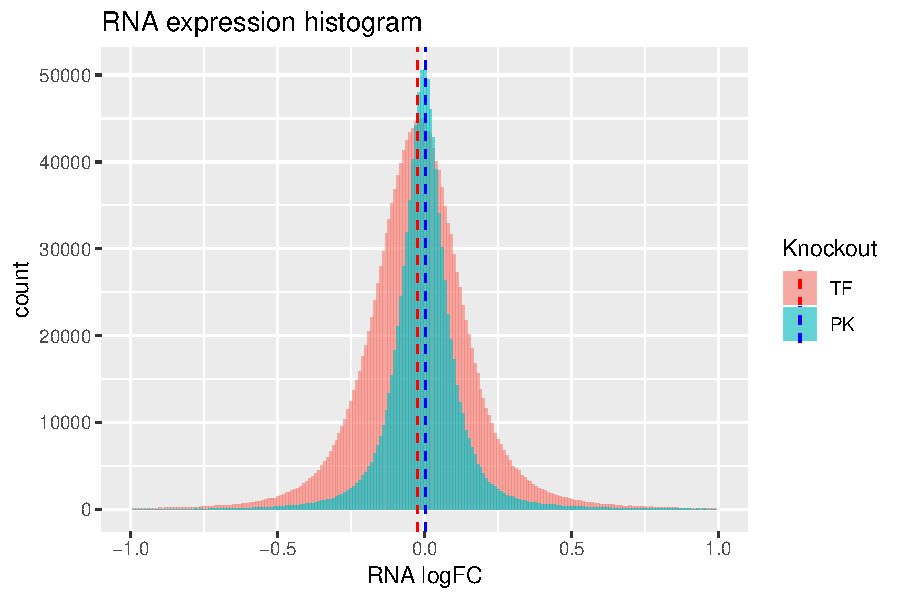
\includegraphics[width=\textwidth]{data/fig/RNA_hist.pdf}
  \label{fig:RNA_hist}
  \end{subfigure}
  \begin{subfigure}[t]{0.49\textwidth}
  \centering
  \caption{}
  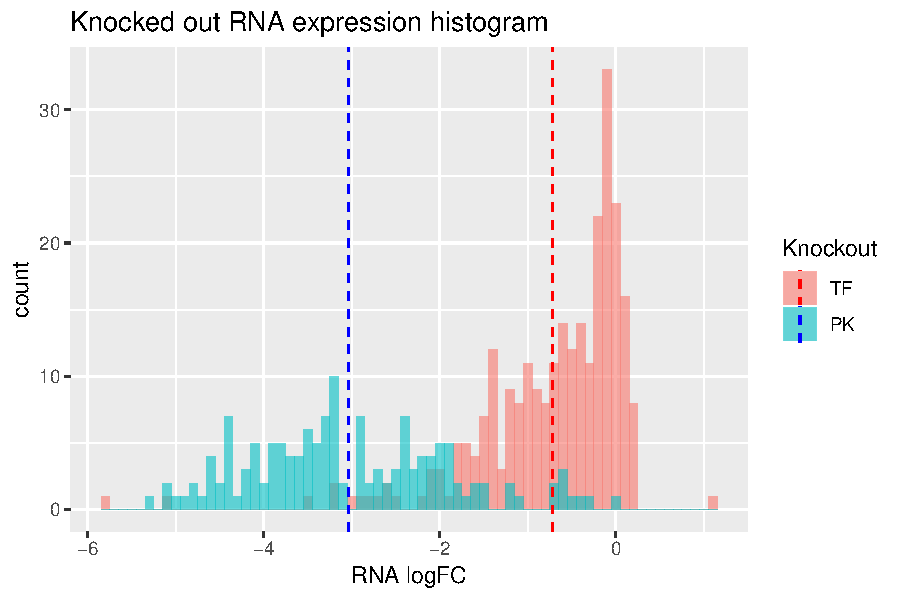
\includegraphics[width=\textwidth]{data/fig/knockout_RNA_hist.pdf}
  \label{fig:KO_RNA_hist}
  \end{subfigure}
  \caption{\textbf{RNA expression level histograms.} all (a) (TF: $269\cdot6253=\num{1.68e6}$, PK: $144\cdot6109=\num{0.88e6}$). Only KOs (b) (TF: 269, PK: 144). Dotted line = mean. }
\end{figure}
% Gene expression levels have been measured for all knockouts~(\autoref{fig:KO_RNA_hist}). The expression levels have mean $\mu_{T,KO} \approx -0.72$ and $\mu_{P,KO} \approx -3.0$ for transcription factor and kinase/phosphatase knockouts, respectively. As these are $\log_2$ fold-change values the means corresponds to a knocked out gene expressed ${\sim}1.6$ and ${\sim}8$ times less than wildtype for TF and PK, respectively.
\end{column}
\end{columns}
% Popular gene names were replaced with systematic names based on a conversion table from Tiger et al.~\cite{Tiger2012}.
% The simplest approach to format the data for use with the model is to filter it to enforce a perfect overlap in the genes for which log-fold change values are measured in the two datasets~(experiments with TF or PK knockouts). This makes it simple to concatenate measurements into a single matrix with known values at all entries.
% 
\small
\begin{table}[ht]
% \caption{\textbf{Protein types counted before and after preprocessing.} Counts of different types of proteins for which gene expression levels were measured. Counts are compared for raw data and data that has been filtered. TF KO, and PK KO refer to the work of Luscombe and Holstege, respectively. "PK and TF" refer to measurements of genes that are the intersection of the TF and PK sets and does therefore not add to the total. "neither" refers to genes that are never knocked out but still observed in the dataset. }
\begin{tabularx}{\textwidth}{@{}XXXXXX@{}}
    \toprule
    & TF & PK & PK and TF & neither & total \\
    \midrule
    TF KO & 269 & 144 & 5 & 5840 & 6253 \\
    PK KO & 266 & 144 & 5 & 5699 & 6109 \\
    processed & 266 & 144 & 5 & 5471 & 5881 \\
    \bottomrule
\end{tabularx}
\label{tab:process_counts}
\end{table}
\normalsize
% The filtering was performed, reducing the number of measured genes as described in \autoref{tab:process_counts}. Any measured gene is categorized as either a transcription factor, kinase/phosphatase, both or neither. We see that three TFs were not measured for kinase/phosphatase knockout experiments, which were removed both in terms of their knockout experiment as well as their expression level in knockout experiments of other transcription factors.

\end{frame}
\begin{frame}{Protein-promoter interactions}
% Data for proteins binding to promoters are gathered from Beyer and Workman et al.~\cite{BeyerWorkman2006}. It is a table of 13,239 transcription factor to gene interactions from 158 transcription factors, where each interaction has an assigned p-value.
Beyer and Workman et al.~\cite{BeyerWorkman2006}: 138 TFs (10,484 edges) \\
Yeastract~\cite{yeastract2017}: 173 TFs (136,813 edges)
\begin{figure}[ht]
  \centering
  \begin{subfigure}[t]{0.38\textwidth}
  \centering
  \caption{}
  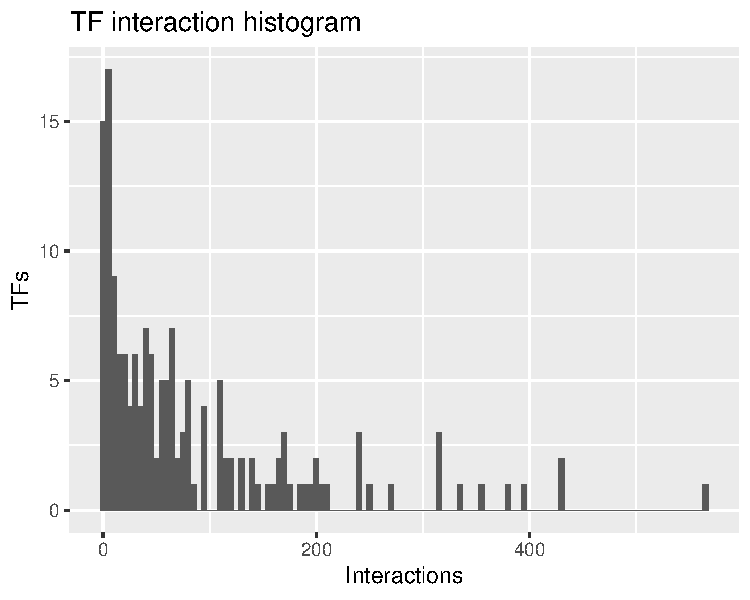
\includegraphics[width=\textwidth]{data/fig/TF_interaction_hist.pdf}
  \label{fig:TF_interactions_hist}
  \end{subfigure}
  \hfill
  \begin{subfigure}[t]{0.5\textwidth}
  \centering
  \caption{}
  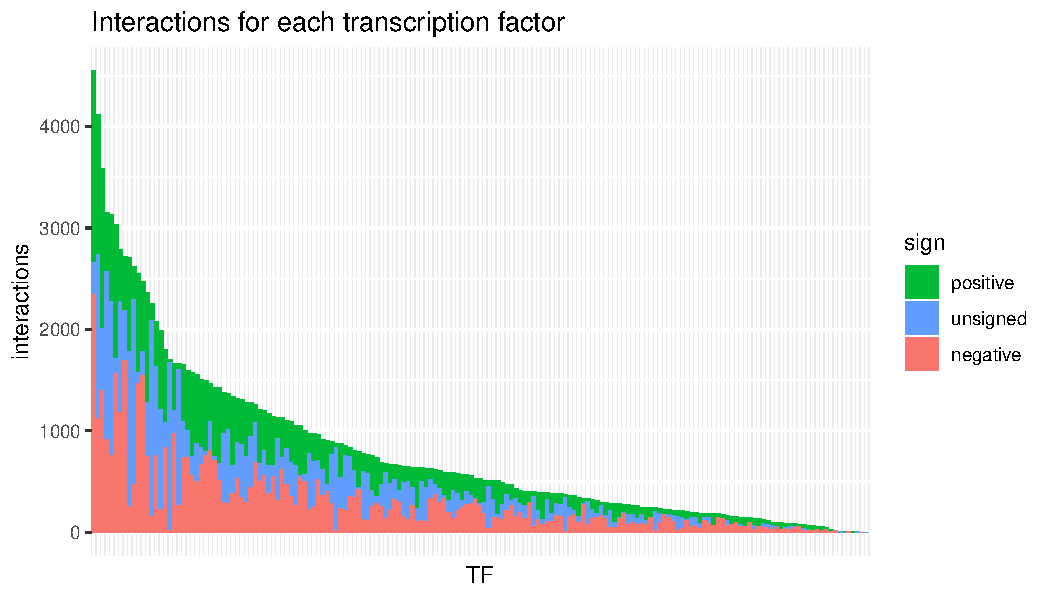
\includegraphics[width=\textwidth]{data/fig/yeastract.pdf}
  \label{fig:yeastract}
  \end{subfigure}
  \caption{\textbf{TF interactions.} TF$\rightarrow$gene interaction histogram for Beyer-Workman (a), and individual TF interactions for Yeastract (b). }
\end{figure}
% Most TFs in the data has in the range of ${\sim}10$ genes they are known to regulate but some regulate in the range of hundreds~(\autoref{fig:TF_interactions_hist}).
% The processed RNA values in \autoref{sec:yeast_data} have 5881 measurements for 266 TF knockout experiments, so not all knocked out TFs have known edges from this protein-promotor dataset. The overlap between the datasets reduces the number of edges from 13,239 to 10,484 with 128 of the 266 TFs having no known regulon. 
% The counts of different types of interactions for each of the 173 TFs are summarized in~\autoref{fig:yeastract}. Most TFs has more than 1 interaction and there is generally both activating and repressing interactions for any given TF. The TF with the most interactions is TF with ORF name YLR131C, which regulates 4550 unique genes in this dataset. 
\end{frame}

% \begin{frame}{Protein-promoter interactions - Yeastract}
% % Another dataset for transcription factors binding to DNA was found from Yeastract~\cite{yeastract2017}. The data was found by using the Yeastract website's function "Generate Regulation Matrix" retrieving all TF interactions documented with either DNA binding or expression evidence. The retrieval was performed separately for TFs acting as activator or inhibitor. The search was performed based on the systematic names of TFs and target genes from the TF dataset described in~\autoref{sec:yeast_data}, which is 266 TFs versus 5881 genes. The resulting tap-separated tables listing all regulatory interactions were used after having all the names converted to systematic names, since they are retrieved as popular names. The conversion was performed using Yeastract's own "ORF List to/from Gene List" conversion utility to ensure that all gene identifiers would be converted sucessfully back to ORF naming.
% % It is assumed that it is not known whether the protein-promotor interaction is positive or negative for TF-gene interactions that were listed in both the activator and repressor sets. They become defined here as unsigned edges, while the remaining activator and repressor interactions become defined as positive and negative edges. The counts of unique transcription factors found and TF-gene interactions are summarized in~\autoref{tab:yeastract}.
% \begin{table}[ht]
% \caption{\textbf{Yeastract TF interactions.} processed = assigning overlap in activators and inhibitors to a third "unsigned" category.}
% \begin{tabularx}{\textwidth}{@{}lYYYcYYYY@{}}
%     \toprule
%      & \multicolumn{3}{c}{raw} & \phantom{aa} & \multicolumn{4}{c}{processed} \\
%     \cmidrule{2-4} \cmidrule{6-9}
%      & activator & inhibitor & all && positive & negative & unsigned & all \\
%     \midrule
%     TFs & 170 & 173 & 173 && 167 & 171 & 157 & 173 \\
%     interactions & 85,098 & 94,286 & 179,384 && 42,527 & 51,715 & 42,571 & 136,813 \\
%     \bottomrule
% \end{tabularx}
% \label{tab:yeastract}
% \end{table}
% % The interactions were from 170 unique TFs in both the activator and repressor lists, as well as 3 additional unique TFs in the repressor list. After assigning the interactions a positive, negative, or unsigned edge, the counts of unique proteins remained about the same, indicating that a transcription factor will usually both have activating and repressing roles. There are $173 \cdot 5881 - 173 = 1,017,240$ possible edges from the TFs described in the Yeastract data to all of the measured genes, excluding self-interactions. About 13\% of possible edges are known~($136,813 / 1,017,240 \approx 0.134$), of which about 69\% have a known sign~($(42,527 + 51,715) / 136,813 \approx 0.689$).
% \end{frame}


% \begin{frame}{Protein-protein interactions}
\begin{columns}
\begin{column}{0.35\textwidth}
% Multiple datasets were found in an effort to have useful prior knowledge about known and probable PK$\rightarrow$PK and PK$\rightarrow$TF edges.

Fiedler~et~al.~\cite{Fiedler2009PK}
\label{sec:fiedler_data}

% Interaction data between proteins are gathered from Fiedler et al.~\cite{Fiedler2009PK}. The protein-protein interactions are from kinases and phosphatases interacting with other kinases, phosphatases and TFs. Fielder et al. collected a table of phosphorylation and dephosphorylation through manual curation of the literature. An Epistatic Miniarray Profile~(E-MAP) of 100,000 genetic interactions were then generated providing scored interactions.



% The scored data includes 537 interactions more for phosphate regulator partners that share a regulated substrate. 304 are pairs where each protein is a kinases or kinase regulator, 65 are pairs where each are phosphatases or phosphatase regulators, and 168 where it is a kinase and a phosphatase, or their regulator, sharing an interaction.

% All scored interactions are used as true interactions which is a total of $166 + 37 + 40 + 9 = 252$ scored interactions and $536 + 113 = 649$ unscored.

% The scored proteins and interactions are not distinct from the unscored ones. There are 63 unique proteins overlapping between scored and unscored datasets, and 206 unique interactions overlapping.


Yeast~KID~\cite{yeastkid}
\label{sec:yeastkid}

% 517 high confidence protein kinase interactions were collected from Yeast KID~\cite{yeastkid}. The table of interactions was found on \url{http://www.moseslab.csb.utoronto.ca/KID/} by searching for all interactions with p-value below 0.05 which is indicated on the page to correspond to a score above 4.52. The table can also be found as supplementary material to the publication which is without p-value cutoff. 74 of the PKs in the Yeast KID dataset overlap with the PKs in the knockout dataset~(\autoref{sec:yeast_data}).


Fasolo~et~al.~\cite{Fasolo2011}
\label{sec:fasolo}

% 1031 directed protein kinase interactions from 84 protein kinases were collected from the work of Fasolo~et~al.~\cite{Fasolo2011}. The proteins were given with popular and standard naming and was converted to systematic names using the conversion table from Tiger~et~al.~\cite{Tiger2012} as well as nomenclature obtained from the Saccharomyces Genome Database~\cite{yeastgenome}.
Name conversion: Tiger~et~al.~\cite{Tiger2012} and Saccharomyces Genome Database~\cite{yeastgenome}

BioGRID~\cite{BioGRID}

% Potential protein kinase interactions were collected from BioGRID~\cite{BioGRID}. Interactions were found from BioGRID's download page for latest release of kinome project interactions (\url{https://downloads.thebiogrid.org/BioGRID/Latest-Release/}). The table has a column describing if the interaction is physical or genetic, which was used to remove genetic interactions. The interactions does not have a described direction so all interactions were copied, reversed, reduced to unique interactions and then filtered so the source of each interaction is a protein kinase. This means that the interactions could be present but that it might be directed incorrectly so the dataset will be used for contrasting the other datasets where edges identified are assumed to be significantly more correct. By only using the 144 protein kinases that are knocked out in~\autoref{sec:yeast_data}, we get 1321 interactions. 
\end{column}

\begin{column}{0.65\textwidth}
\begin{table}[ht]
\caption{\textbf{(Un)scored (de)phosphorylations.} Fiedler et al. "direct" = protein performs (de)phosphorylation, "regulation" = protein regulates (de)phosphorylation through other kinase. Scored and unscored are not distinct. }
\begin{tabularx}{\textwidth}{@{}RYYcYY@{}}
    \toprule
     & \multicolumn{2}{c}{phosphorylation} & \phantom{aa} & \multicolumn{2}{c}{dephosphorylation} \\
    \cmidrule{2-3} \cmidrule{5-6}
     & direct & regulation && direct & regulation \\
    \midrule
    \textit{unscored}\phantom{...........} \\
    proteins & 79 & 34 && 26 & 9 \\
    interactions & 536 & 130 && 113 & 43 \\
    \textit{scored}\phantom{...............} \\
    proteins & 46 & 20 && 17 & 4 \\
    interactions & 166 & 37 && 40 & 9 \\
    \bottomrule
\end{tabularx}
\end{table}
\end{column}
\end{columns}
\end{frame}




\section{Analysis}
\label{sec:analysis}

% Edge inference was performed on a few different graphs where the true gold standard edges are known. Node values are then simulated using these known graphs using two different methods. The node values represent the RNA log fold-change values found experimentally. By inferring the edges using the simulated node values we evaluate the performance of edge inference. Lastly, the experimental yeast data is applied for edge inference for protein kinase interactions, while transcription factor interactions are assumed known.

\begin{frame}{Directed acyclic graph}
\label{sec:dag}
% Inference of edges was first tested as a proof-of-concept on a small DAG~(\autoref{fig:dag}). The DAG is designed with 3 protein kinases and 3 transcription factors, with a combination of positive and negative gene regulation control mediated by the TFs, as well as a combination of positive and negative protein activity regulation mediated by the PKs.
\begin{figure}[ht]
    \centering
    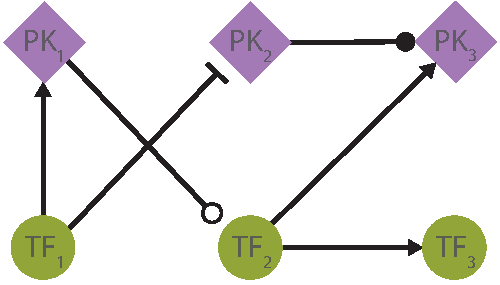
\includegraphics[width=0.3\textwidth]{analysis/fig/dag.pdf}
    \caption{\textbf{DAG example.} Pointed/closed arrowhead: edge value = 1, flat/open: -1. }
    \label{fig:dag}
\end{figure}
% As described in~\autoref{sec:equilibrium_model}, each of the six nodes are defined by observations of their simulated log fold-change RNA values as well as defined by their unobserved activity attribute.
Comparing
\begin{itemize}
    \item simple simulation vs. GNW extension
    \item $\boldsymbol{e}$-minimization vs. LLC
\end{itemize}
\end{frame}

\begin{frame}{Directed acyclic graph - simulation}
\begin{columns}
\begin{column}{0.2\textwidth}
Both simulation methods work intuitively
\end{column}
\begin{column}{0.8\textwidth}
\begin{figure}[ht]
\centering
\begin{subfigure}[b]{0.44\textwidth}\centering\caption{}
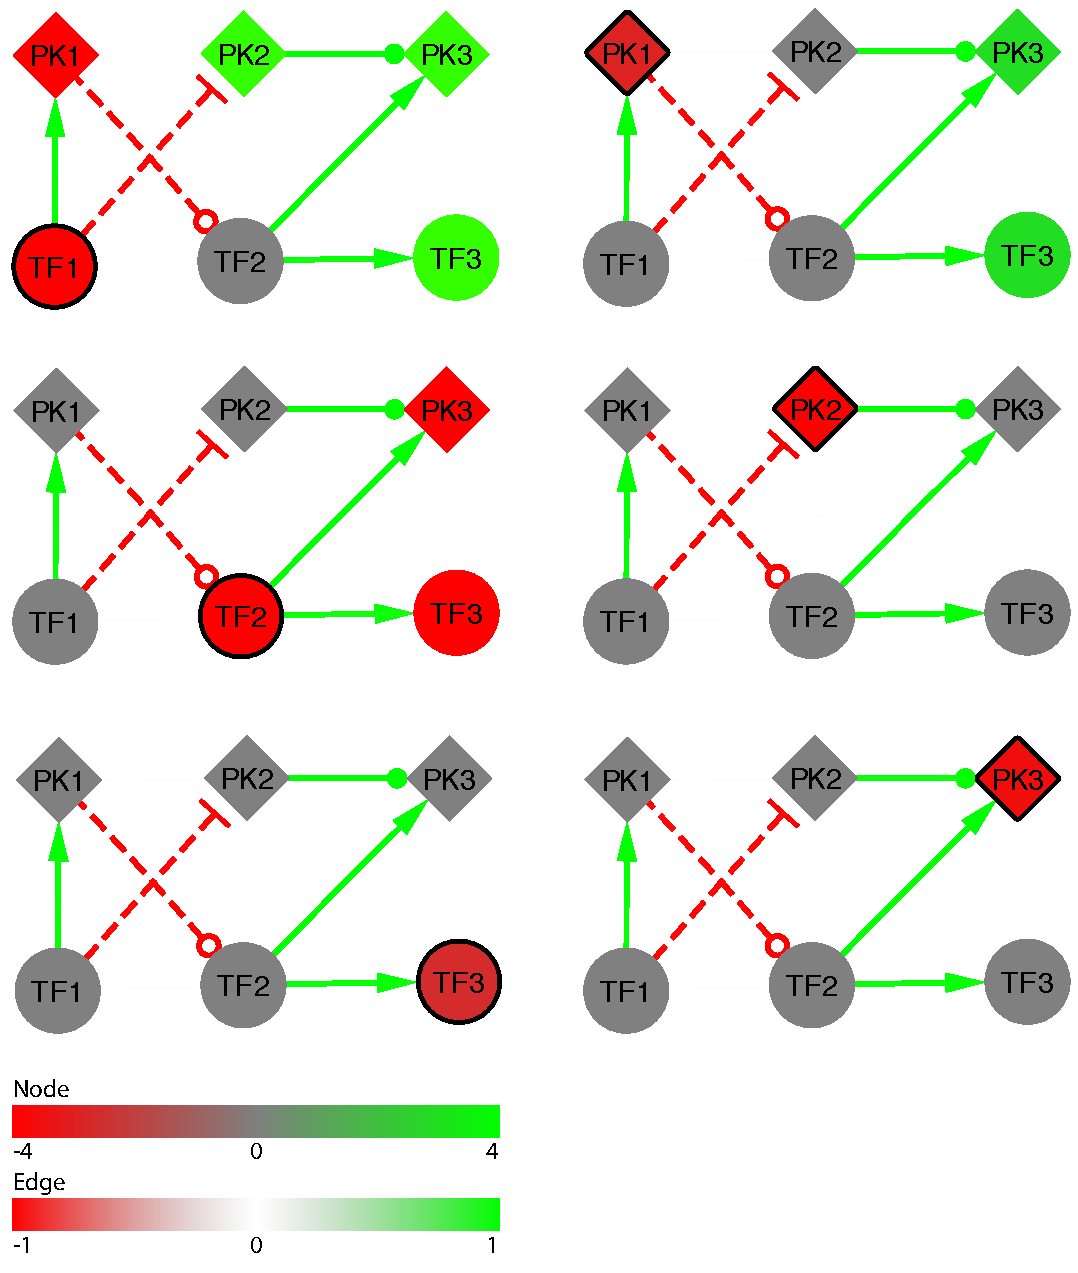
\includegraphics[width=\textwidth]{analysis/fig/prim.pdf}
\end{subfigure}
\hfill
\begin{subfigure}[b]{0.44\textwidth}\centering\caption{}
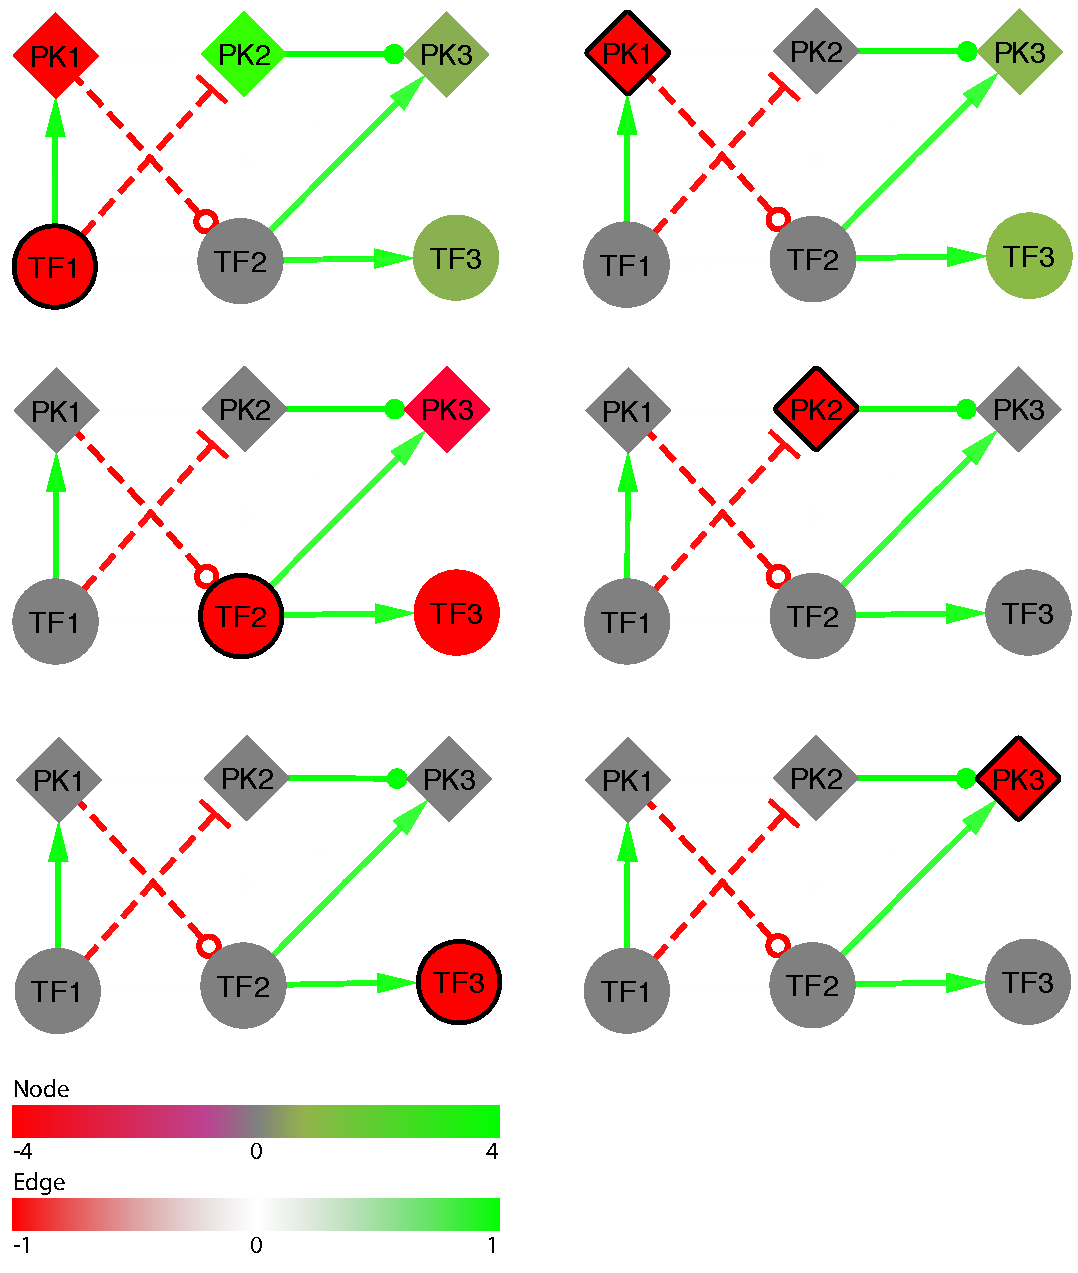
\includegraphics[width=\textwidth]{analysis/fig/gnw.pdf}
\end{subfigure}
\caption{\textbf{DAG node value simulation.} Simple iterative simulation~(a), and extended GeneNetWeaver~(b). LogFC node values. \textcolor{black}{black border} = gene deletion. Edges: true graph. }
\label{fig:dag_data}
\end{figure}

% Two different methods of node value simulation was applied, with the resulting node values indicating with node coloring in~\autoref{fig:dag_data}, where the edges are simply showing the true graph from~\autoref{fig:dag}. The first method is using the inference equations in the simple iterative simulation described in~\autoref{sec:prim}. The second method is applying the GeneNetWeaver kinase extension~(\autoref{sec:gnw_extension}), which is the more realistic simulation approach applying nonlinear gene regulation mechanisms.



% We see how PK regulatory interactions are not directly observed but still detectable through a regulated transcription factor. We also see that the node values are less pronounced when simulated using the GNW extension but otherwise identical in this simple example. Both methods are displaying node values that intuitively would be expected for each given knockout.
\end{column}
\end{columns}
\end{frame}

\begin{frame}{Directed acyclic graph - Inference}

% The $\boldsymbol{e}$-minimization method of edge inference is compared to the original edge inference method LLC~(\autoref{sec:eberhardt}) by using each for edge inference on the simulated node values. The inferred edges on node values simulated using either the simple method or GNW extension are shown in~\autoref{fig:dag_infer}.


\begin{figure}[ht]
\centering
\begin{subfigure}[b]{0.23\textwidth}\centering\caption{}
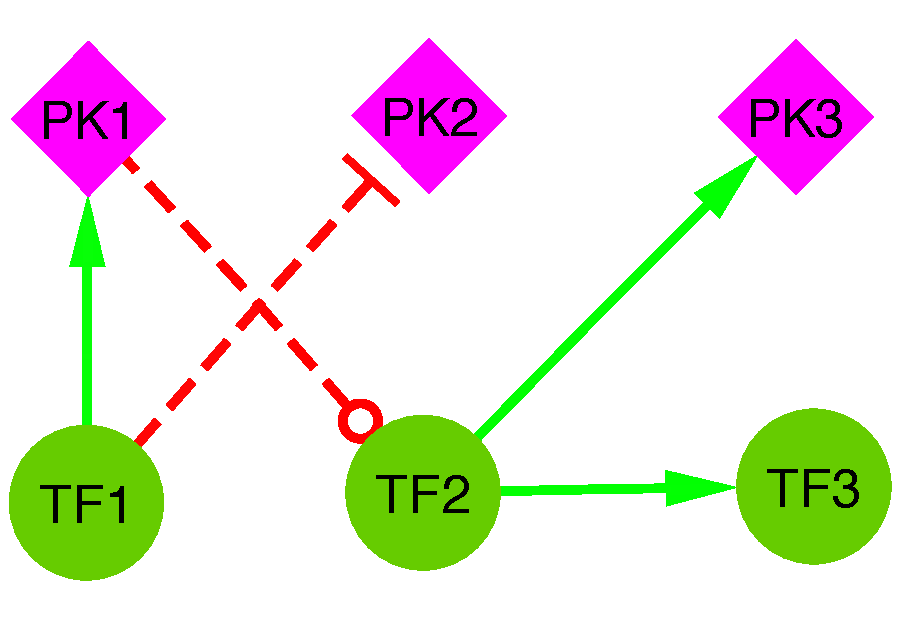
\includegraphics[width=\textwidth]{analysis/fig/weight.pdf}\label{fig:dag_infer.a}
\end{subfigure}
\hfill
\begin{subfigure}[b]{0.23\textwidth}\centering\caption{}
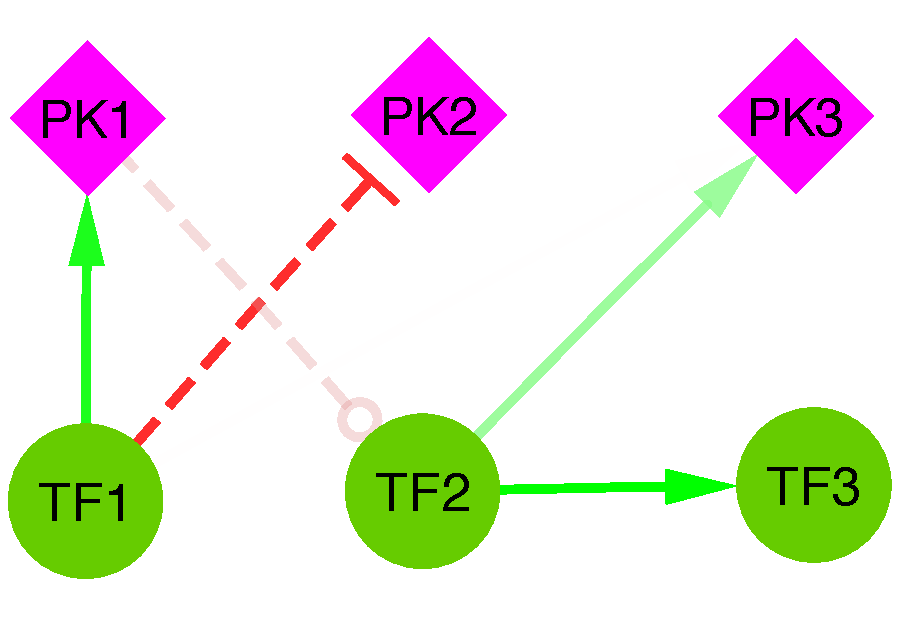
\includegraphics[width=\textwidth]{analysis/fig/gnwweight.pdf}
\end{subfigure}
\hfill
\begin{subfigure}[b]{0.23\textwidth}\centering\caption{}
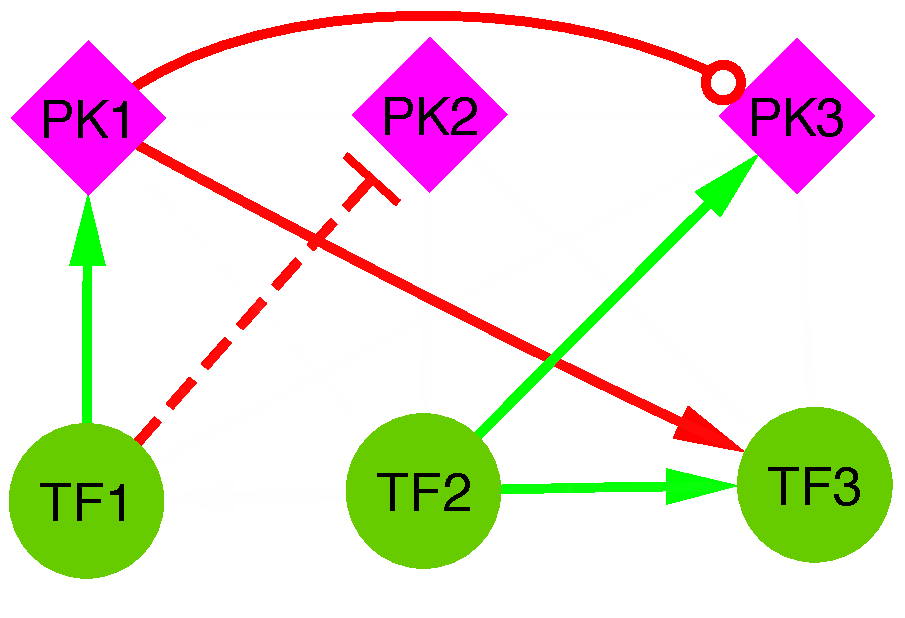
\includegraphics[width=\textwidth]{analysis/fig/B.pdf}\label{fig:dag_infer.c}
\end{subfigure}
\hfill
\begin{subfigure}[b]{0.23\textwidth}\centering\caption{}
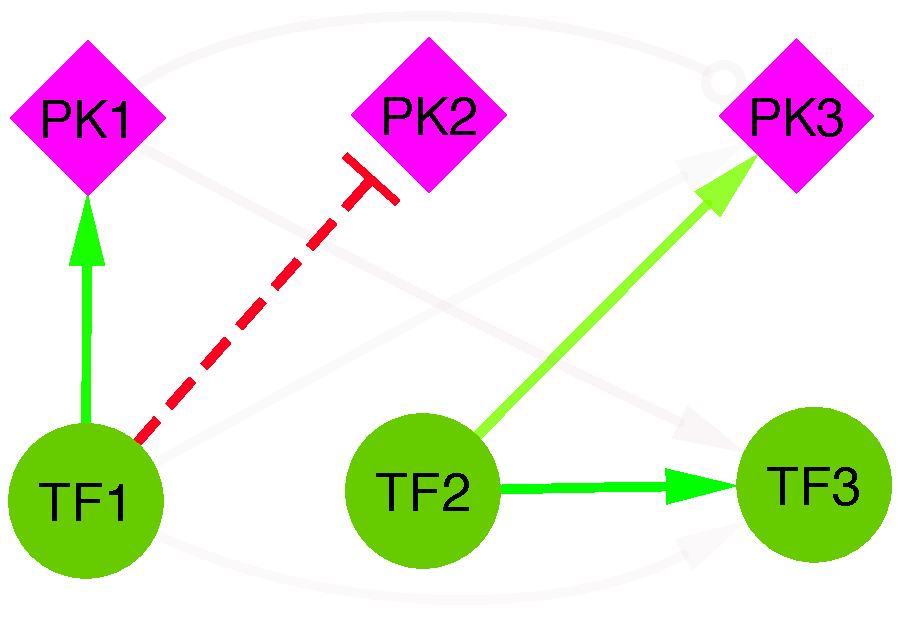
\includegraphics[width=\textwidth]{analysis/fig/gnwB.pdf}
\end{subfigure}
\vskip\baselineskip
\begin{subfigure}[b]{0.25\textwidth}\centering
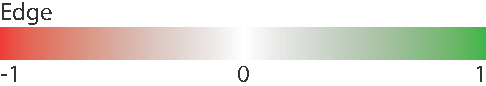
\includegraphics[width=\textwidth]{analysis/fig/edge_legend.pdf}
\end{subfigure}
\caption{\textbf{DAG edge inference.}  $\boldsymbol{e}$-minimization~(a,b), and LLC~(c,d). On simple iterative simulation~(a,c), and GeneNetWeaver kinase extension~(b,d).}
\label{fig:dag_infer}
\end{figure}
$\boldsymbol{e}$-minimization captures indirectness, LLC does not
% We see that LLC correctly predicts the TF edges, which are directly influencing node values, but does not capture any edges from the protein kinases, which are indirectly affecting node values~\autoref{fig:dag_infer.c}. We further see that the $\boldsymbol{e}$-minimization method captures all detectable edges~\autoref{fig:dag_infer.a}. The PK edge from $\text{PK}_2$ to $\text{PK}_3$ is undetectable since $\text{PK}_3$ does not regulate anything. For node values simulated with GNW extension it is the same observations, although some edges appear weaker, which can make them harder to detect in noisy data. However, since edge inference is a boolean classification problem, their weakness is not an issue as long as the edge value is above the threshold used for edge detection.


\end{frame}

\begin{frame}{Cyclic graphs}
\label{sec:toy}
\begin{columns}
\begin{column}{0.4\textwidth}
% We now add cycles to the DAG from before~(\autoref{sec:dag}). The edges are also given randomly selected values in range $[-1,1]$~(\autoref{fig:toy}).
\begin{figure}[ht]
    \centering
    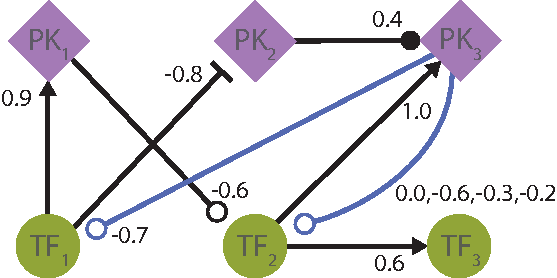
\includegraphics[width=0.7\textwidth]{analysis/fig/toy.pdf}
    \caption{\textbf{Directed cyclic networks.} \textcolor{blue}{blue} = edges added onto DAG. Multiple values: four separate graphs each assigned one of the four values. }
    \label{fig:toy}
\end{figure}
% Four separate graphs are tested to analyse the balance between predicting that an edge is present from a protein kinase to a transcription factor or that the observed effect is mediated through another protein kinase.

\vskip2\baselineskip

$\pk_2\rightarrow\pk_3$ is favored over $\pk_2\rightarrow\tf_{}$ when increasing $\pk_3\rightarrow\tf_{}$
\end{column}

\begin{column}{0.6\textwidth}
\begin{figure}[ht]
\centering
\begin{subfigure}[b]{0.4\textwidth}\centering\caption{}
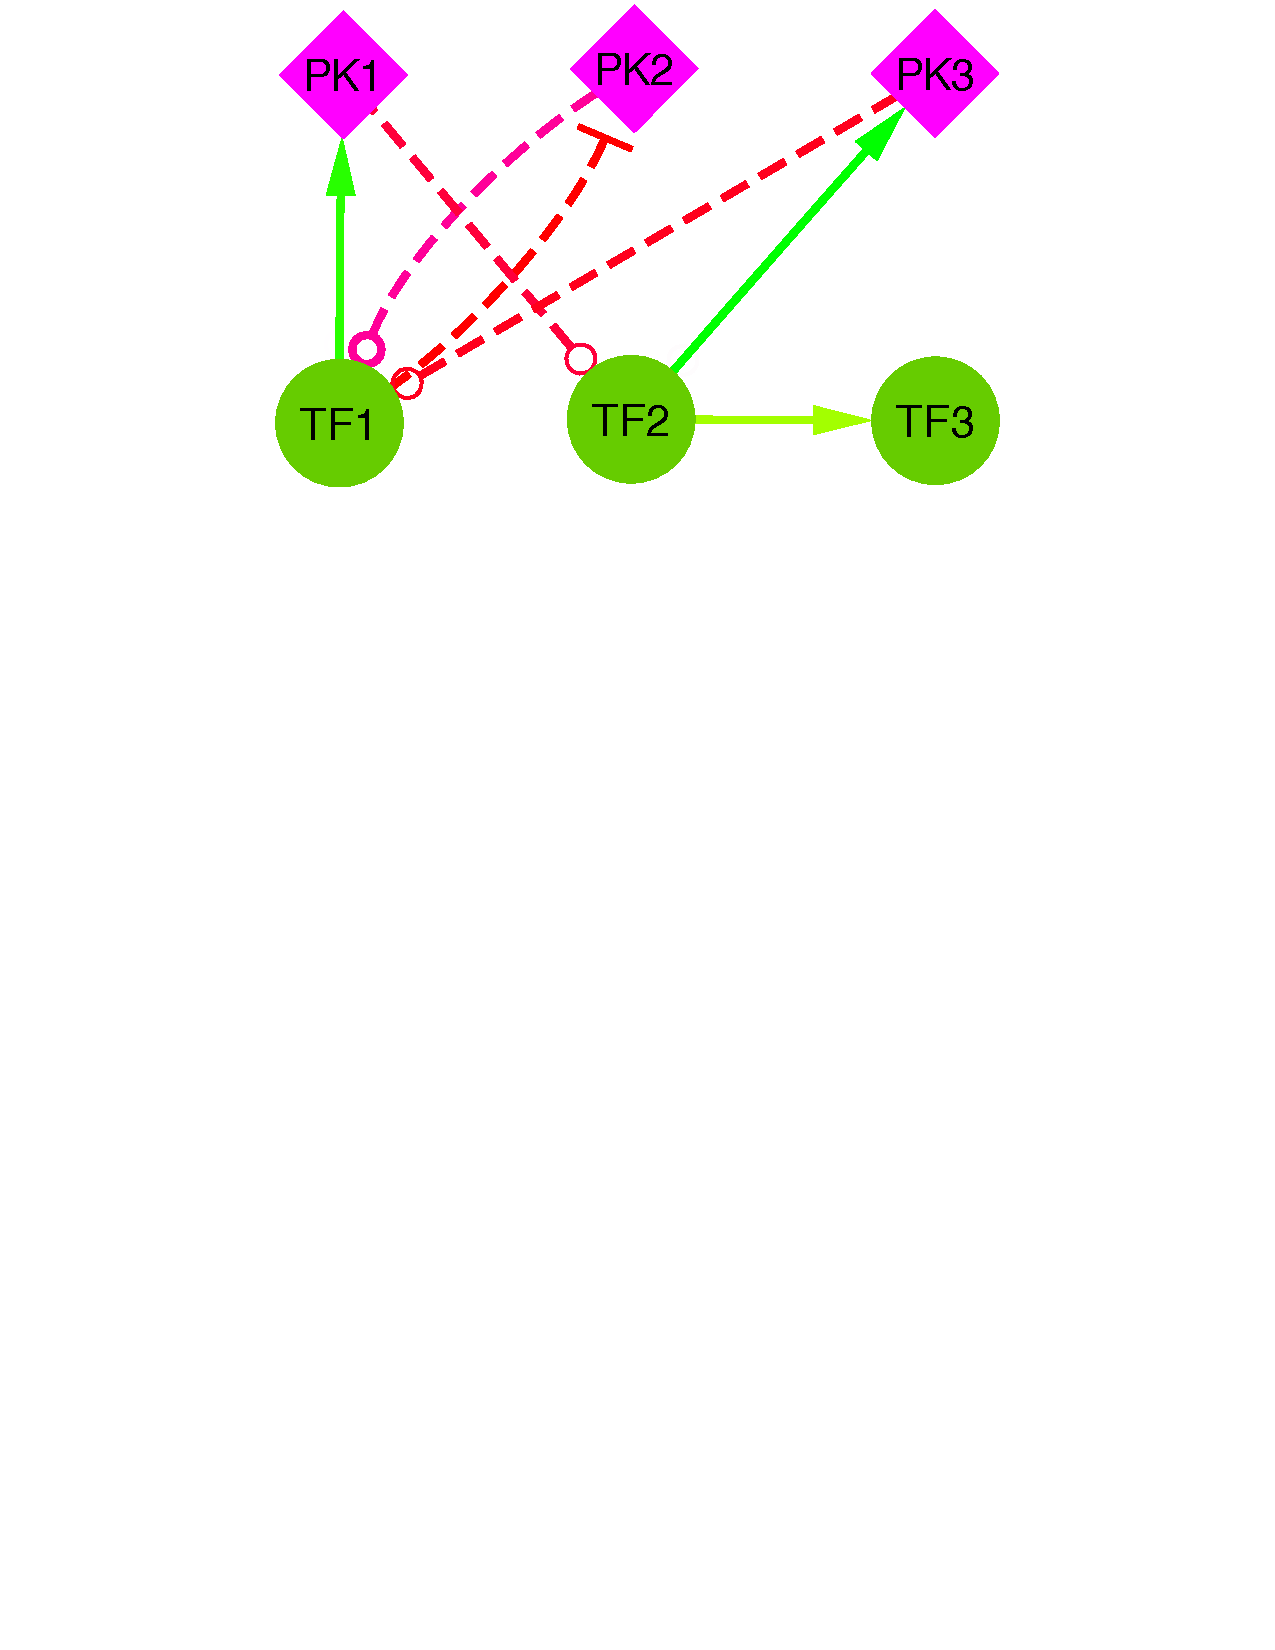
\includegraphics[width=0.8\textwidth]{analysis/fig/cyclic_2.pdf}\label{fig:toy_infer.a}
\end{subfigure}
\quad
\begin{subfigure}[b]{0.4\textwidth}\centering\caption{}
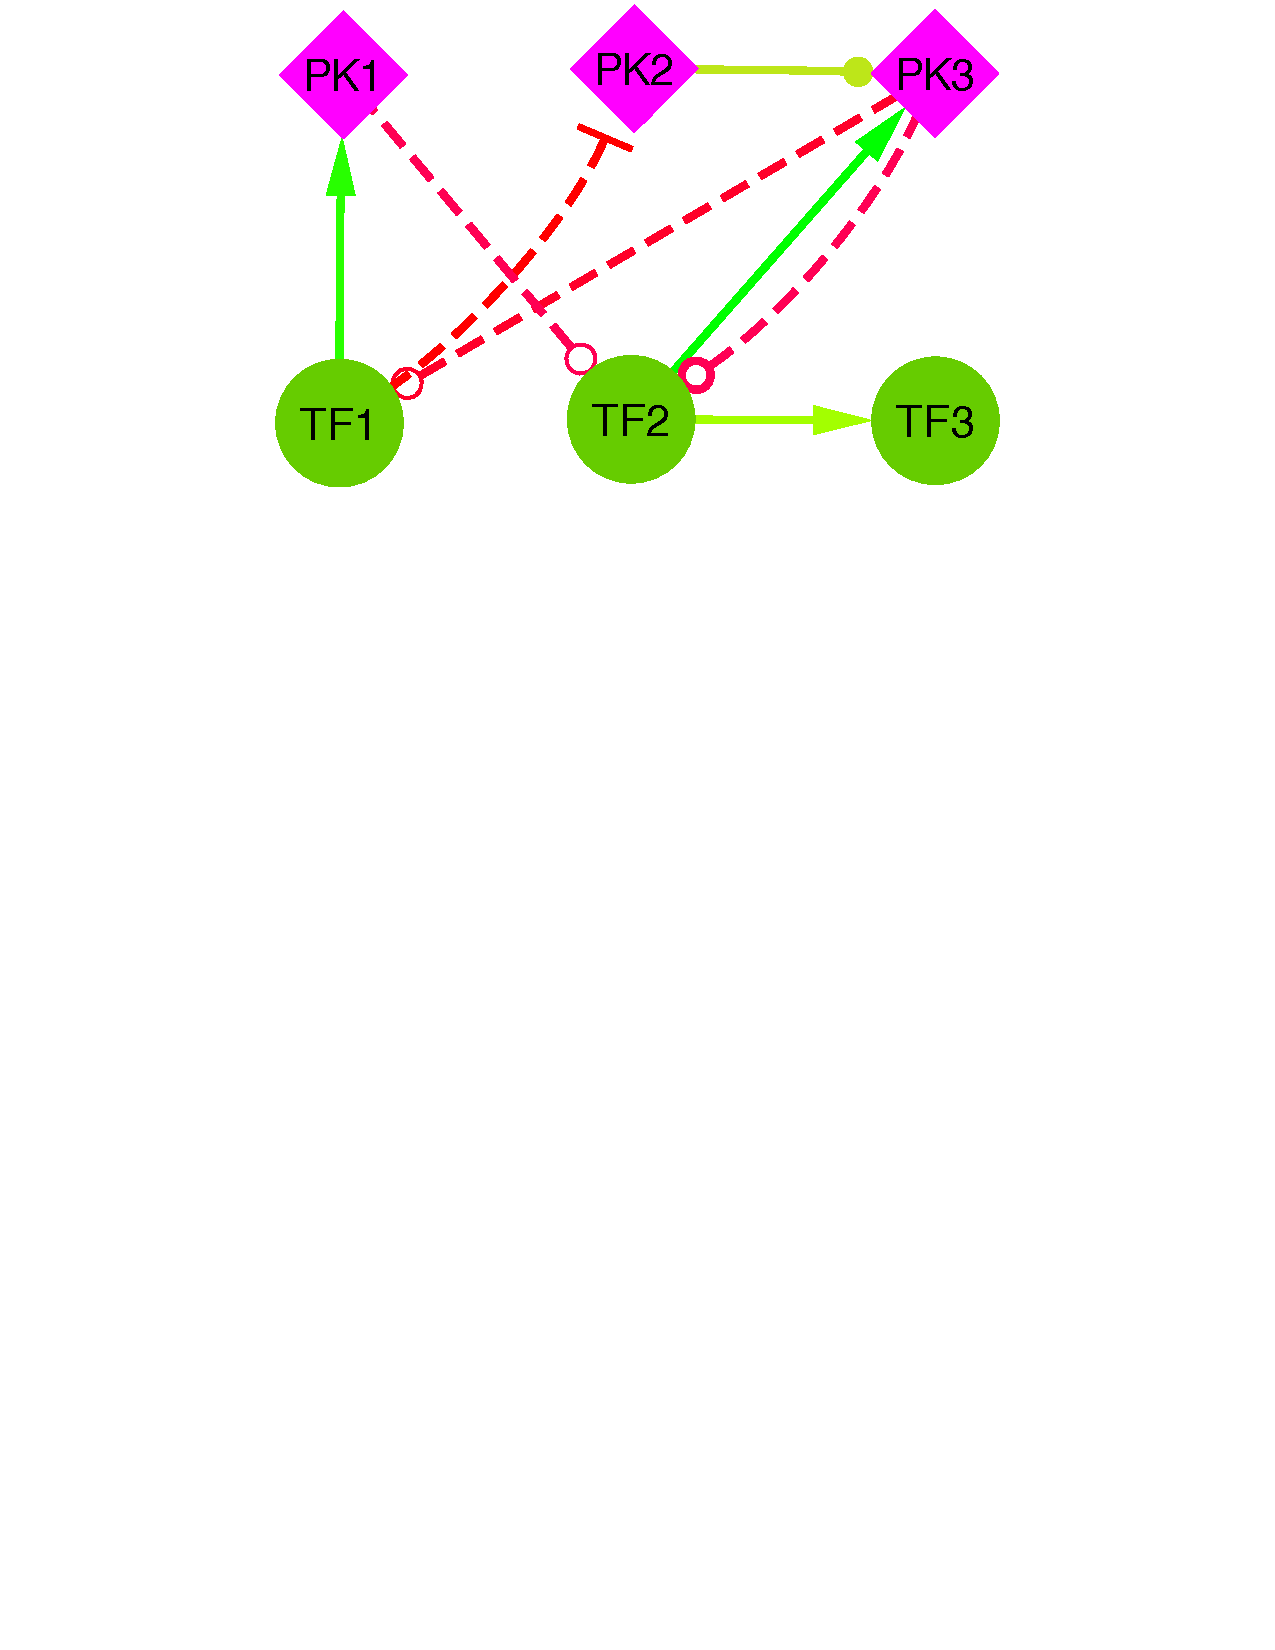
\includegraphics[width=0.8\textwidth]{analysis/fig/cyclic_3.pdf}\label{fig:toy_infer.b}
\end{subfigure}
\vskip\baselineskip
\begin{subfigure}[b]{0.4\textwidth}\centering\caption{}
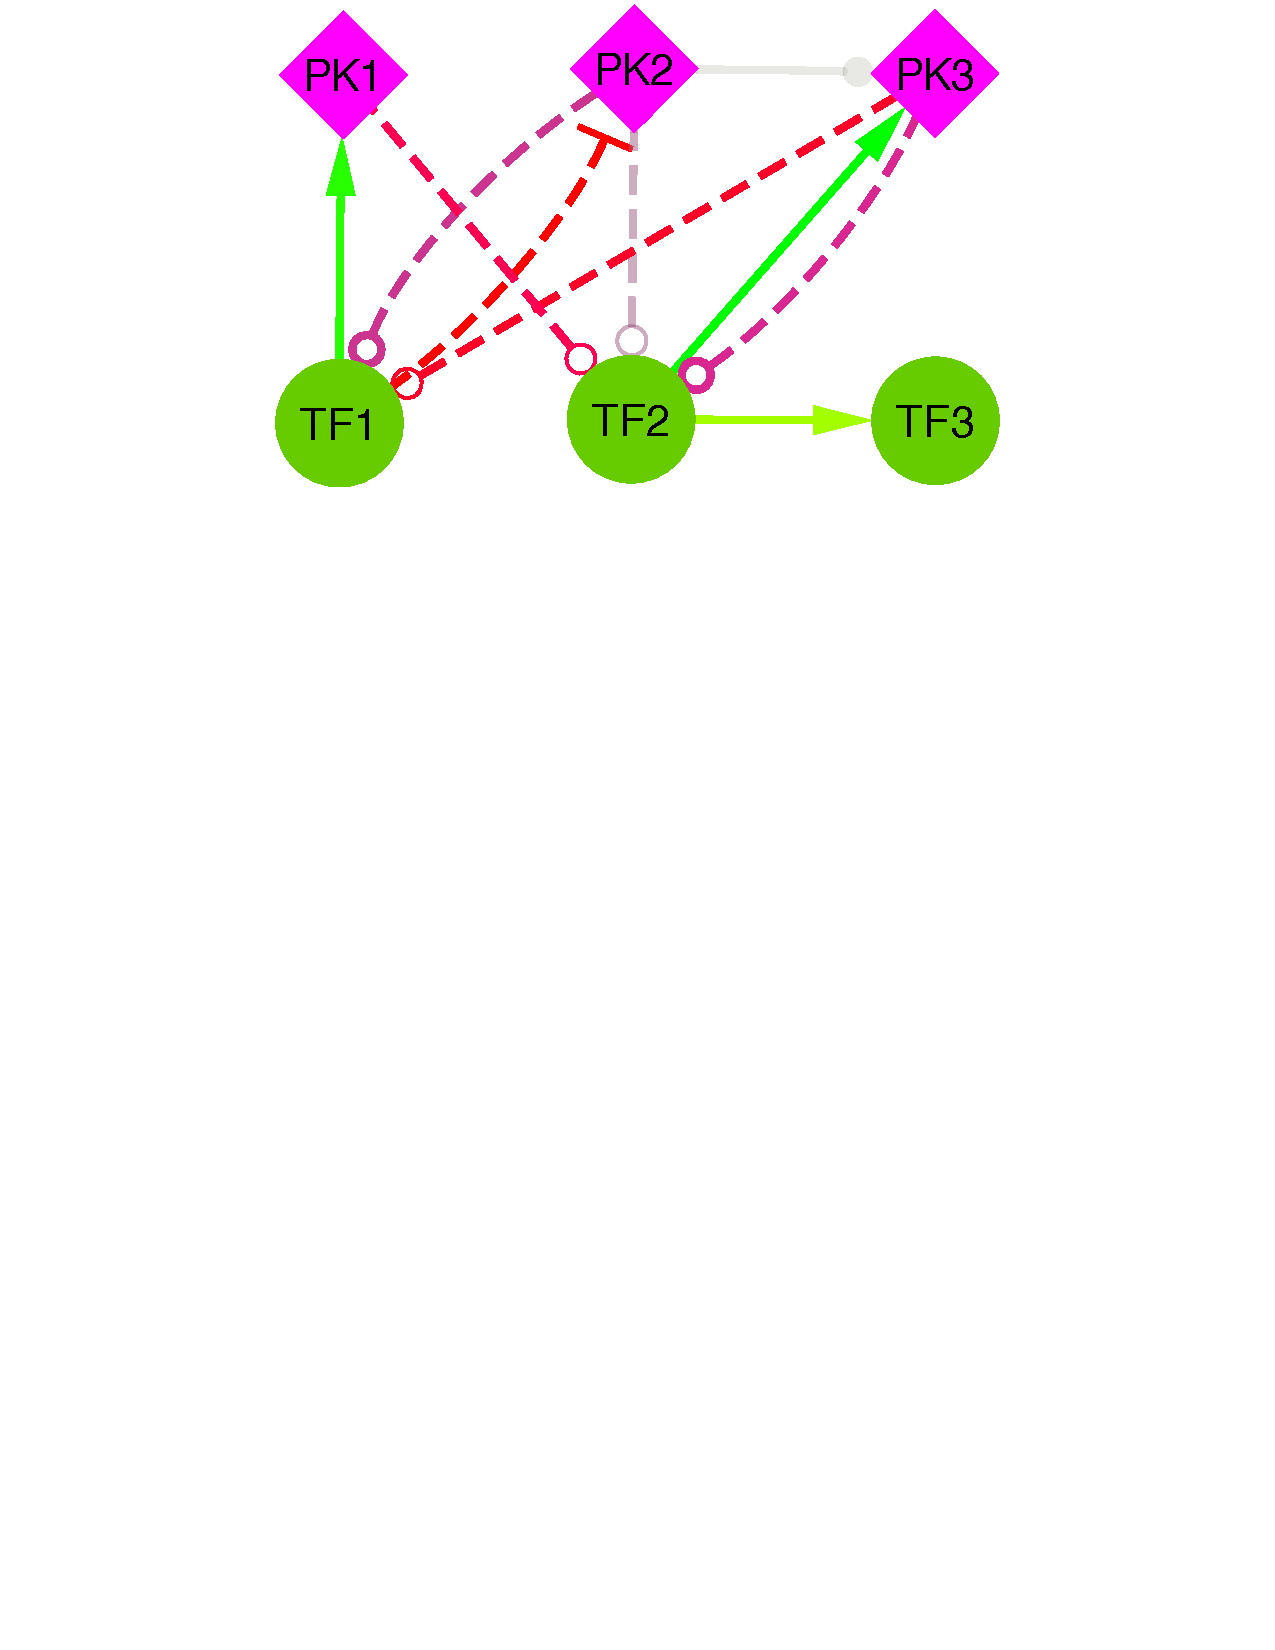
\includegraphics[width=0.8\textwidth]{analysis/fig/cyclic_4.pdf}\label{fig:toy_infer.c}
\end{subfigure}
\quad
\begin{subfigure}[b]{0.4\textwidth}\centering\caption{}
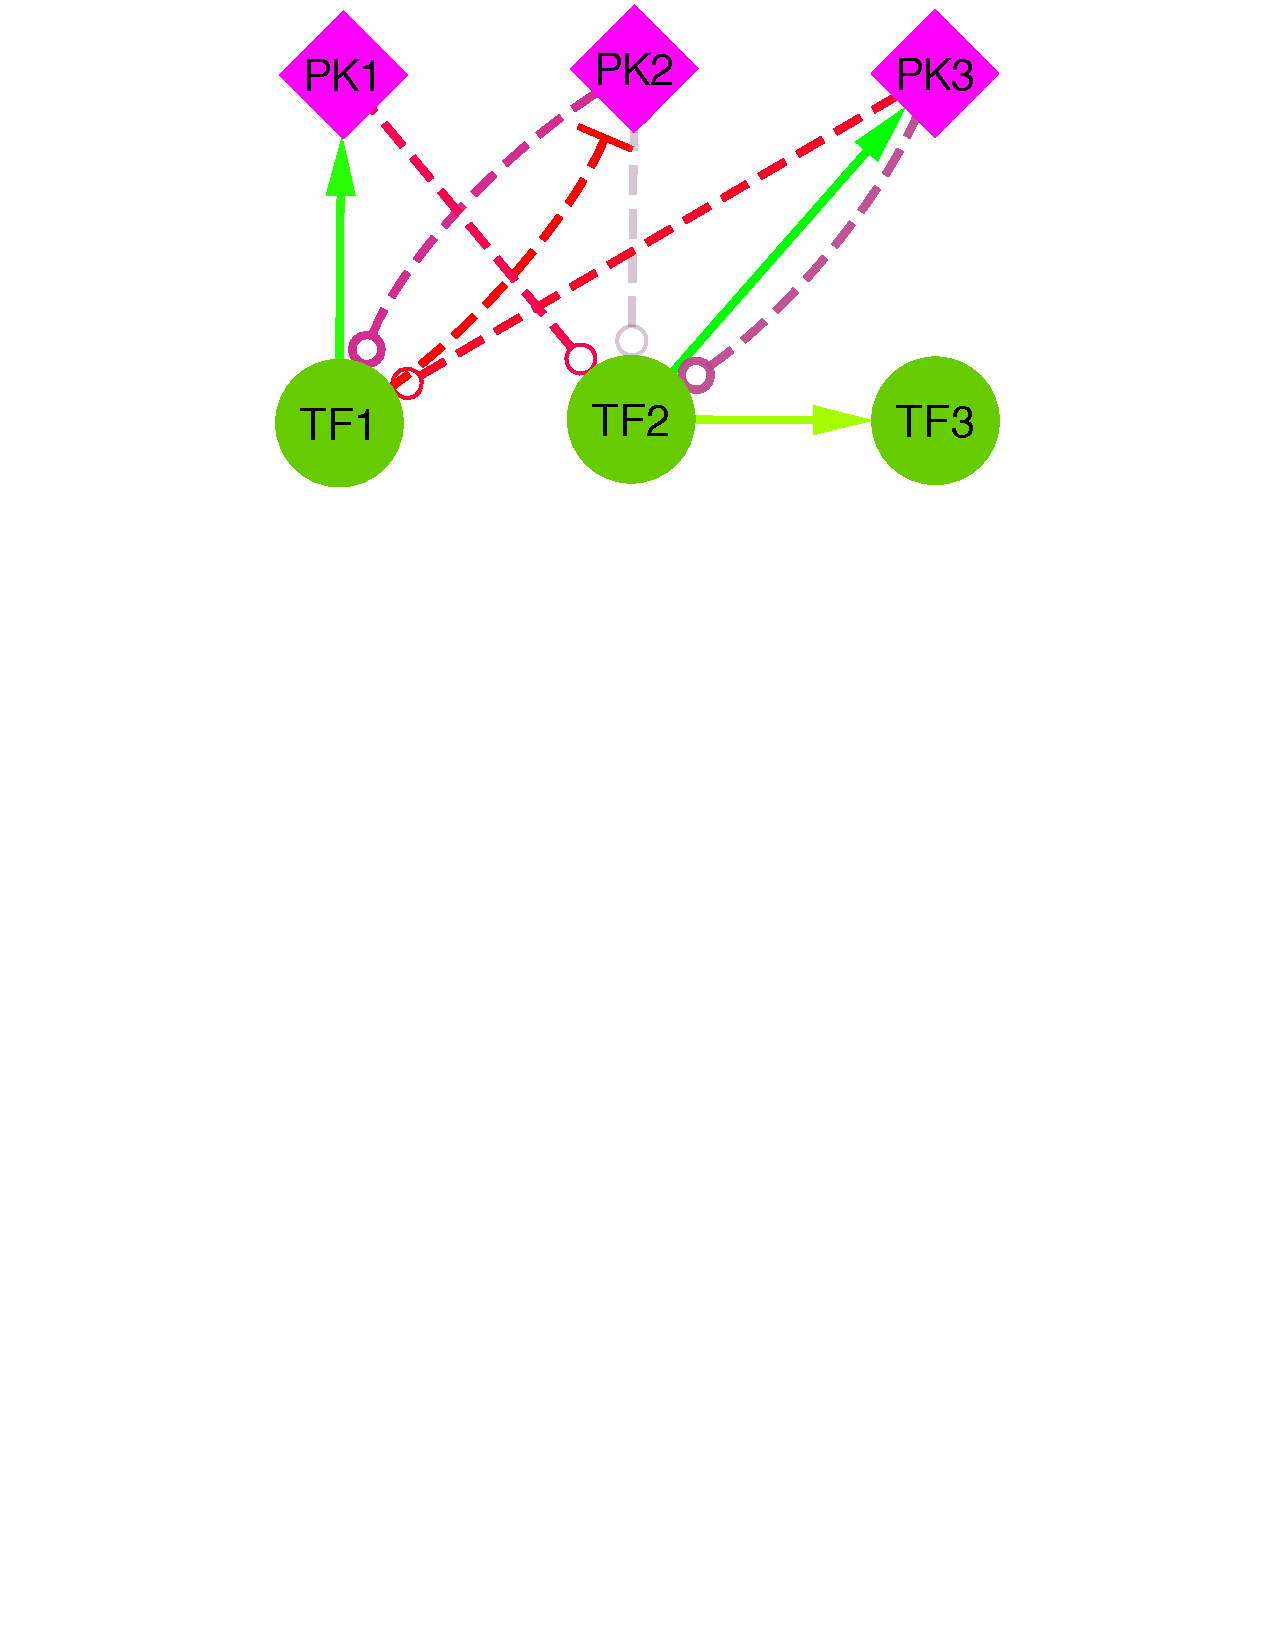
\includegraphics[width=0.8\textwidth]{analysis/fig/cyclic_5.pdf}\label{fig:toy_infer.d}
\end{subfigure}
\vskip\baselineskip
\begin{subfigure}[b]{0.3\textwidth}\centering
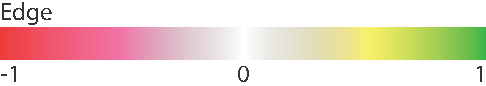
\includegraphics[width=\textwidth]{analysis/fig/edge_legend_cyclic.pdf}
\end{subfigure}
\caption{\textbf{Edge inference.} True $\pk_3\rightarrow\tf_2$ = 0~(\text{a}), -0.6~(\text{b}), -0.3~(c), -0.2~(d). $\boldsymbol{e}$-minimization~($\lambda_T=0.01, \lambda_P=0.01$). Simple simulation. }
\label{fig:toy_infer}
\end{figure}

% Node values were simulated on each of the four graphs with approximate convergence using the simple iterative approach~(\autoref{sec:prim}). Edge values were then inferred using the $\boldsymbol{e}$-minimization method with $\lambda_{TF} = 0.01$ and $\lambda_{PK} = 0.01$~(\autoref{sec:equilibrium_model}). The inferred edges are shown in~\autoref{fig:toy_infer} for each of the four graphs produced from varying a single edge value as indicated in~\autoref{fig:toy}.

% First, the leftmost blue edge in~\autoref{fig:toy} is added to the DAG~(the rightmost blue edge has an edge value of zero). We observe that the inference method now detects the effect of $\pk_2$, but it predicts it is a direct edge to $\tf_1$, rather than an indirect effect mediated by $\pk_3$~(\autoref{fig:toy_infer.a}). This is a rational prediction, given that the node value data would be equivalent in a case where an edge from $\pk_2$ to $\tf_1$ was present, with edge value equal to the product of the true edge values from $\pk_2\rightarrow \pk_3$ and $\pk_3\rightarrow \tf_1$.
\end{column}
\end{columns}
\end{frame}

\begin{frame}{Cyclic graphs - favoring PK$\rightarrow$PK vs. PK$\rightarrow$TF}

% Next, we show that if $\pk_3$ were to have more outgoing edges, in this case directly to $\tf_2$, then the inference will predict the $\pk_2\rightarrow \pk_3$ edge correctly~(\autoref{fig:toy_infer.b}). Even though it is still possible to explain the observed effect from $\pk_2$ to $\tf_1$ and $\tf_2$, it is the favored explanation, that the effect is mediated by a single edge from the protein kinase: $\pk_2 \rightarrow \pk_3$ (option A), rather than needing two edges: $\pk_2 \rightarrow \tf_1$ and $\pk_2 \rightarrow \tf_2$ (option B). This is a result of regularization, where by applying an L1-regularization to all parameters~(edge values), we predict the parameters that explains the data with the smallest possible edge values, which reduces the count of edges and promotes sparsity. 

% The balance between the choice of a PK$\rightarrow$TF edge versus a PK$\rightarrow$PK$\rightarrow$TF path, is based on the smallest sum of absolute edge values for each case. We explore this by reducing the edge value for the rightmost blue edge in~\autoref{fig:toy}. We observe that for small values, option B with two edges, $\pk_2 \rightarrow \tf_1$ and $\pk_2 \rightarrow \tf_2$, will be favorable~(\autoref{fig:toy_infer.d}), and for a certain threshold both option A and B will be equally likely, at which point all paths are inferred to have a combined effect~(\autoref{fig:toy_infer.c}). The threshold is found when the L1-regularization are the same for option A and B, given that $\boldsymbol{e}$ is equal for both options~(\autoref{eq:loss_e}). We formulate the L1-norm cost for all paths from $\pk_2$ in option A and B:
Option A: $\pk_{}\rightarrow\pk_{}$ \\
Option B: $\pk_{}\rightarrow\tf_{}$ \\
Norms differentiating loss for option A and B
\begin{subequations}
\label{eq:toy_l1}
\begin{align}
L1_{\pk_2\rightarrow\pk_3}
&=
|w_{\pk_2\rightarrow\pk_3}^{(\text{A})}|
\\
L1_{\pk_2\rightarrow \{\tf_1,\tf_2\}}
&=
|w_{\pk_2\rightarrow \tf_1}^{(\text{B})}| + |w_{\pk_2\rightarrow \tf_2}^{(\text{B})}|
\label{eq:toy_l1.B}
\end{align}
\end{subequations}


% Superscripts $(\text{A})$ and $(\text{B})$ indicates the option, where a weight parameters $w^{(\text{A})}$ will be nonzero for option A and $w^{(\text{B})}$ nonzero for option B. If the effects from $\pk_2$ to both $\tf_1$ and $\tf_2$ are perfectly captured for option A and B, then the total effects can be written using notation similar to~\autoref{sec:eberhardt}:

Effects from $\pk_2$ to \textcolor{tf}{TFs} are equal for choice A and B
\begin{subequations}
\label{eq:toy_t}
\begin{align}
t(\pk_2 \rightsquigarrow \tf_1)
&=
w_{\pk_2\rightarrow \pk_3}^{(\text{A})} \cdot
t(\pk_3 \rightsquigarrow \tf_1)
=
w_{\pk_2\rightarrow \pk_3}^{(\text{A})} \cdot 
w_{\pk_3\rightarrow \tf_1}
\\
&=
w_{\pk_2\rightarrow \tf_1}^{(\text{B})}
\\
t(\pk_2 \rightsquigarrow \tf_2)
&=
w_{\pk_2\rightarrow \pk_3}^{(\text{A})} \cdot t(\pk_3 \rightsquigarrow \tf_2)
=
w_{\pk_2\rightarrow \pk_3}^{(\text{A})} \cdot w_{\pk_3\rightarrow \tf_2}
\\
&=
w_{\pk_2\rightarrow \tf_2}^{(\text{B})}
\end{align}
\end{subequations}

\end{frame}
\begin{frame}{Cyclic graphs - favoring PK$\rightarrow$PK vs. PK$\rightarrow$TF}


% By summing~\autoref{eq:toy_t} we can formulate $L1_{\pk_2 \rightarrow \pk_3}$:

\begin{subequations}
\begin{align}
|t(\pk_2 \rightsquigarrow \tf_1)| + |t(\pk_2 \rightsquigarrow \tf_2)| &=
|w_{\pk_2\rightarrow \pk_3}^{(\text{A})}|
\left(|w_{\pk_3\rightarrow \tf_1}| + |w_{\pk_3\rightarrow \tf_2}|\right)
\\
&= |w_{\pk_2\rightarrow \tf_1}^{(\text{B})}| + |w_{\pk_2\rightarrow \tf_2}^{(\text{B})}|
\\
\implies
L1_{\pk_2 \rightarrow \pk_3}
&=
\frac
{|w_{\pk_2\rightarrow \tf_1}^{(\text{B})}| + |w_{\pk_2\rightarrow \tf_2}^{(\text{B})}|}
{|w_{\pk_3\rightarrow \tf_1}| + |w_{\pk_3\rightarrow \tf_2}|}
\\
&=
\frac{
L1_{\pk_2\rightarrow\{\tf_1,\tf_2\}}
}{
|w_{\pk_3\rightarrow\tf_1}| + |w_{\pk_3\rightarrow \tf_2}|
}
\end{align}
\end{subequations}

% This means that option A has the lowest L1-norm, and is inferred, when edges from $\pk_3$ sum to more than 1, option B is inferred when they sum to less than 1, and both options are combined when edges from $\pk_3$ sum to 1. It is demonstrated in~\autoref{fig:toy_infer.b}, \ref{fig:toy_infer.c}, and \ref{fig:toy_infer.d}, where the sums are $|-0.7| + |-0.6| = 1.2$, $|-0.7| + |-0.3| = 1.0$, and $|-0.7| + |-0.2| = 0.9$.

Option A favored when $|w_{\pk_3\rightarrow \tf_1}| + |w_{\pk_3\rightarrow \tf_2}| < 1$

General formulations (more norms may be compared):

% So, if the data can be perfectly modeled in either case considered, then for an edge $\text{PK}_j \rightarrow \text{PK}_i$ and for the case of direct edges from $\text{PK}_j$ to each regulated $\text{TF}_k$ the generalized L1-norms will be

\begin{subequations}
\begin{align}
L1_{\text{PK}_j \rightarrow \text{PK}_i}
&=
\frac{
L1_{\text{PK}_j \rightarrow \{\text{TF}_k\}}
}{
\sum_k |t(\text{PK}_i \rightsquigarrow \text{TF}_k)|
}
\\
L1_{\text{PK}_j \rightarrow \{\text{TF}_k\}}
&=
\sum_k |w_{\text{PK}_j \rightarrow \text{TF}_k}|
\end{align}
\end{subequations}

% Where $k$ indexes all TFs that are regulated by $\text{PK}_j$ through a directed path of PKs.

% For a more complicated graph, there can be many other L1-norms that the model will compare, than the two exemplified here.
% In general, applying the L1-regularization indiscriminately on each parameter will make the model favor paths with fewer edges. The smaller the parameters found for a dataset, the rarer PK$\rightarrow$PK edges will be inferred. The parameters will usually be less than 1 since parameters above 1 easily leads to divergence in the model.
\end{frame}
\begin{frame}{Loss function favoring longer cascades}
\label{sec:cascade_loss}
\begin{columns}
\begin{column}{0.65\textwidth}

% Other loss functions can be considered to treat longer cascades more favorably. One idea would be to replace the use of the regularization hyperparameter $\lambda_{PK}$ with a regularization strength for $\text{PK}\rightarrow\text{TF}$ and a smaller one for $\text{PK}\rightarrow\text{PK}$ edges, however this creates loops among the PKs to artificially strengthen the $\text{PK}\rightarrow\text{TF}$ edges~(not shown).

% A solution to consider is replacing the L1-regularization of PK edges with a loss based on a sum of effects $t(\text{PK}_j\rightsquigarrow\text{TF}_i)$ that each PK has through all its cascades. This is done in a similar fashion to the classification of detectable nodes~(\autoref{sec:unobservable}). 

PK edge norm = total effect on TFs
\begin{equation}
\label{eq:pk_effect}
\boldsymbol{l}_{\text{cas}} =
\sum_{k=1}^K {(|W|I_P)^\trans}^k
(I_T \boldsymbol{1} )
\end{equation}

% Here, $|W|$ is used for indication of element-wise absolute values of $W$. $K$ can be found similarly to described in~\autoref{sec:unobservable}, however due to noise in the weights while training it is best to have an upper bound for $K$, which can be chosen conservatively since the only downside to using a too large $K$ is computational cost. $W$ has to be square. If there are more measured genes than knockouts, we use $I_SW$ instead, where $I_S$ is an identity matrix with dimensions $(N_T + N_P) \times N$, and $N$ is the total number of measured genes.

% If $I-(|W|I_P)^\trans$ is invertible, we can get rid of $K$ from~\autoref{eq:pk_effect}, as it was done in~\autoref{sec:unobservable}.
for $K\rightarrow\infty$
\begin{equation}
\boldsymbol{l}_{\text{cas}} =
\left(
\sum_{k=1}^\infty {(|W|I_P)^\trans}^k
\right)
(I_T \boldsymbol{1} )
=
\left(
I-(|W|I_P)^\trans
\right)^{-1}
(I_T \boldsymbol{1} )
\end{equation}

% We define a new loss function that favors longer cascades:

\begin{equation}
\mathcal{L}_\text{cas} =
\sum_{i=1}^N e_i^2 + \lambda_T \sum_{j \in \text{TF}} \sum_{i=1}^N |w_{ij}| + \lambda_P \sum_{i=0}^{N_T + N_P} \left(
\sum_{j \in \text{PK}} |w_{ij}|
+ l_i^{(\text{cas})}
\right)
\label{eq:loss_cas}
\end{equation}

% Here, $\boldsymbol{l}_{\text{cas}}$ and the L1-norm regularization term used in~\autoref{eq:loss_e} are summed, where  $l_i^{(\text{cas})}$ is the $i$-th element of $\boldsymbol{l}_\text{cas}$.

\end{column}
\begin{column}{0.35\textwidth}
\begin{figure}[ht]
\centering
\begin{subfigure}[b]{0.7\textwidth}\centering
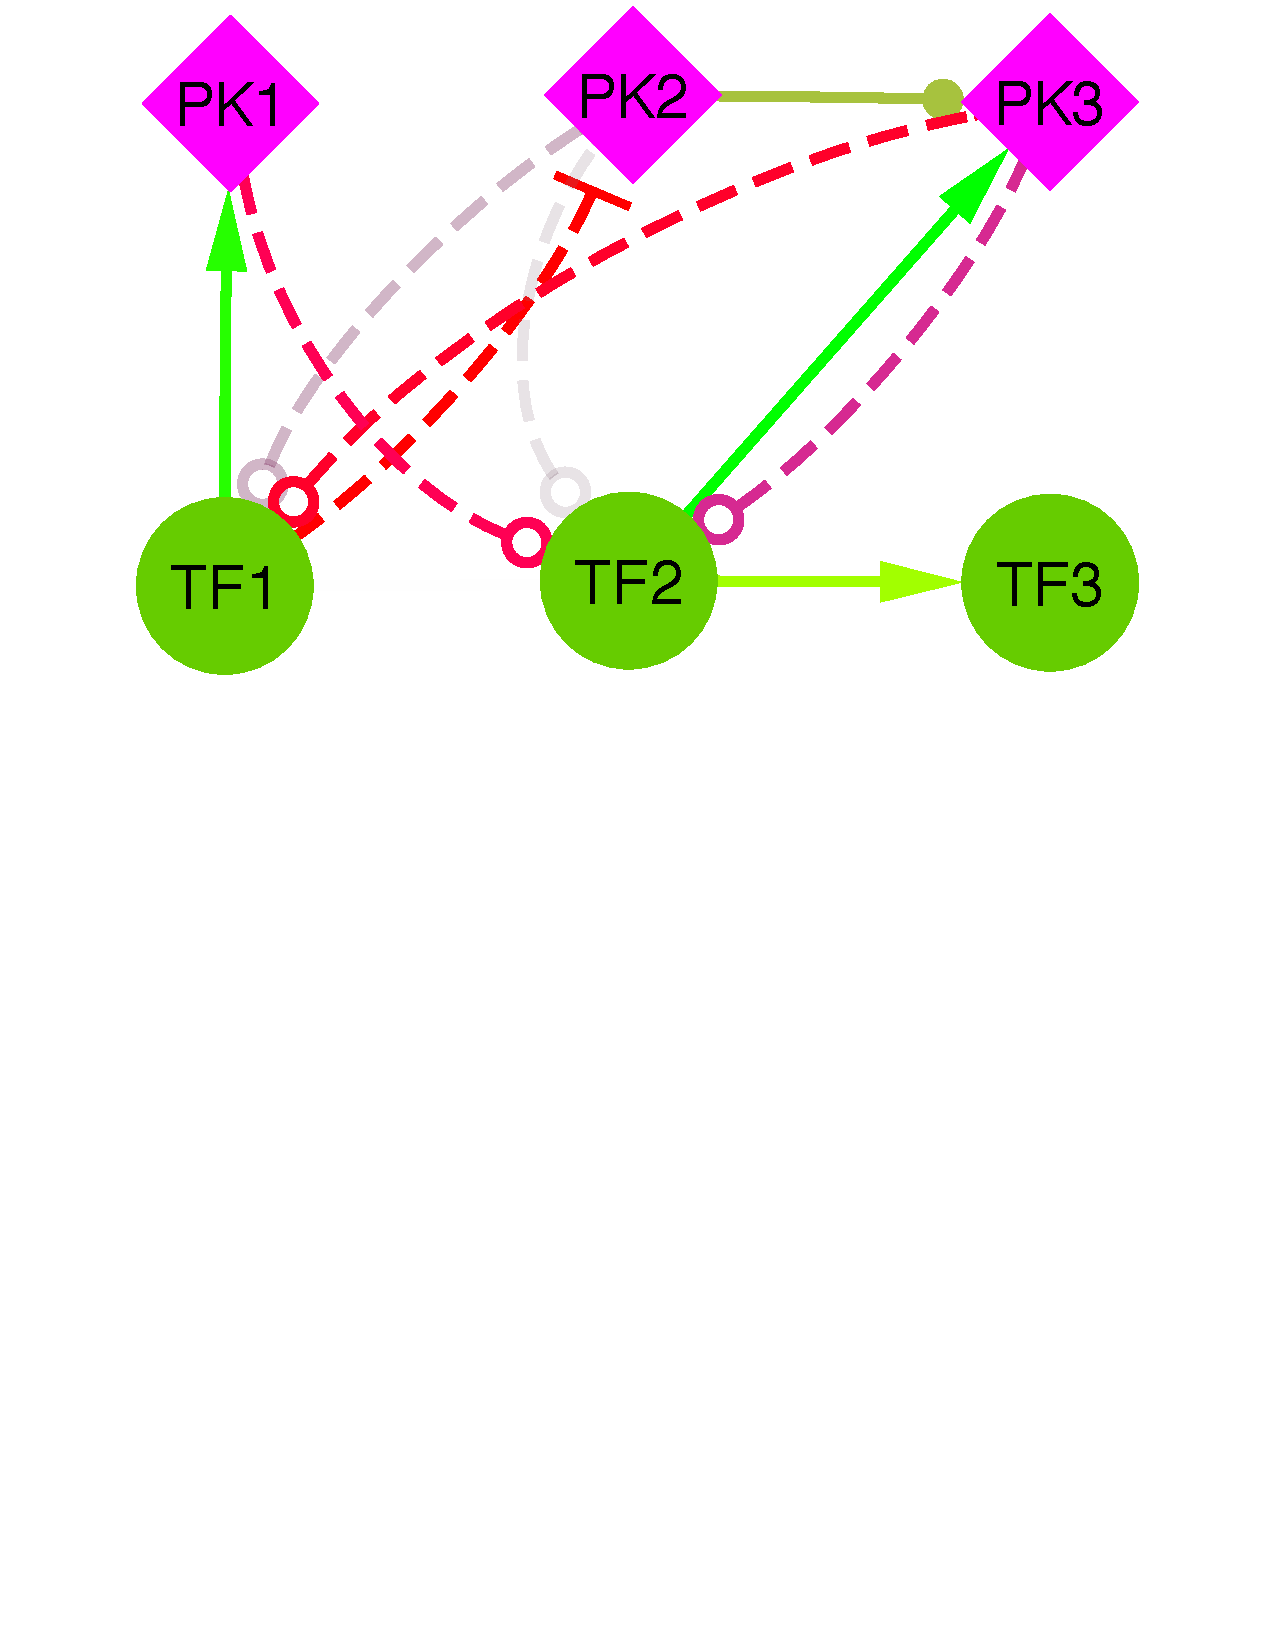
\includegraphics[width=\textwidth]{analysis/fig/cyclic_4_cas.pdf}
\end{subfigure}
\vskip\baselineskip
\begin{subfigure}[b]{0.5\textwidth}\centering
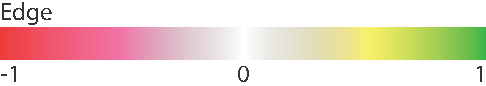
\includegraphics[width=\textwidth]{analysis/fig/edge_legend_cyclic.pdf}
\end{subfigure}
\caption{\textbf{Correcting inference.} Inference from~fig.~\ref{fig:toy_infer.c} using $\mathcal{L}_\text{cas}$~(eq.~\ref{eq:loss_cas}) instead of $\mathcal{L}_{\boldsymbol{e}}$~(eq.~\ref{eq:loss_e}).
$\lambda_T=0.01$, $\lambda_P=0.01$. }
\label{fig:toy_cas}
\end{figure}

% The loss function was tested for edge inference otherwise identical to the procedure for~\autoref{fig:toy_infer.c}, for instance instance by using $\lambda_T=0.01$ and $\lambda_P=0.01$ as before. The inferred edge values are shown in~\autoref{fig:toy_cas}. We see that the change in loss function has corrected the inference to favor the $\pk_2\rightarrow\pk_3$ edge, which has been referred to as option A.

% The remaining work in this section describes inference attempts using standard L1-regularization. $\mathcal{L}_\text{cas}$ has yet to be tested for possibilities of improving performance on larger networks.
\end{column}
\end{columns}
\end{frame}

\begin{frame}{Edge inference on DREAM networks - 10 nodes}
\label{sec:dream_results}
\begin{columns}
\begin{column}{0.4\textwidth}
% The DREAM data goldstandards for the five 10-node graphs were used for simulation of node values using the simple iteration method~(\autoref{sec:prim}), after randomly assigning uniform edge strengths in range~$[-1,1]$.

\begin{figure}[ht]
    \centering
    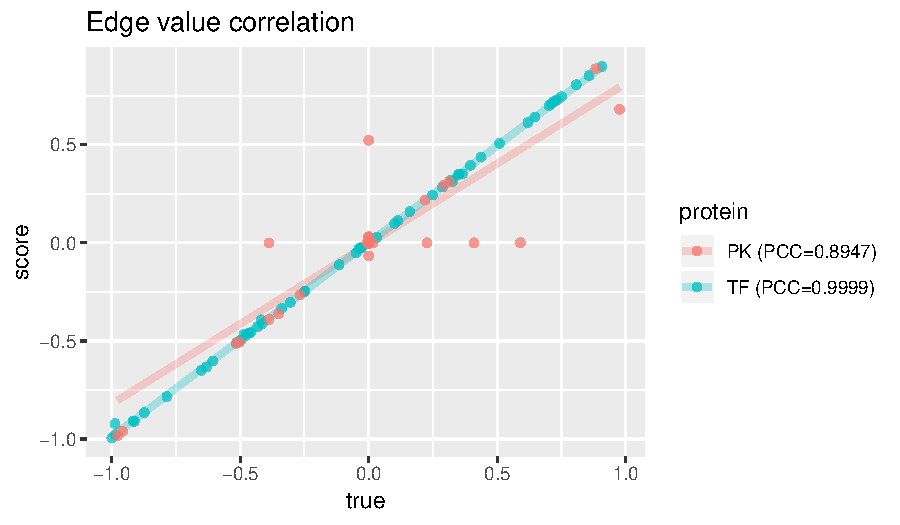
\includegraphics[width=\textwidth]{analysis/fig/edge_cor_10.pdf}
    \caption{\textbf{Predicted vs. true edge values.} 5 10-node networks. Simple simulation. }
    \label{fig:edge_value_cor_10}
\end{figure}

% The resulting inferred edge values for a single edge inference attempt on each graph are compared to the true edge values~(\autoref{fig:edge_value_cor_10}). There are three undetectable edges for the five graphs. They are included in this plot and all have a score of zero. The points along the line \texttt{score}=\texttt{true} are edges where the weight~(score) accurately predicts the true edge strength used for node value simulation. A few outlier protein kinase edges can be seen as being misclassified. Most values are found in the point (0,0) which are all non-edges correctly classfied as non-edges (true negatives). The purpose of the plot is to show that for very simple cases the edges are not only found, but their exact edge value is also inferred. It also shows that there is 1 false positive and 1 false negative of the 15 detectable PK edges, and that inference on TF edges are perfect in this simple example.
\begin{itemize}
    \item Predicted edge values accurate to truth
    \item LLC fails for kinases
\end{itemize}
\end{column}
\begin{column}{0.6\textwidth}

\begin{figure}[ht]
\centering
\begin{subfigure}[b]{0.49\textwidth}\centering\caption{}
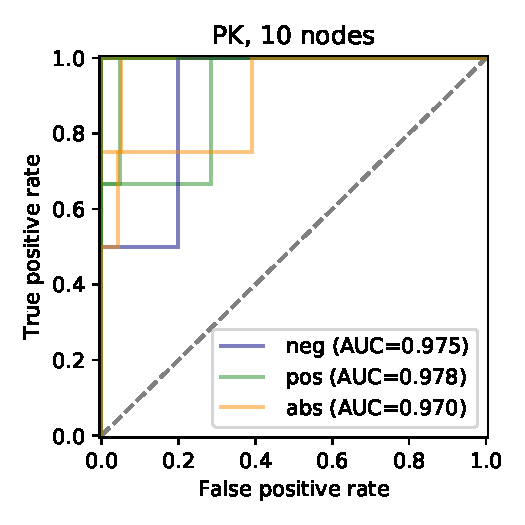
\includegraphics[width=\textwidth]{analysis/fig/roc_pk_10.pdf}
\end{subfigure}
\hfill
\begin{subfigure}[b]{0.49\textwidth}\centering\caption{}
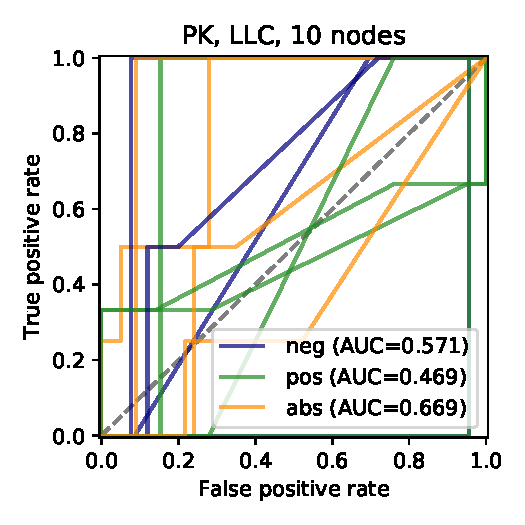
\includegraphics[width=\textwidth]{analysis/fig/roc_pk_llc_10.pdf}
\end{subfigure}
\caption{\textbf{ROC curves for 5 10-node networks.} $\boldsymbol{e}$-minimization~(a) and LLC~\cite{EberhardtLLC}~(b) on PK edges. neg: inference of negative edges, pos: positive, abs: ignoring sign. AUCs are micro averaged.}
\label{fig:roc_pk_10}
\end{figure}

% The inference can also be described with ROC curves for outgoing PK edges in each individual graph~(\autoref{fig:roc_pk_10}). Inference of the presence or absence of edges from transcription factors to genes were perfect on this simple simulation~(AUC=1). For protein kinases the inference is less trivial, as we see that AUCs drops below perfect scores. Note that most curves are perfect, and that the ones not following the path (0,0)$\rightarrow$(0,1)$\rightarrow$(1,1) are a minority. This is also apparent from the AUC scores, which are close to perfect. The ROC curves are also shown for inference performed using the LLC method~\cite{EberhardtLLC}. Since it infers linear direct causal interactions and it fails to classify presence and absence of outgoing PK edges based on their indirect effects on the observed node values.
\end{column}
\end{columns}
\end{frame}

\begin{frame}{Edge inference on DREAM networks - 100 nodes}
% This comparison is biased towards the equilibrium method since the data simulation is performed with the same equations that are used for the $\boldsymbol{e}$-minimization inference, so to increase realism and fairness of performance testing we move on to the larger 100-node graphs where we will use the more realistic GeneNetWeaver kinase extension code for simulation of observable node values.
\begin{figure}[ht]
\centering
\begin{subfigure}[b]{0.24\textwidth}\centering\caption{}
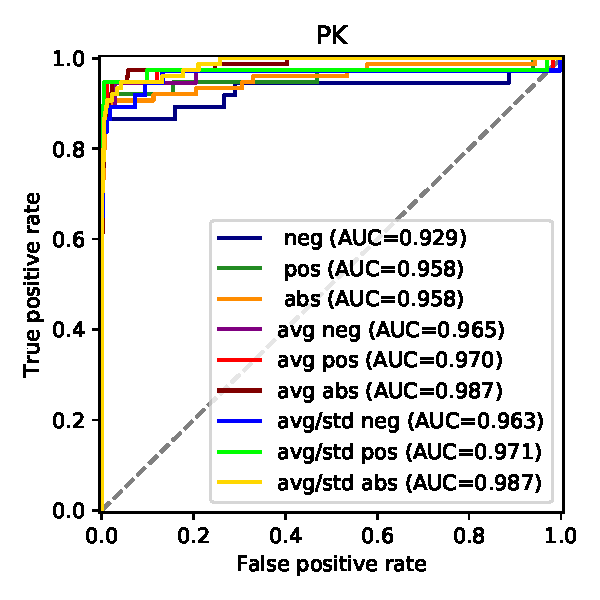
\includegraphics[width=\textwidth]{analysis/fig/roc_pk_prim.pdf}
\end{subfigure}
\hfill
\begin{subfigure}[b]{0.24\textwidth}\centering\caption{}
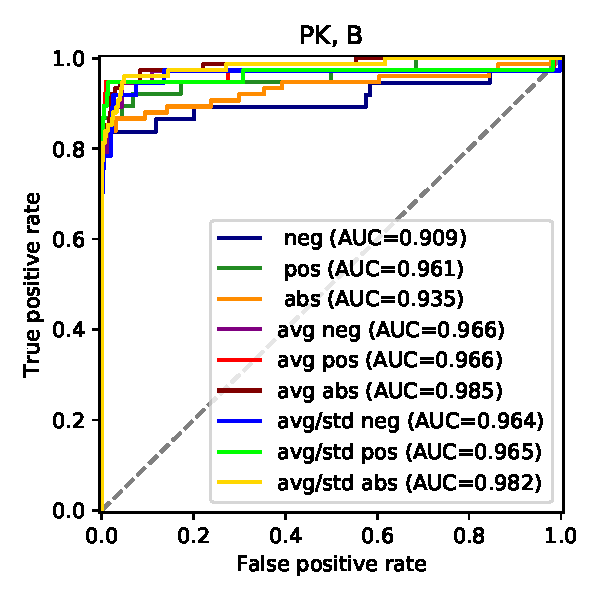
\includegraphics[width=\textwidth]{analysis/fig/roc_pk_prim_B.pdf}
\end{subfigure}
\hfill
\begin{subfigure}[b]{0.24\textwidth}\centering\caption{}
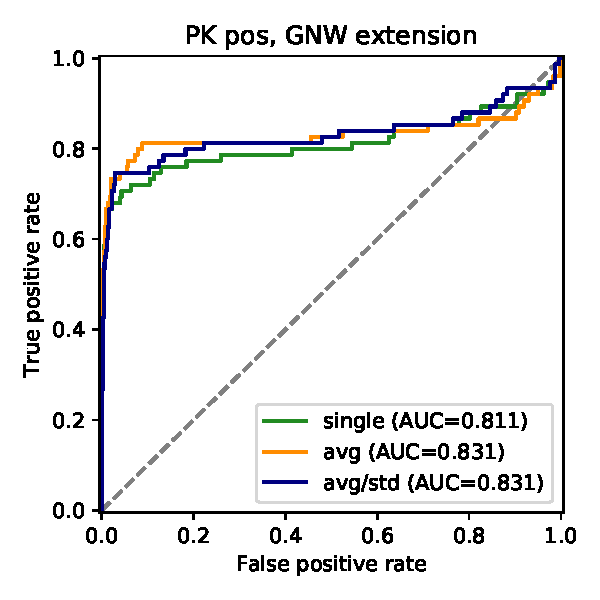
\includegraphics[width=\textwidth]{analysis/fig/roc_pk_gnw_pos.pdf}\label{fig:micro_average.c}
\end{subfigure}
\hfill
\begin{subfigure}[b]{0.24\textwidth}\centering\caption{}
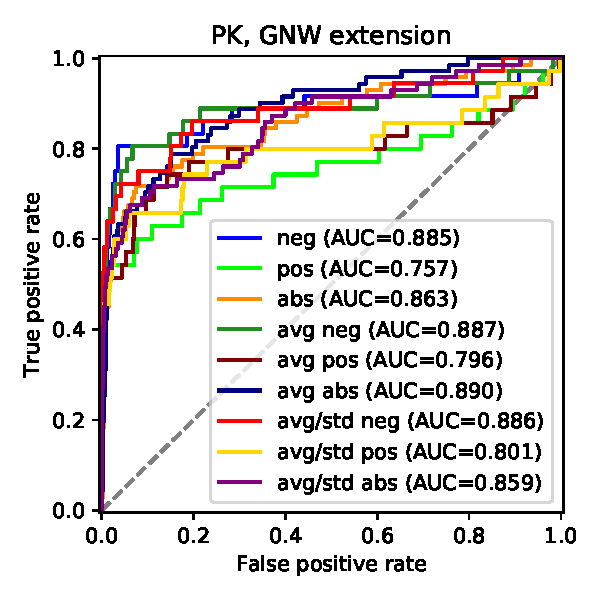
\includegraphics[width=\textwidth]{analysis/fig/roc_pk_gnw.pdf}\label{fig:micro_average.d}
\end{subfigure}
\caption{\textbf{ROC curves for PK edge inference.} $\boldsymbol{e}$-minimization~(a,c,d) and $B$-method~(b). Simple simulation~(a,b), and GeneNetWeaver extension~(c,d). True PK edges all positive~(c) or signed~(d). neg: inference on negative edges. pos: positive. abs: ignoring sign. avg: score = avg. $w$ from 20 runs. avg/std: score = avg./std. $w$, other: score = $w$. }
\label{fig:micro_average}
\end{figure}
$\ge 80 \%$ most prominent edges inferred perfectly
% Edge inference was tested on the five 100-node graphs from DREAM4. The simulations were either performed using the simple iteration method~(\autoref{sec:prim}) or the GeneNetWeaver kinase extension method~(\autoref{sec:gnw_extension}). TF inference was almost perfect with AUC=0.992 for detection of presence or absence of edge, which can be seen in the appendix~(\autoref{fig:gnw_each.a}). The ROC curves, shown in~\autoref{fig:micro_average}, are evaluated on comparisons of inferred and true edges, combined of all five graphs~(microaverage). Individual graphs for individual runs can be seen in~\autoref{app:roc} with equivalent AUC scores.
% Data created with the GNW extension were either simulated where true outgoing PK edges were restricted to a uniform distribution with range~$[0,1]$, or without sign restriction. ROC curves for performance of inference on the former is in~\autoref{fig:micro_average.c}, and the latter in~\autoref{fig:micro_average.d}. The reason for restricting the kinase interaction to positive values are based on the kinase model of regulation~(\autoref{sec:gnw_extension}), which builds on a model of phosphorylation regulation involving only protein kinases with positive interactions~(\autoref{sec:Heinrich}). From the ROC curves it is clear that allowing negative outgoing protein kinase edges does not seem to worsen performance of inference. The negative outgoing protein kinase edges can be seen as a dephosphorylation of the target protein, since $\phi_i$ and $y_i$ from~\autoref{sec:gnw_extension} describes phosphorylation values, and not a general activity concept. It shows that the simulation code and method is robust in allowing for dephosphorylation interactions between specific proteins, rather than only as a background decay~$\lambda_i^{(\text{Phos})}$, since the simulations managed to reach approximate convergence and produce similar inference performance to the trials with sign restriction. Phosphatases are often considered as a background effect to let signals decay, due to their low interaction specificity compared to protein kinases. In spite of this, it is useful that direct dephosphorylation can be simulated and inferred since some of the knockouts in the RNA data are phosphatases~(\autoref{sec:yeast_data}).


% The ROC curves shows a quantitative measure of performance but does not show a final inferred network. To select specific edges we choose a threshold. The threshold was chosen as 0.01 which corresponds to approximately accepting 50\% of inferred PK edges across the five graphs with the highet scores, which corresponds to a cutoff at TPR=0.5 in~\autoref{fig:micro_average.c}. The threshold was applied to all five graphs for all edge types, although different threshold for each were found to be optimal. The inferred edges are shown on the graphs~(\autoref{fig:dream_100_infer}). Activation and repression is not indicated, which is the sign of edges from transcription factors. Edges from protein kinases are all activating as per the restriction to elicit phosphorylation and not dephosphorylation. Kinases not connected to any nodes are included next to each graph. The unconnected kinases are the undetectable kinases. The count of undetectable kinases for each graph is 30 minus the "detectable PK nodes" counts listed in~\autoref{tab:dream_data}, since each graph were initially assigned 30 kinases.

% From the plots we get an impression of the intricacy arising from less than 100 nodes. We see that edges inferred can often be trusted, detects many of the true edges, and that false positives for PK edges arises in situations where there would be ambiguity in what regulation to expect, given only the relative gene expressions. An example is the $\text{PK}_{14}\rightarrow\text{PK}_{29}$ edge at the top-right of net 100.4.
\end{frame}

\begin{frame}{Edge inference on DREAM networks - 100 nodes}
\begin{figure}[ht]
    \centering
    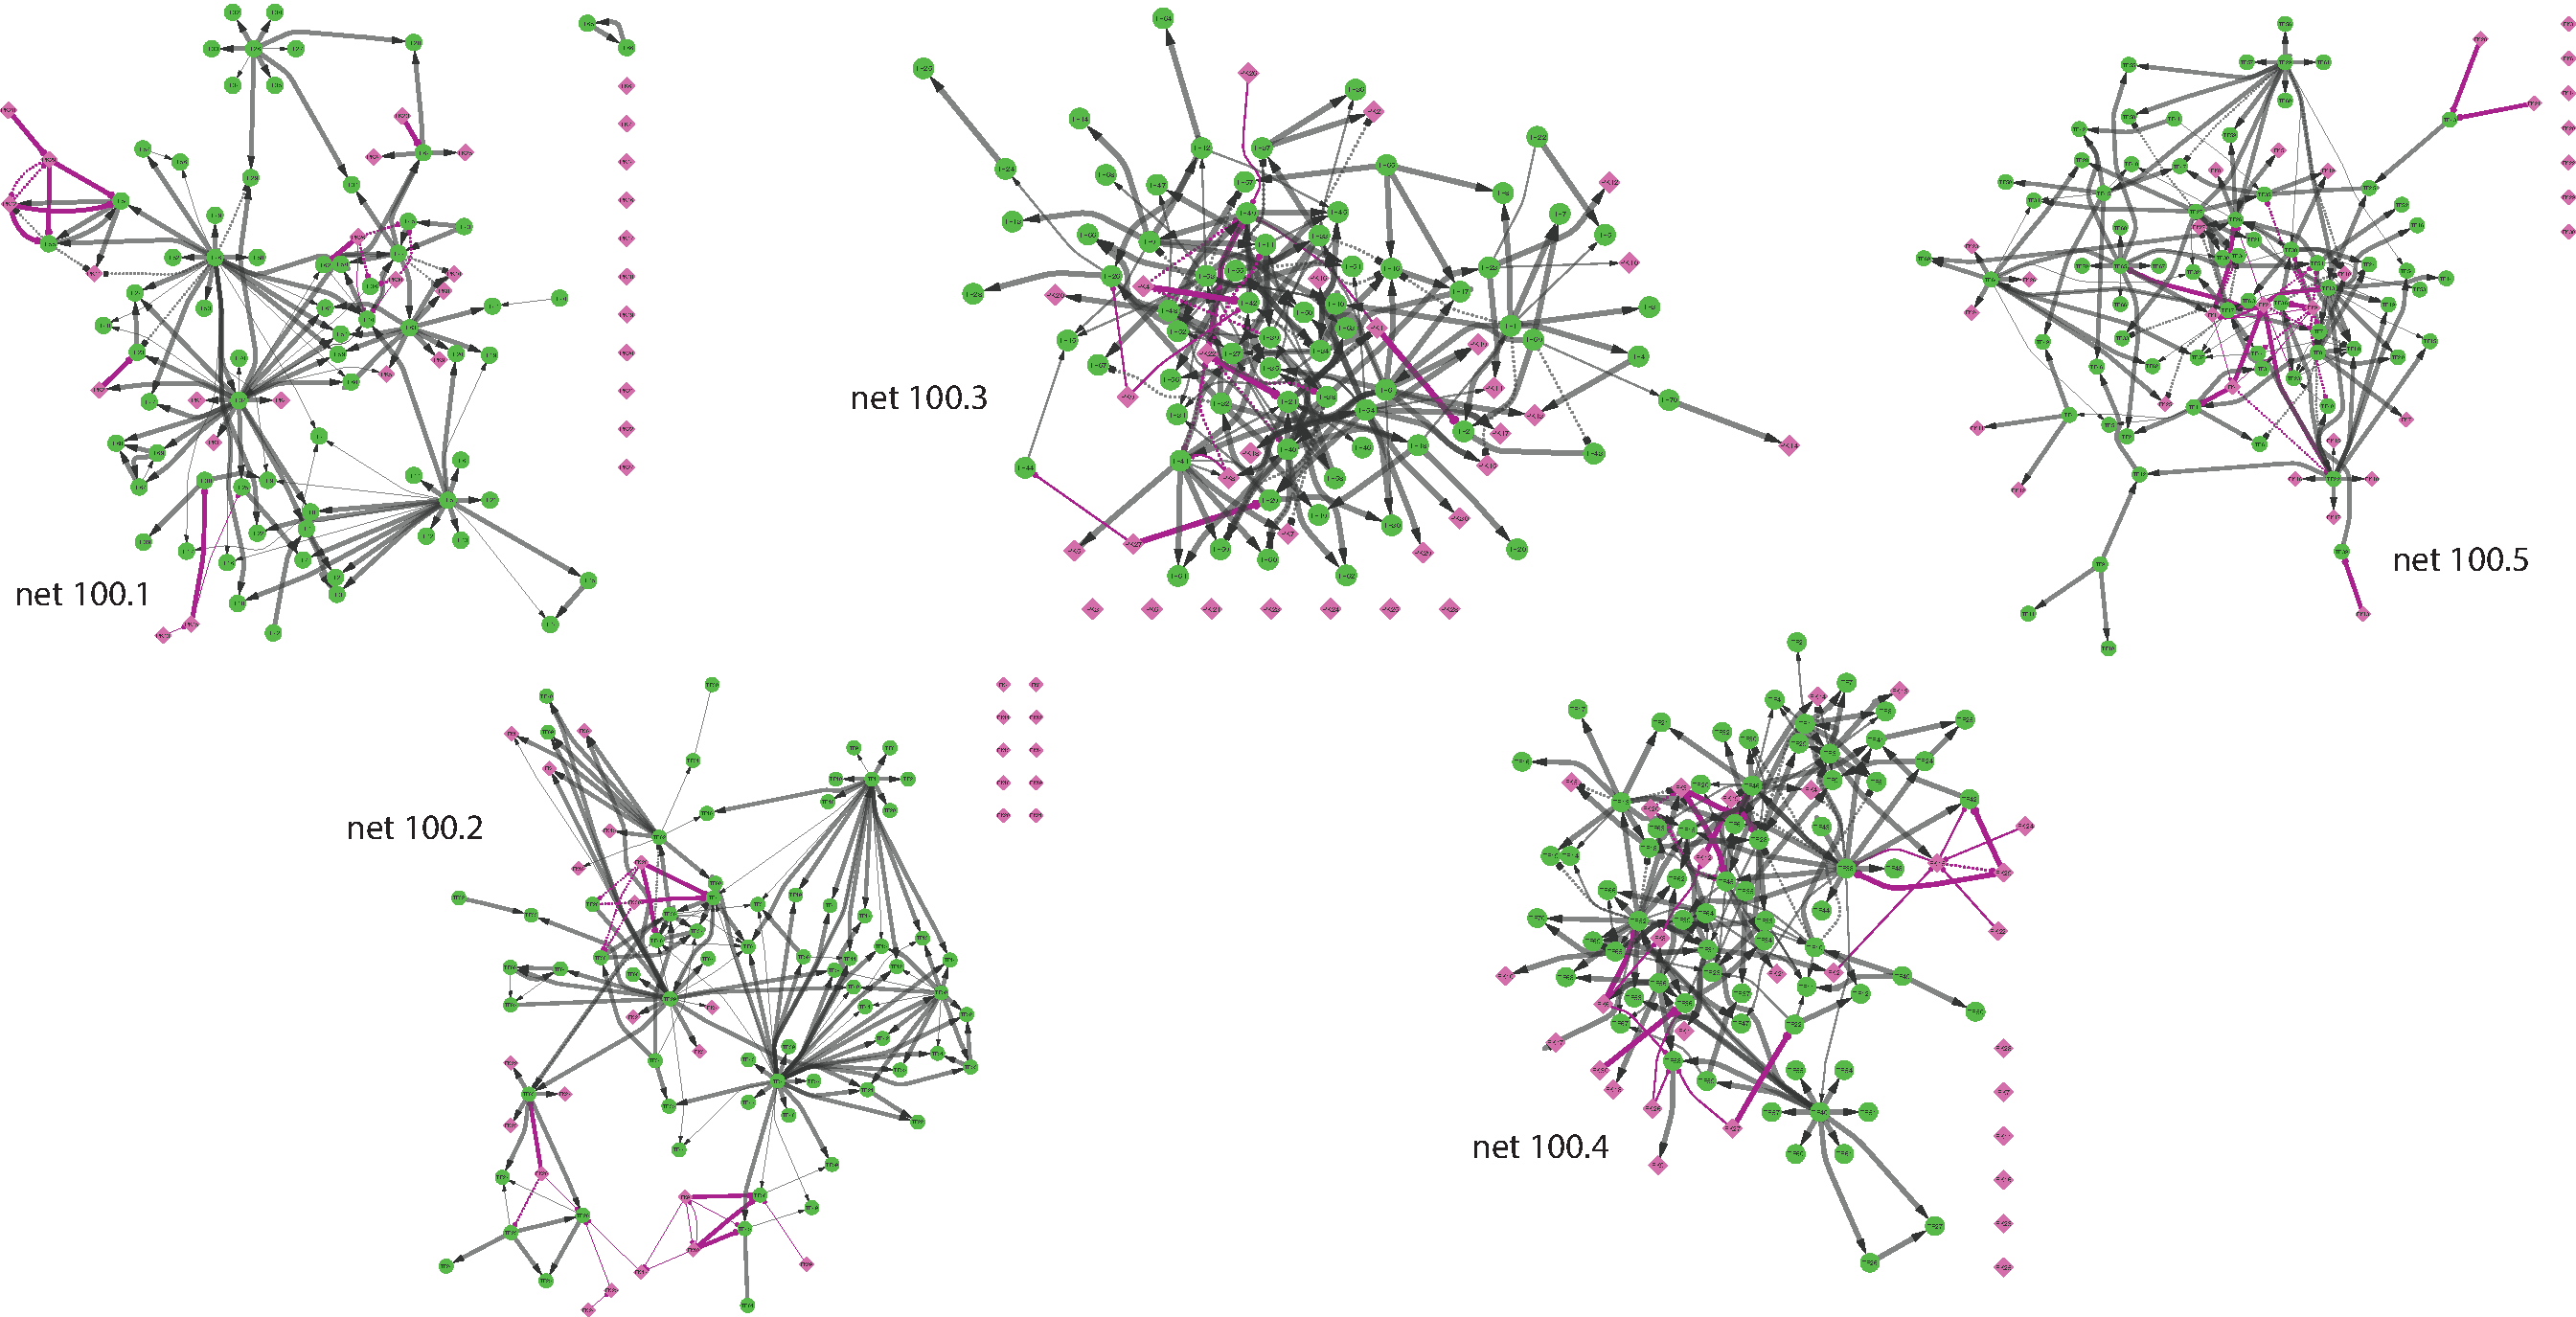
\includegraphics[width=.93\textwidth]{analysis/fig/dream100_infer_pres.pdf}
    \caption{\textbf{Inferred edges of 5 100-node networks.} Edge inferred from single $\boldsymbol{e}$-minimization when $w>0.01$. \textbf{Thick line} = TP, thin = FN, dotted = FP, none = TN. \textcolor{gray}{Dim line} = TF edge, \textcolor{pk!50!magenta}{magenta} = PK edge. }
    \label{fig:dream_100_infer}
\end{figure}
\end{frame}


% \begin{frame}{Protein kinase interaction inference on yeast data}
% \label{sec:yeast_results}
% \begin{columns}
% \newcommand\histwidth{0.36\textwidth}
% \begin{column}{0.5\textwidth}
% % The TF$\rightarrow$gene edges from the data are assumed to be the full set of transcription factors and the signs of their interactions are also enforced for edges where it is known in the Yeastract dataset, as described in~\autoref{sec:data_preprocess}. The inference is performed on edges with protein kinases as source node. For TFs, the model predicts edge strengths, and, in cases with unknown sign, it predicts the sign of interaction.


% \begin{figure}[ht]
% \centering
% \begin{subfigure}[b]{\histwidth}\centering\caption{}
% 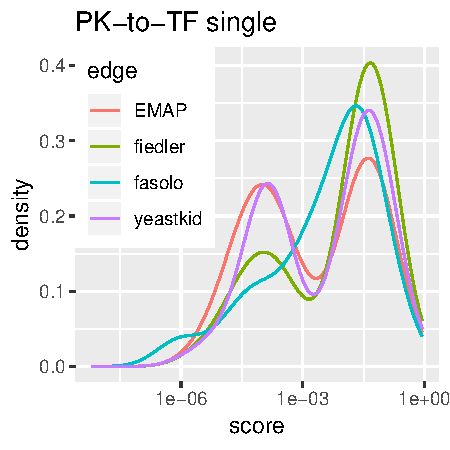
\includegraphics[width=\textwidth]{analysis/fig/hist_pk-tf_high_single.pdf}\label{fig:yeast_hist_single.a}
% \end{subfigure}
% \quad
% \begin{subfigure}[b]{\histwidth}\centering\caption{}
% 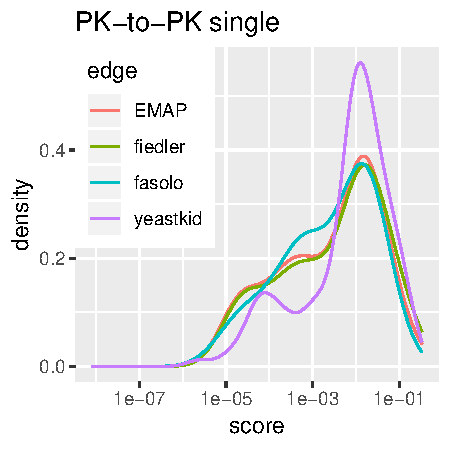
\includegraphics[width=\textwidth]{analysis/fig/hist_pk-pk_high_single.pdf}\label{fig:yeast_hist_single.b}
% \end{subfigure}
% % \vskip\baselineskip
% \begin{subfigure}[b]{\histwidth}\centering\caption{}
% 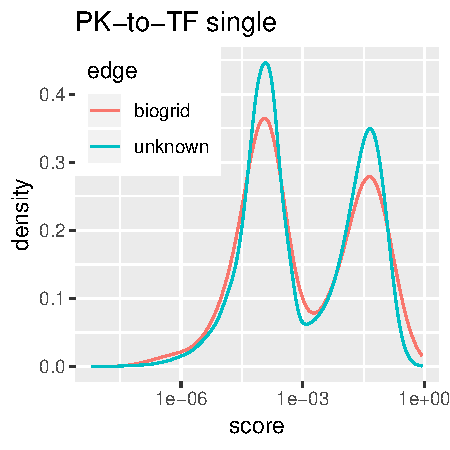
\includegraphics[width=\textwidth]{analysis/fig/hist_pk-tf_single.pdf}\label{fig:yeast_hist_single.c}
% \end{subfigure}
% \quad
% \begin{subfigure}[b]{\histwidth}\centering\caption{}
% 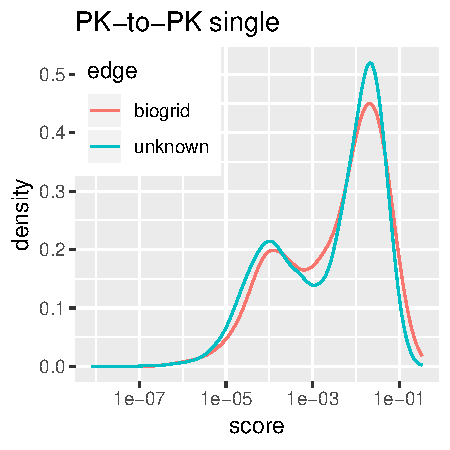
\includegraphics[width=\textwidth]{analysis/fig/hist_pk-pk_single.pdf}\label{fig:yeast_hist_single.d}
% \end{subfigure}
% \caption{\textbf{PK edge inference on yeast.} High quality edges~(a,b) and unknown/less likely edges~(c,d). }
% \label{fig:yeast_hist_single}
% \end{figure}

% % Edge inference was attempted on the RNA log fold-change data~(\autoref{sec:yeast_data}). Densities of scores for edges from different datasets can be seen in~\autoref{fig:yeast_hist_single} for a single attempt at minimizing~$\boldsymbol{e}$ where the score is the absolute weight value, and in~\autoref{fig:yeast_hist_avgstd} normalized scores where multiple individual attempts at minimizing~$\boldsymbol{e}$ were performed and normalized so that the scores are average weight values divided by the empirical standard deviation observed for each. The LLC method was used for comparison which can be found in~\autoref{fig:yeast_hist_llc} in the appendix, where it can be seen that there is no clear difference between datasets. Inference was also attempted by letting the score of an edge be the average weight from multiple individual minimization of~$\boldsymbol{e}$, with similar results to the normalized attempt~(\autoref{fig:yeast_hist_avg}). All density plots are split into subplots for datasets where we expect all edges should be true edges and the low confidence datasets biogrid and the category "unknown" which holds all entries of the adjacency matrix where an edge is possible, yet not found in any of the other datasets.

% \end{column}
% \begin{column}{0.5\textwidth}
% \begin{figure}[ht]
% \centering
% \begin{subfigure}[b]{\histwidth}\centering\caption{}
% 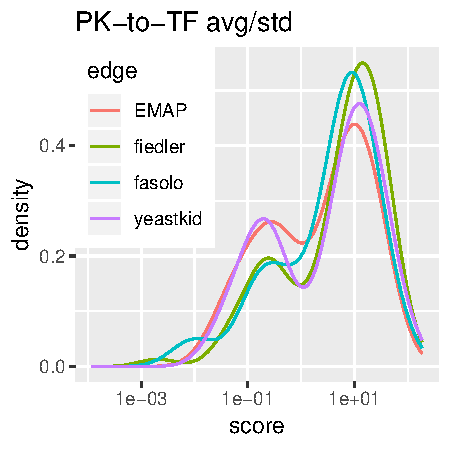
\includegraphics[width=\textwidth]{analysis/fig/hist_pk-tf_high_avgstd.pdf}
% \end{subfigure}
% \quad
% \begin{subfigure}[b]{\histwidth}\centering\caption{}
% \includegraphics[width=\textwidth]{analysis/fig/hist_pk-pk_high_avgstd.pdf}
% \end{subfigure}
% % \vskip\baselineskip
% \begin{subfigure}[b]{\histwidth}\centering\caption{}
% \includegraphics[width=\textwidth]{analysis/fig/hist_pk-tf_avgstd.pdf}
% \end{subfigure}
% \quad
% \begin{subfigure}[b]{\histwidth}\centering\caption{}
% \includegraphics[width=\textwidth]{analysis/fig/hist_pk-pk_avgstd.pdf}
% \end{subfigure}
% \caption{\textbf{Normalized PK edge inference on yeast.} High quality edges~(a,b) and unknown/less likely edges~(c,d). }
% \label{fig:yeast_hist_avgstd}
% \end{figure}
% \end{column}
% % We observe that two peaks appear in the density plots, at around score=\num{1e-4} and score=\num{3e-2} for~\autoref{fig:yeast_hist_single} as well as score=\num{1e-1} and score=\num{1e+1} for~\autoref{fig:yeast_hist_avgstd}. The peaks are visible for PK$\rightarrow$TF edges but PK$\rightarrow$PK edge inference is not clearly divided. The peaks can be useful for categorizing edges as present or absent, with the peak at lower score classifying absence of edges and the other indicating presence. We see that for datasets with edges assumed to be known, there are higher densities for peaks at higher scores~(\autoref{fig:yeast_hist_single.a}). This is especially seen for Fasolo~et~al. data but barely for EMAP data~\autoref{sec:fiedler_data}. The opposite is the case for datasets where the edge presence and absence are unknown~(\autoref{fig:yeast_hist_single.c}). Since the adjacency matrices should overall be sparse there would be many non-edges. 
% \end{columns}
% \end{frame}

\begin{frame}{Inference performance}
\begin{columns}
\begin{column}{0.2\textwidth}
Simulated data 
Yeast data
\begin{itemize}
    \item No negative examples
    \item Few datapoints
\end{itemize}
\end{column}

\begin{column}{0.8\textwidth}
\begin{figure}[ht]
    \centering
    \includegraphics[width=0.85\textwidth]{analysis/fig/Fig3.pdf}
    \caption{\textbf{Performance on simulated and yeast data.} \\  }
    \label{fig:minimum_performance}
\end{figure}
% Since the datasets for evaluation of performance only provides examples of presence of edges~(positive examples), we cannot directly evaluate balance between accuracy, specificity, etc. for the model. By using all possible edges not in a dataset of known edges we get a minimum performance where many of the datapoints used as negatives are in fact positives~(\autoref{fig:minimum_performance}). The Fiedler dataset with PK$\rightarrow$TF edges is included, since it was the single dataset with best performance. We see that PK$\rightarrow$PK edges from any dataset has no noticeably higher scoring than edges not in the dataset. PK$\rightarrow$TF edges from the datasets with known edges has a clear but small overrepresentation as larger scoring edges compared to other possible edges.
\end{column}
\end{columns}
\end{frame}




\section{Discussion}
\begin{frame}{Discussion}
\begin{columns}
\begin{column}{0.5\textwidth}
% A few points of interest are discussed here, in consideration of the validity of the analysis performed.
\begin{itemize}
    \item<1-| handout:1-> The data
% The RNA expression levels for a gene that is knocked out should generally be very low and lower than what is the case for wildtype measurements, where it is not knocked out. We observe that PK measurements for genes that were supposedly knocked out are generally quite small, usually observed at around 8 times smaller concentrations than in wildtype~(\autoref{fig:KO_RNA_hist}). TF knockouts, however, are not as low in expression when knocked out. 
% This has been discussed extensively by Luscombe~et~al.~\cite{Luscombe2010}. 
% For genes that are already transcribed at low levels this can be an artifact of microarray studies letting through a weak signal for a gene that is no longer transcribed. If expression was low enough for the wildtype the noise can make it difficult to see a difference between the experimental conditions. 
% Otherwise the observed expression can be due to multiple expression sites where others are making up for a knocked out site.
% So we expect noise in the data and cannot ignore log fold-change values for genes naturally expressed at low levels since this would require knowledge of the absolute sizes of the measured concentrations of RNA.
    \begin{itemize}
        \item Microarray artifact for low level expression
        \item Expression redundancy
        \item Discussed by Luscombe~et~al.~\cite{Luscombe2010}
    \end{itemize}
    \item<2-| handout:2-> Linear models
    \begin{itemize}
        \item Non-linear measurement relationship
        % The linearity in the model is between node values $\boldsymbol{x}$. As they describe log fold-change measurements~(\autoref{eq:second_equilibrium_def}) the effects from the underlying measurements are non-linear, which we can see from the linear relations~(ignoring $\boldsymbol{e}$):
        \item Justified by GNW extension
        % Wildtype and knockout measurements are simulated separately with the GeneNetWeaver kinase extension with a combination of linear and non-linear regulation mechanics, as well as both direct and indirect effects of proteins. In edge inference on data simulated with GNW extension we see a reasonable performance~(\autoref{fig:micro_average}) which is the justification for allowing the assumption of linear relationships among log fold-change node values. A biological cell is however not a perfectly mixed solution of interacting nodes. There are compartmentalization, dependency on time and cell cycle, as well as many other molecules not accounted for, which we might interpret are all important factors based on the results for experimental data.
        \item Non-linear convergence models
        % The applied equilibrium model~(\autoref{sec:equilibrium_model}) is linear in order to allow for the iterative calculations of node values through discrete time to reach equilibrium as an equation that can be formulated analytically~(for instance in~\autoref{eq:first_equilibrium_def}). Describing non-linear regulation would require a convergence model instead~(\autoref{sec:convergence_model}), where, starting at wildtype node values, the non-linear regulation system is used iteratively until convergence where the predicted values can be compared to measured equilibrium values in order to perform a gradient descent of model parameters. Using a convergence model increases computational cost significantly since a full convergence of a nonlinear system has to occur for every step of gradient descent.
    \end{itemize}
    \item<3| handout:3> Underdetermination
    \begin{itemize}
        \item Parameter count vs. data available
% Excessive parameter count was a concern since we are considering directed edges between all regulatory proteins. It was a consideration if there are too many model parameters to be determined from the available data.
        \item Top-down vs. bottom-up model design~\cite{Nielsen2017}
% A simpler model will have fewer parameters to determine and will be closer to be fully determined given the data than a more complicated model which might describe the dynamics of gene regulation more realistically. A model has to be designed with this balance between realism and parameter count in mind. 
% The ideal case is a model design on detailed gene regulation equations where parameters can cancel out due to the relative aspect of the measurements or if it can otherwise be justified to ignore them. The model applied here is instead designed top-down which is a far easier task, but it cannot be assumed to be accurate without the evidence from in-silico experiments.
    \end{itemize}
    \item<3| handout:3> Assumptions
    \begin{itemize}
        \item Equilibrium
        \item TF regulons
% We apply knowledge of edges in the graph believed to be present from experimental data by not allowing other edges to be nonzero, also referred to as masking the adjacency matrix. The entries not forced to be zero are also referred to as trainable parameters. It was applied for transcription factor to gene edges since there is a wealth of those interactions available. Forcing other possible edges to be nonzero leaves out the option of novel edge discovery but is a simple approach when there are many interactions known. It was also attempted to regulate the edges in a way that allows for TF edge discovery outside the given datasets, which can be done by masking the regularization, in order to have different regularization strengths for individual parameters to promote edges found in the datasets.

% Masking the adjacency matrix, however, does not force all edges in the dataset to be used. The method finds the optimal parameter values for each trainable parameter, and that value can be zero, in cases where that is optimal. For this reason the masking matrix should ideally be an overestimate of the true edges rather than an underestimate but if there are false edges in the dataset it will bias the method of inference to use them.
        \item RNA represent protein
% The Equilibrium model uses log fold-change protein values which are represented with the RNA log fold-change given in the data. The correlation between protein and RNA is sometimes as low as 0.6 so the RNA values might introduce some uncertainty to the model. The assumption that the protein values can be represented with RNA values is a natural result of assuming that the measurements are taken at an equilibrium if we apply the differential equations for translation~(\autoref{eq:prot_RNA}).
% So as we approach equilibrium we assume that our mRNA measurements adequately can describe a corresponding protein ratio or log fold-change.
% The issue is the assumption of a linear effect from RNA to protein in the model, so it is the hope that the nature of comparing the expression levels to wildtype will be better correlated than the absolute measurement values.
    \end{itemize}
\end{itemize}
\end{column}
\begin{column}{0.5\textwidth}
\alt<1| handout:1>{\begin{figure}[ht]
  \centering
  \includegraphics[width=\textwidth]{data/fig/knockout_RNA_hist.pdf}
  \caption{\textbf{KO RNA expression level histogram.} Subfig.~\ref{fig:KO_RNA_hist}. }
\end{figure}}
{\stepcounter{figure}}
\alt<2| handout:2>{
\begin{subequations}
\label{eq:discussion_linear}
\begin{align}
x_i &= \sum_j b_{ij} x_j
\\
\log \frac{x_i^{(ko)}}{x_i^{(wt)}} &=
\sum_j b_{ij} \log \frac{x_j^{(ko)}}{x_j^{(wt)}}
\\
\frac{x_i^{(ko)}}{x_i^{(wt)}} &=
\prod_j \left( \frac{x_j^{(ko)}}{x_j^{(wt)}} \right) ^{b_{ij}}
\end{align}
\end{subequations}}
{\stepcounter{equation}}
\alt<3| handout:3>{\begin{subequations}
\label{eq:prot_RNA}
\begin{align}
\dv{p_i}{t} &= m_i r_i - \lambda_i p_i
\\
\frac{p_i^{(ko)}}{p_i^{(wt)}} &= \frac{m_i r_i^{(ko)} - \dv{p_i^{(ko)}}{t}}{m_i r_i^{(wt)} - \dv{p_i^{(wt)}}{t}}
\end{align}
\end{subequations}
For $\dv{p_i^{(ko)}}{t} \rightarrow 0$ and $\dv{p_i^{(wt)}}{t} \rightarrow 0$ we then get
\begin{equation}
x_i =
\log \frac{p_i^{(ko)}}{p_i^{(wt)}} = \log
\frac{r_i^{(ko)}}{r_i^{(wt)}}
\end{equation}}
{\stepcounter{equation}}
\end{column}
\end{columns}
\end{frame}

\section{Conclusion}
\begin{frame}{Conclusion}
\begin{itemize}
    \item Graph learning beyond DAGs, TFs, and small graphs
% Many methods and models have been proposed and examined for graph inference, but each have details separating them from the work discussed here. Many either rely on DAGs, or model direct interactions, which often completely ignores protein kinases and instead only focuses on transcription factors. The justification is often that transcription factors are complicated enough on their own, which can be interpreted from the results in section~\autoref{sec:yeast_results}. It is found that the method clearly outperform LLC on the indirect edges from PKs. It is found that the indirect evidence of protein interaction gathered from knockout studies are not convincingly useful by itself for inference, but does seem to add useful information.

% We demonstrate, that it is possible to simulate non-linear and complex gene regulation involving protein kinases, and infer the underlying interactions, in spite of the much larger space of parameters defining the simulations~(\autoref{sec:dream_results}). It is also demonstrated that performance can be improved significantly with a novel loss function~(\autoref{sec:cascade_loss}).
    \item Future work
    \begin{itemize}
        \item PK$\rightarrow$TF vs PK$\rightarrow$PK preference
        \begin{itemize}
            \item Outgoing edges usually sum to <1 for mediating PK
% When an effect from a protein kinase knockout is observed across a node value, the equilibrium method can choose to infer an edge to the most obvious transcription factor or infer an edge to another protein kinase that are found to regulate the same transcription factors~(\autoref{sec:toy}).
% If we use L1-regularization for PK edges the latter is only favored in the case where the weights from the other PK sum to more than 1.
% Testing the performance improvements possible with the alternative loss function described in~\autoref{sec:cascade_loss} would be interesting for simulated data on larger networks. It could be a great way to improve performance on simulated data, however, it is unclear how much this would help for experimental data.
        \end{itemize}
    \item Exploiting other data types
% As discussed in~\autoref{sec:evolution} there are potential in interspecies data, which can be exploited in order to take advantage of data from similar species, instead of studying a strain in isolation. This can especially be useful if one were to study an organism which is not a major model organism as has been done here. It can be implemented into the current model by defining a new loss function inspired by the one applied by Kashima~et~al.~\cite{Kashima2009}. Their method was however inferring undirected edges for enzyme interactions, which can be a problem to consider if we are interested in directed edges.
        \begin{itemize}
            \item Evolutionary cost
            \item Interspecies protein similarity 
            % ($\text{W}^{(k,l)}, k \ne l$)
            \item Intraspecies gene expression similarity 
            % ($\text{W}^{(k,l)}, k = l$)
            \item Multiple observations of same KO
        \end{itemize}
    \item Further extension to GeneNetWeaver
% It could be interesting to increase model realism, for instance by considering cell compartmentalization, cell cycle, time-dependence of processes, allowing proteins more than two phosphorylation states etc.
% Currently, the GeneNetWeaver kinase extension was written to use kinases as the signal transducing proteins and phosphatases collectively included in the model by the constant decay of phosphates on phosphorylated proteins~(\autoref{sec:gnw_extension}). Although, allowing negative protein kinase edges, corresponding to targeted dephosphorylation, was tested to work without issue~(\autoref{fig:micro_average.d}).
% Transcription factors can both have an active form as phosphorylated and as unphosphorylated. Allowing the unphosphorylated transcription factor to serve an active regulation role could be a further extension to increase realism of simulation.
    \begin{itemize}
        \item Phosphorylation $\ne$ activity
        \item Nondimensionalization
    \end{itemize}
\end{itemize}
\end{itemize}
\end{frame}

\begin{frame}{Nondimensionalized kinase regulation model}
\begin{columns}
\begin{column}{0.7\textwidth}
Kinase cascade, each protein with single input
\begin{subequations}
\begin{align}
\dv{\phi_i}{t} &=
    w_i \phi_{i-1} \left(p_i - \phi_i\right) - \lambda_i^{(\text{Phos})} \phi_i    
\\
    &=
    \frac{\hat{w}_i}{p_{i-1}^{(\text{max})}} \hat{\phi}_{i-1} p_{i-1}^{(\text{max})} \left(\hat{p}_i p_i^{(\text{max})} - \hat{\phi}_i p_i^{(\text{max})} \right) - \lambda_i^{(\text{Phos})} \hat{\phi}_i p_i^{(\text{max})}
\\
\phi_i &= \hat{\phi}_i p_i^{(\text{max})} \implies
\\
\dv{\hat{\phi}_i}{t} &=
    \hat{w}_i \hat{\phi}_i \left(\hat{p}_i - \hat{\phi}_i\right) - \lambda_i^{(\text{Phos})} \hat{\phi}_i
\end{align}
\end{subequations}
Generalized, any protein can affect any protein
\begin{subequations}
\begin{align}
\dv{\hat{\phi}_i}{t} &=
    \left( \sum_j \hat{w}_{ij} \hat{\phi}_j \right) \left(\hat{p}_i - \hat{\phi}_i\right) - \lambda_i^{(\text{Phos})} \hat{\phi}_i
\\
\dv{\hat{\boldsymbol{\phi}}}{t} &= 
    \left(\hat{W} \hat{\boldsymbol{\phi}}\right) \left(\hat{\boldsymbol{p}} - \hat{\boldsymbol{\phi}}\right) - \Lambda_\text{Phos} \hat{\boldsymbol{\phi}}
\end{align}
\end{subequations}
Before: $\dv{\boldsymbol{\phi}}{t} = (W \boldsymbol{\phi}) \left(1 - \frac{\boldsymbol{\phi}}{\boldsymbol{p}}\right) - \Lambda_\text{Phos} \boldsymbol{\phi}$
\end{column}

\begin{column}{0.3\textwidth}
\begin{figure}
\begin{minipage}[c]{0.617\textwidth}
\includegraphics[width=\textwidth]{theory/fig/kinase_cascade.pdf}
\end{minipage}
\end{figure}
\end{column}
\end{columns}
\end{frame}



\section*{Questions}


\appendix
\begin{frame}[allowframebreaks]{References}
\printbibliography[heading=none]
\end{frame}
\end{document}